% -----------------------------------------------------------------
%        File: thesis.tex
% Description: Thesis
%      Author: Andrew Parlane
% -----------------------------------------------------------------

% This file is part of https://github.com/andrewparlane/fiuba_thesis
% Copyright (c) 2022 Andrew Parlane.
%
% This is free software: you can redistribute it and/or modify it under
% the terms of the GNU General Public License as published by the Free
% Software Foundation, version 3.
%
% This program is distributed in the hope that it will be useful, but
% WITHOUT ANY WARRANTY; without even the implied warranty of
% MERCHANTABILITY or FITNESS FOR A PARTICULAR PURPOSE. See the GNU
% General Public License for more details.
%
% You should have received a copy of the GNU General Public License
% along with this code. If not, see <http://www.gnu.org/licenses/>.

% Note: This thesis should be compiled from the version in the repository
%       via the Makefile and not by overleaf. Overleaf should work
%       but the formatting has been checked with the version compiled from the Makefile.

\documentclass[a4paper, twoside, 11pt]{report}

% =============================================
% Includes
% =============================================

% packages
% -----------------------------------------------------------------
%        File: packages.tex
% Description: Various packages
%      Author: Andrew Parlane
% -----------------------------------------------------------------

% This file is part of https://github.com/andrewparlane/fiuba_thesis
% Copyright (c) 2022 Andrew Parlane.
%
% This is free software: you can redistribute it and/or modify it under
% the terms of the GNU General Public License as published by the Free
% Software Foundation, version 3.
%
% This program is distributed in the hope that it will be useful, but
% WITHOUT ANY WARRANTY; without even the implied warranty of
% MERCHANTABILITY or FITNESS FOR A PARTICULAR PURPOSE. See the GNU
% General Public License for more details.
%
% You should have received a copy of the GNU General Public License
% along with this code. If not, see <http://www.gnu.org/licenses/>.

% Maths stuff (\begin{align*} for one)
\usepackage{amsmath}

% Spanish Localisation
\usepackage[spanish]{babel}

% UTF8 encoding allows for accents. Must come before biblatex
\usepackage[utf8]{inputenc}

% Bibliography
\usepackage[backend=biber, style=numeric]{biblatex}

% For \captionsetup
\usepackage{caption}

% Required by biblatex and must come after inputenc
\usepackage{csquotes}

% dirtree (for outputting the dir tree of the repos)
\usepackage{dirtree}

% Better lists, allows setting \parsep
\usepackage{enumitem}

% A4 + default margins
\usepackage[a4paper]{geometry}

% Images
\usepackage{graphicx}

% For embedding code
\usepackage{listings}

% Multirow
\usepackage{multirow}

% for \nicefrac
\usepackage{nicefrac}

% For \onehalfspacing
\usepackage{setspace}

% For \FloatBarrier
\usepackage{placeins}

% SI Units
\usepackage{siunitx}

% Allows for setting space between sections
\usepackage[compact]{titlesec}

% Links (must be loaded after titlesec)
\usepackage{hyperref}

% Fix links to images so they actually show the image
\usepackage[all]{hypcap}

% TabularY (for autosizing columns (L) in the port list tabels)
\usepackage{tabulary}

% Change spacing around ToC
\usepackage{tocloft}

% Colours for table row zebras
\usepackage[table]{xcolor}


% settings
% -----------------------------------------------------------------
%        File: settings.tex
% Description: Various configuration settings
%      Author: Andrew Parlane
% -----------------------------------------------------------------

% This file is part of https://github.com/andrewparlane/fiuba_thesis
% Copyright (c) 2022 Andrew Parlane.
%
% This is free software: you can redistribute it and/or modify it under
% the terms of the GNU General Public License as published by the Free
% Software Foundation, version 3.
%
% This program is distributed in the hope that it will be useful, but
% WITHOUT ANY WARRANTY; without even the implied warranty of
% MERCHANTABILITY or FITNESS FOR A PARTICULAR PURPOSE. See the GNU
% General Public License for more details.
%
% You should have received a copy of the GNU General Public License
% along with this code. If not, see <http://www.gnu.org/licenses/>.


% Don't indent paragraphs
\setlength{\parindent}{0cm}

% Space between paragraphs
\parskip 1.5ex

% Line spacing: 1.5
\onehalfspacing

% Reduce space between items in \begin{description}, \begin{itemize} and \begin{enumerate}
\setlist[description]{noitemsep, nolistsep, topsep=0pt}
\setlist[itemize]{noitemsep, nolistsep, topsep=0pt}
\setlist[enumerate]{noitemsep, nolistsep, topsep=0pt}

% Change Table of Contents name from "Índice General" to "Índice"
\addto\captionsspanish{
  \renewcommand{\contentsname}
    {Índice}
}

% \Chapter format - Huge, bold, no numbering
\titleformat{\chapter}{\normalfont\Huge\bfseries}{}{0pt}{}

% Reduce space before and after the \chapter title
\titlespacing{\chapter}{0pt}{-1em}{1em}

% \Section format - huge, bold
\titleformat{\section}{\normalfont\huge\bfseries}{\thesection}{0pt}{}

% \Subsection format - LARGE, bold
\titleformat{\subsection}{\normalfont\LARGE\bfseries}{\thesection}{0pt}{}

% \subsubsection format - Large
\titleformat{\subsubsection}{\normalfont\Large}{\thesection}{0pt}{}

% Don't number sections
\setcounter{secnumdepth}{0}

% Sets links to blue
\hypersetup{
    colorlinks,
    citecolor=blue,
    filecolor=blue,
    linkcolor=blue,
    urlcolor=blue
}

% ToC depth to \subsubsection
\setcounter{tocdepth}{3}

% Remove spacing at top of page before and after the Índice title
\setlength{\cftbeforetoctitleskip}{0pt}
\setlength{\cftaftertoctitleskip}{0pt}

% Don't hyphonate over pages
\brokenpenalty10000\relax

% Captions should "hang" aka align with the start, and not with the label
\captionsetup{format=hang}

% Create a new command for referencing figures with "Figura ?.?" as the link. Same for tables and sections
% Call with:
%  \figref{fig:figure-label} 
%  \tabref{tab:table-label}
%  \secref{sec:section-label}{Section Name}
\newcommand*{\figref}[1]{\hyperref[#1]{Figura~\ref*{#1}}}
\newcommand*{\tabref}[1]{\hyperref[#1]{Cuadro~\ref*{#1}}}
\newcommand*{\secref}[2]{\hyperref[#1]{Sección #2}}

% Zebra pattern in tables
\newcommand*{\tablezebra}{\rowcolors{2}{white}{lightgray!35}}

% Let's us restart the row num to reset the zebra pattern using \setcounter{rownum}{0}
\makeatletter
\@ifundefined{c@rownum}{\let\c@rownum\rownum}{}
\makeatother


% Bibliography
\addbibresource{bibliography.bib}

% =============================================
% Document
% =============================================

\begin{document}

% ---------------------------------------------
% Title Page
% ---------------------------------------------
\begin{titlepage}

\capstartfalse
\begin{figure}
\centering
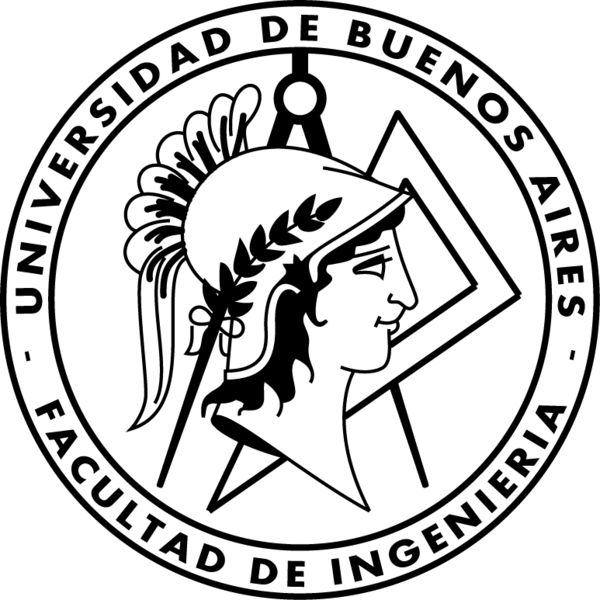
\includegraphics[scale=1.7]{./img/logo-facu.png}
\end{figure}
\capstarttrue

\begin{center}
    \Large{Universidad de Buenos Aires} \\
    \Large{Facultad de Ingeniería} \\
    \Large{Tesis de Maestría en Ciencias de la Ingeniería} \\
    \vspace{5mm}
    \huge{\bf Desarrollo de Circuitos Integrados CMOS para Aplicaciones de RFID} \\
    \vspace{8mm}
    \huge{\bf Andrew Parlane} \\
    \vspace{8mm}
    \huge{\bf Junio de 2022}
\end{center}

\vspace*{\fill}

\begin{description}
    \item[\large{Director:}] \hspace{21pt} \large{Dr. Ing. Mariano Garcia-Inza}
    \item[\large{Codirectores:}] \large{Ing. Federico G. Zacchigna, Ing. Octavio Alpago}
\end{description}
\end{titlepage}

% ---------------------------------------------
% Resumen
% ---------------------------------------------

\FloatBarrier
%\chapter* so it doesn't get added to the ToC
\chapter*{Resumen}
Este trabajo presenta el diseño de circuitos integrados digitales para la implementación de un TAG RFID en un chip CMOS. Los requerimientos de los circuitos son definidos por un proyecto de investigación marco cuyo objetivo general es el desarrollo de sensores inalámbricos de radiación ionizante para dosimetría médica. Esto requiere la integración de diferentes subsistemas en un ASIC a fabricar en tecnología CMOS.

Los circuitos presentados en esta tesis consisten en un bloque digital de control, que puede recibir y responder a las tramas definidas en la norma ISO/IEC 14443A, y mediante un protocolo propietario encima de la norma, controlar otros subcircuitos del chip necesarios para la adquisición de la señal dosimétrica y su posterior transmisión inalámbrica. La implementación de la norma es presentada en un núcleo IP genérico. Por lo tanto es apto para uso en otros proyectos y con cualquier lector comercial que trabaje bajo norma. El protocolo propietario consiste en cinco mensajes que permiten el muestreo de hasta quince TAGs de forma sincronizada. El muestreo simultáneo de múltiples TAGs sensores utilizando RFID es una estrategia novedosa desarrollada en esta tesis, el cual representa un potencial avance en el desarrollo de métodos de control dosimétrico en aplicaciones médicas.

El trabajo realizado incluye el diseño de los bloques digitales utilizando HDL SystemVerilog y su verificación funcional. Luego, se utiliza el kit de diseño del proceso (PDK, por sus siglas en Inglés) XH018 (nodo tecnológico de \SI{180}{\nano\meter}) de la foundry XFAB para realizar la síntesis, el place and route y la generación de las máscaras de fabricación (layout).

Las pruebas de verificación llevadas a cabo dan alta confianza en el diseño. Las mismas incluyen: 60 horas de simulaciones del RTL ejecutando 187 aserciones de SystemVerilog casi cien millones de veces y generando informes de cobertura de código, la verificación formal de equivalencia entre lógica RTL y los netlists post síntesis y post implementación, Design Rules Check (DRC), y Layout Vs Schematic (LVS); todas esas pruebas tienen resultados favorables.

El layout final no tiene violaciones de timing, el slack de Setup menor es \SI{1,59}{\nano\second} y de Hold es \SI{0,02}{\nano\second}, el área utilizada es \SI{0,087}{\milli\meter\squared} (\SI{295,68}{\micro\meter} por \SI{294,00}{\micro\meter}), y la estimación de consumo de potencia promedio es \SI{256}{\micro\watt}.

% ---------------------------------------------
% Aclaraciones
% ---------------------------------------------

\FloatBarrier
%\chapter* so it's not in the ToC
\chapter*{Aclaraciones}

Aclaraciones
Por cuestiones de claridad en esta tesis cuándo se dice que una señal está en ‘1’ o ‘0’ significa que la señal tiene un valor lógico igual a '1' o ‘0’ respectivamente.

El código RTL, los bancos de pruebas y los scripts de síntesis y place \& route están publicados de forma abierta en GitHub bajo la licencia GNU v3.0, de manera que cualquier parte de este trabajo pueda ser utilizada en otros proyectos académicos o comerciales. Para facilitar la adopción y modificación de este trabajo por la comunidad internacional, el código y los scripts están escritos con nombres y comentarios en Inglés. El enlace al repositorio y detalles de su estructura son dados en el \appref{appendix:code_repo}.

Para facilitar la lectura de esta tesis las señales, variables y parámetros están escritos en \textit{cursiva},  los módulos, clases y funciones están escritos en \textbf{negrita}. Además se utilizan paréntesis para nombrar a las funciones, aunque sin sus argumentos, por ejemplo: \textbf{compare()}. Finalmente los nombres de las tramas definidas en los protocolos están escritos en MAYÚSCULAS.

% ---------------------------------------------
% TOC
% ---------------------------------------------
\newpage
\tableofcontents

% ---------------------------------------------
% Introducción
% ---------------------------------------------

\FloatBarrier
\chapter{Introducción}

% Motivación y Contexto de Trabajo
% --------------------------------
\FloatBarrier
\section{Motivación y Contexto de Trabajo}

La radioterapia es un tratamiento médico que consiste en utilizar radiación ionizante para eliminar células cancerígenas que forman tumores. Sin embargo, la radiación puede presentar riesgos a tejido sano, especialmente si la dosis aplicada es mayor a la necesaria o mal localizada. Hay varios incidentes registrados donde algunas personas recibieron una sobredosis durante radioterapia, y en algunos casos dosis letales~\cite{accidentaly_exposures}. Por otro lado, una dosis localizada pero demasiado pequeña reduciría la efectividad del tratamiento. Por esas razones es muy importante adoptar consideraciones de QA (Quality Assurance), la cual puede definirse como:

\begin{displaycquote}[traducido de][]{qa_in_radiotherapy}
Los procedimientos que aseguren el cumplimiento de las prescripciones médicas con respeto a la dosis entregada al volumen deseado, junto con una dosis mínima a tejido sano, exposición mínima al personal, y el monitoreo adecuado del paciente para determinar el resultado del tratamiento.
\end{displaycquote}

Una técnica importante en QA es dosimetría in-vivo (IVD), que es la práctica de medir la dosis recibida durante el tratamiento. El uso de IVD es recomendado en radioterapia~\cite{AAPM-1994}\cite{ICRP-2000} y su aplicación requiere un error de medición menor al 3\% a lo largo del tratamiento. Existen varios tipos de sensores de radiación que pueden ser utilizados para IVD en radioterapia. Entre ellos se encuentran los sensores MOSFET, los cuales tienen varias ventajas, como por ejemplo que pueden ser leídos tanto en tiempo real como posteriormente, son pequeños y robustos, pero también tienen algunas limitaciones~\cite{electronic_dosimetry}. Los investigadores del Laboratorio de Física de Dispositivos - Microelectrónica de la Facultad de Ingeniería de la Universidad de Buenos Aires han trabajando durante los últimos años en mejorar el desempeño de sensores MOSFET de radiación para uso en IVD~\cite{mosfet_mismatch_amplification}\cite{6MV_LINAC}. Otra ventaja de los sensores MOSFETs es que pueden ser integrados en un mismo chip con circuitos adicionales que permitan su lectura, digitalización y posterior transmisión de los resultados en tiempo real. Esto representa una importante ventaja frente al método usual de lectura post irradiación, ya que el seguimiento en tiempo real permitiría ajustar la dosis durante la ejecución del tratamiento.

Un sensor pequeño construido con una cantidad mínima de componentes permitiría obtener arreglos de sensores con excelente resolución espacial y así realizar un mapeo dosimétrico de una zona de interés. A la hora de implementar esta solución, los TAGs RFID (Radio Frequency Identification) pasivos son una excelente opción, ya que sólo requieren del circuito integrado y una antena externa. La alimentación y la comunicación pueden realizarse a través del campo electromagnético generado por el dispositivo de lectura. Un sistema de estas características, además de ser más simple, sería más cómodo para el paciente y más práctico para su uso en el campo médico.

En su tesis de 2018~\cite{Arana_thesis}, Arana analizó la relación entre la frecuencia de operación de un TAG RFID y su distancia máxima de la lectura considerando los límites de exposición de humanos a campos electromagnéticos definidos en IEEE C95.1. Los resultados muestran que una frecuencia en el orden de 10 MHz daría el mejor rango de operación mientras manteniendo el campo electromagnético dentro de límites seguros. Esta frecuencia se encuentra cercana a los 13.56 MHz de RFID HF (High Frequency). Arana muestra en su tesis el diseño de la antena y de circuitos integrados analógicos para un TAG ISO/IEC 14443 tipo A que puede funcionar a una distancia de 30 cm de la lectura. También en una publicación de 2014~\cite{fabricio_eamta}, Alcalde et al. presentan el diseño y fabricación de un TAG RFID que implementa parte de la norma ISO/IEC 14443 tipo A. El funcionamiento es verificado a través de mediciones experimentales del sistema en loopback.

Un atributo del protocolo ISO/IEC 14443A es que permite hasta 15 TAGs activos al mismo tiempo. Esto da la posibilidad de obtener muestras de los sensores de forma sincronizada, con la ventaja de medir en múltiples lugares del cuerpo del paciente. Esto contribuye a mejorar la verificación de la ejecución del tratamiento planificado y por lo tanto se alinea con los criterios de QA.

En un artículo publicado en 2016~\cite{monolithic_180nm}, Villani et al. se desarrolló un sensor de radiación inalámbrico para IVD en radioterapia. El sensor emite una señal RF con frecuencia que depende de la dosis de radiación recibida. La ventaja de este enfoque es la simplicidad del diseño, el circuito integrado no necesita un bloque digital complejo para soportar el protocolo. Las desventajas son: solo es posible usar solo un sensor a la vez, requiere una fuente de alimentación externa (batería), no permite configurar el sensor inalámbricamente, y por no haber sido diseñado dentro de una norma, no es compatible con otros equipos requiriendo de un lector diseñado ad hoc para la aplicación.

Los circuitos diseñados en esta tesis permitirán implementar una red de sensores inalámbricos cuya finalidad es medir dosis de radiación en un tratamiento de radioterapia en diferentes lugares de interés. La adquisición en múltiples puntos tiene como objetivo mejorar el control de la irradiación para ajustar con mayor precisión la dosis entregada por el acelerador a la planificación previa. Típicamente, la dosis entregada por los LINAC es pulsada por lo cual, para que la medición en tiempo real sea útil, se requiere sincronizar el muestreo de los sensores.

% ISO/IEC 14443A
% --------------------------------
\FloatBarrier
\section{ISO/IEC 14443A}

La norma ISO/IEC 14443 fue desarrollada por la Organización Internacional de Normalización (ISO) y la Comisión Electrotécnica Internacional (IEC), específicamente por el grupo de tareas 2 del grupo de trabajo 8 de la subcomisión del comité técnico mixto 1. Fue publicado primero en 2001 con dos interfaces distintas: tipos A y B. Tipo A fue desarrollado en colaboración con Mikron (adquirida desde entonces por Phillips), basado en su tecnología Mifare. Esta interfaz fue diseñada como una tarjeta para almacenar datos únicamente. Tipo B fue desarrollado en colaboración con varios operadores de sistemas de transporte públicos de Europa e Innovatron. Principalmente diseñado para pagos de tarifas pero también puede funcionar como billetera electrónica y verificación de identidad. Esta interfaz fue diseñada como una tarjeta que al tener un microprocesador, además de almacenar datos, cuenta con capacidad de procesamiento. Al principio estas dos interfaces fueron complementarias, pero luego de los años sus aplicaciones se ampliaron y diversificaron~\cite{14443_a_vs_b}.

La norma viene en cuatro partes:

\begin{itemize}
    \item ISO/IEC 14443-1: Características Físicas.
    \item ISO/IEC 14443-2: Radiofrecuencia Potencia y Señal Interfaz.
    \item ISO/IEC 14443-3: Inicialización y Anticolisión.
    \item ISO/IEC 14443-4: Protocolo de Transmisión.
\end{itemize}

La parte 1 define atributos físicas de la PICC (Proximity Card, la tarjeta o TAG) como las dimensiones y el rango de operación a temperatura ambiente. La parte 2 define la interfaz inalámbrica de la transmisión de potencia y comunicaciones bidireccionales entre un PCD (Proximity Coupling Device, el lector) y la PICC. La parte 3 define el formato de los bytes, la estructura de las tramas y los mensajes necesarios para el descubrimiento y activación de todas las PICCs presentes en el campo del PCD. Finalmente, la parte 4 define un protocolo de bloques para la configuración de la PICC y la transmisión de mensajes de nivel aplicación.

Un sistema tiene un PCD que es el maestro y una o más PICCs que son las esclavas. Una PICC solo responde a solicitudes, no inicia comunicaciones. Durante el proceso de inicialización múltiples PICCs pueden responder a la misma solicitud, así que las colisiones son posibles y esperadas. Después del proceso de inicialización, en un sistema correctamente configurado, solo una PICC responde a cada solicitud.

\FloatBarrier
\subsection{ISO/IEC 14443-1: \large{Características Físicas}}

Esta parte de la norma define las condiciones de operación en cuáles la PICC debe poder funcionar correctamente. Estos requisitos son: la exposición máxima a rayos X, el límite dinámico de flexión y de torsión, la exposición a campos magnéticos y eléctricos alternos, la exposición a electricidad estática, y la temperatura ambiente\cite{iso14443-1}.

\FloatBarrier
\subsection{ISO/IEC 14443-2: \large{Radiofrecuencia Potencia y Señal Interfaz}}
\label{sec:introduction_iso14443-2}

El PCD emite un campo electromagnético con frecuencia $f_c = \SI{13.56}{\mega\hertz} \pm \SI{7}{\kilo\hertz}$. Las PICCs dentro de este campo se acoplan inductivamente al campo para la transferencia de potencia. El campo es modulado para la comunicación entre los dispositivos. El PCD usa modulación de amplitud para enviar información a las PICCs, y las PICC envían sus respuestas con modulación de carga mediante un subcarrier. La norma define varias tasas de bits, pero las comunicaciones siempre comienzan con tasa de bits $\nicefrac{f_c}{128} \approx \SI{106}{Kbps}$ en las dos direcciones. La codificación de los bits y los parámetros de modulación dependen de: la dirección de la comunicación, si las PICCs son tipo A o B, y la tasa de bits. La \figref{fig:mod-encode} muestra una representación de las dos direcciones de comunicación para PICCs de tipo A y de tipo B.

\begin{figure}[htb]
\centering
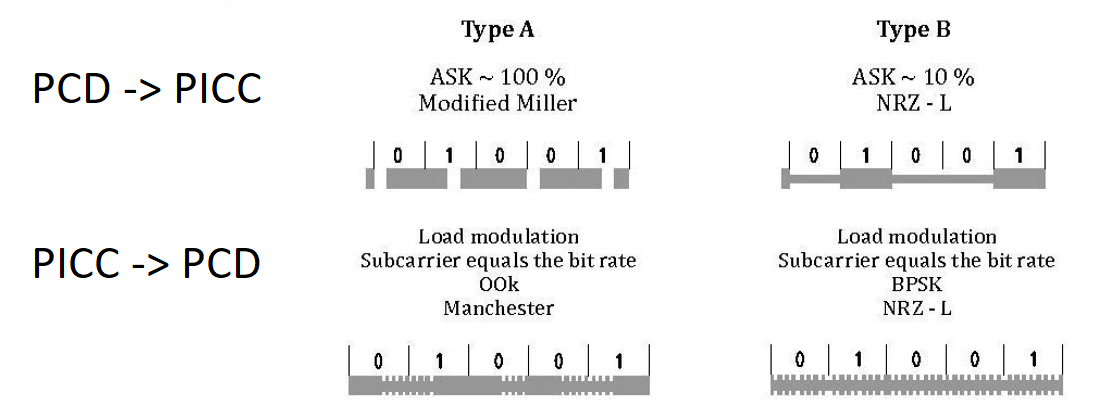
\includegraphics[scale=0.47]{./img/modulation_and_bit_encoding}
\caption{Comunicaciones con una tasa de bits de $\nicefrac{f_c}{128}$~\cite[Adaptado de][]{iso14443-2}}
\label{fig:mod-encode}
\end{figure}

Para PICCs de tipo A la modulación por comunicaciones desde el PCD hasta la PICC es ASK (Amplitude Shift Keying). Cuándo la amplitud de la portadora baja al 5\% del campo original, la norma define esto como una pausa. Un esquema de la misma se muestra en la \figref{fig:pause}, con valores que se definen en el \tabref{tab:pause_values}. Debido a que una PICC pasiva recibe su potencia inalámbricamente desde el campo electromagnético, es responsabilidad de la PICC mantener los rails de alimentación internos a tensiones adecuadas durante las pausas para que el sistema no cambie de estado. La codificación de los bits es Modified Miller. Cada trama comienza con un SOC (Start of Communication), tiene un número de bits de datos y termina con un EOC (End Of Communications). SOC, EOC y los valores lógicos son enviados mediante secuencias. Cada secuencia tiene el largo de una duración de bit, lo que es 128 ciclos de la portadora. La presencia y la ubicación de una pausa dentro de una duración de bit define el tipo de la secuencia, como es mostrado en la \figref{fig:sequences}. Una pausa que ocurre al principio de la duración de bit es una secuencia Z, una pausa que ocurre en el medio de la duración de bit es una secuencia X, y una duración de bit sin pausas es una secuencia Y. El SOC es la secuencia Z. Un ‘1’ lógico es una X. Un ‘0’ lógico depende en la última secuencia, si fue una X, se envía una Y, si fue una Y o una Z, se envía una Z. La trama termina con el EOC lo que es un ‘0’ lógico, seguido por una secuencia Y. La \figref{fig:rx_frame_examples} muestra dos ejemplos de tramas.

\begin{figure}[htb]
  \centering
  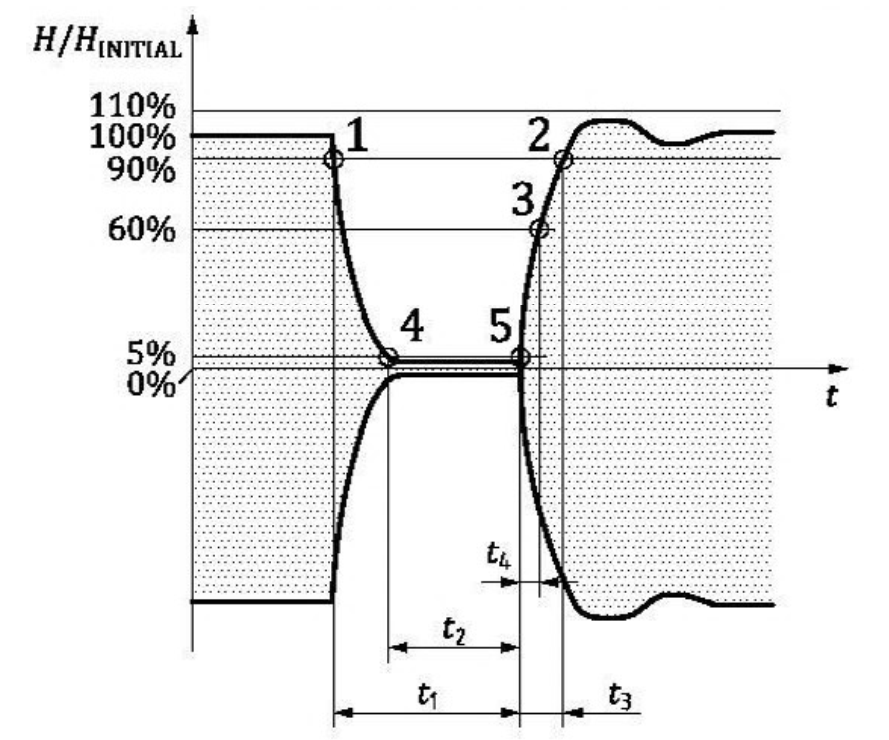
\includegraphics[scale=0.6]{./img/pause}
  \caption{El formato de una pausa tipo A~\cite{iso14443-2}}
  \label{fig:pause}
\end{figure}

\begin{table}[htb]
\centering
\begin{tabular}{|c|c|c|c|}
  \hline
  \textbf{Parámetro} & \textbf{Condición} & \textbf{Mínimo} & \textbf{Máximo} \\
  \hline
  $t_1$                   &                               & $\nicefrac{28}{f_c}$  & $\nicefrac{40,5}{f_c}$    \\
  \multirow{2}{*}{$t_2$}  & $t_1 > \nicefrac{34}{f_c}$  & $\nicefrac{7}{f_c}$   & \multirow{2}{*}{$t_1$}    \\
                          & $t_1 \le \nicefrac{34}{f_c}$  & $\nicefrac{10}{f_c}$  &                           \\
  $t_3$                   &                               & $1,5 \cdot t_4$           & $\nicefrac{16}{f_c}$      \\
  $t_4$                   &                               & 0                     & $\nicefrac{6}{f_c}$       \\
  \hline
\end{tabular}
\caption{Parámetros de timing para una pausa~\cite{iso14443-2}}
\label{tab:pause_values}
\end{table}

\begin{figure}[htb]
  \centering
  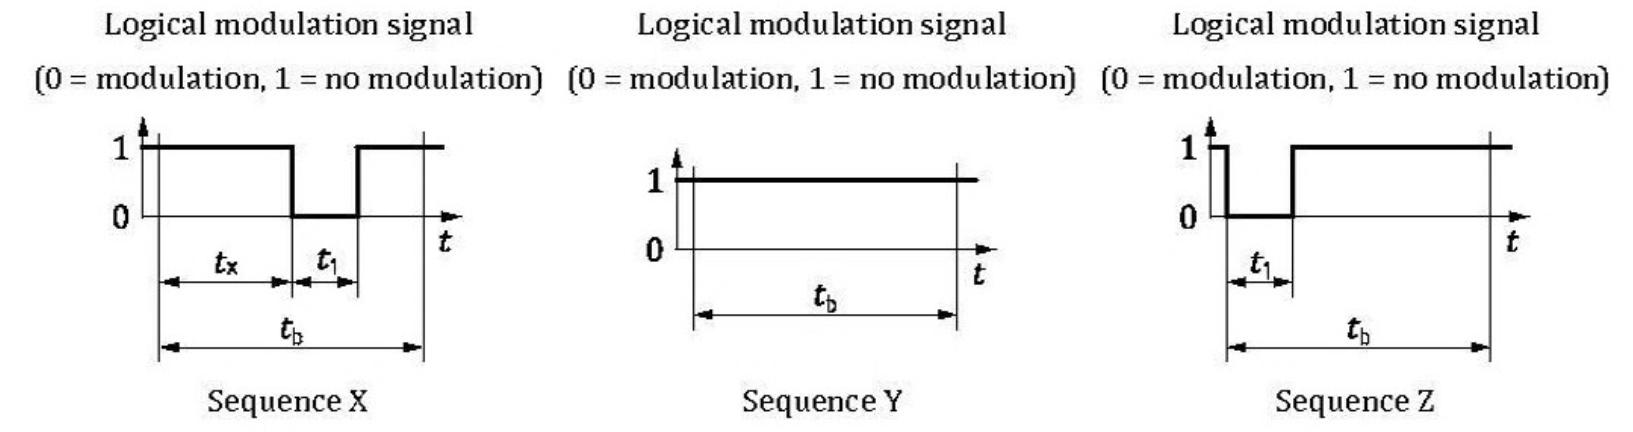
\includegraphics[scale=0.5]{./img/sequences}
  \caption{Codificación Modified Miller~\cite{iso14443-2}}
  \label{fig:sequences}
\end{figure}

\begin{figure}[htb]
  \centering
  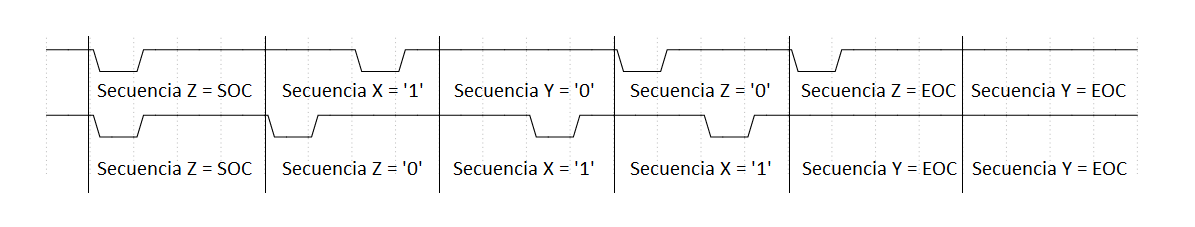
\includegraphics[scale=0.45]{./img/rx_frame_examples}
  \caption{Ejemplos de tramas PCD $\rightarrow$ PICC tipo A}
  \label{fig:rx_frame_examples}
\end{figure}

% There's a lot of images around here, make sure we keep them separated correctly
\FloatBarrier

Para responder las PICCs tipo A usan modulación de carga para generar una subportadora.  La frecuencia de la subportadora ($f_s$) depende de la tasa de bit. Para una tasa de bit de $\nicefrac{f_c}{128}$ la frecuencia de la subportadora es $f_s = \nicefrac{f_c}{16} \approx \SI{848}{\kilo\hertz}$. Como en el caso de comunicaciones del PCD a la PICC la duración de un bit es $\nicefrac{128}{f_c} = \nicefrac{8}{f_s}$. La portadora solo se debe modular con la subportadora cuando la PICC está enviando datos. Los bits a transmitir tienen codificación Manchester, para representar un ‘1’ lógico la señal se mantiene en ‘1’ por la primera mitad de la duración de bit, y en ‘0’ por la segunda mitad, para representar un ‘0’ lógico es al revés. La señal que maneja el modulador de carga es la operación lógica AND entre la señal de codificación Manchester y la subportadora como se muestra en la \figref{fig:picc_to_pcd}. Una trama comienza con un SOC lo que es un ‘1’ lógico, y termina con un EOC lo que es una duración de bit sin modulación, es decir que la señal al modulador de carga está en ‘0’ por toda la duración de bit. La \figref{fig:tx_frame_example} muestra un ejemplo de una trama que ingresa a la compuerta AND con la subportadora.

\begin{figure}[htb]
  \centering
  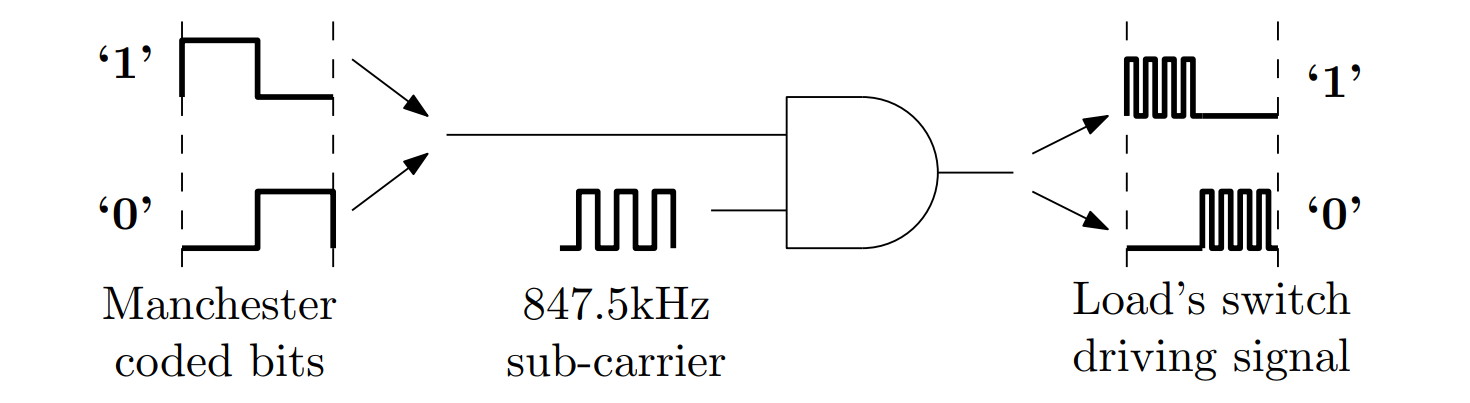
\includegraphics[scale=0.35]{./img/picc_to_pcd}
  \caption{Codificación de bits y modulación de la portadora con la subportadora para comunicaciones de la PICC a PCD~\cite{fabricio_eamta}}
  \label{fig:picc_to_pcd}
\end{figure}

\begin{figure}[htb]
  \centering
  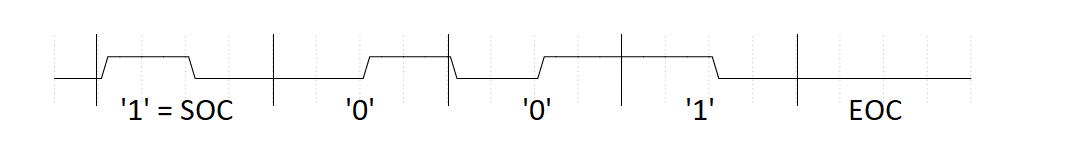
\includegraphics[scale=0.5]{./img/tx_frame_example}
  \caption{Ejemplo de una trama por comunicaciones PICC tipo A $\rightarrow$ PCD.}
  \label{fig:tx_frame_example}
\end{figure}

\FloatBarrier
\subsection{ISO/IEC 14443-3: \large{Inicialización y Anticolisión}}
\label{sec:introduction_iso14443-3}

La información presentada en esta sección es válida considerando una tasa de bit de $\nicefrac{f_c}{128}$ en cada dirección y PICCs tipo A.

La parte 3 de la norma define un FDT (Frame Delay Time), lo que es el tiempo entre dos tramas transmitidas en direcciones opuestas. Los tiempos del FDT definidos en la norma son especificados en números de ciclos de la portadora, y son medidos entre el último flanco de modulación de la primera trama y el primer flanco de modulación de la segunda trama. El \tabref{tab:fdt} muestra los FDTs especificados en la norma. En el caso del FDT entre una trama del PCD y una de la PICC, el FDT usado depende en el último bit lógico de la trama, y los valores especificados son absolutos para tramas de inicialización y tiempos mínimos para otras tramas.

\begin{table}[htb]
  \centering
  \begin{tabular}{|c|c|c|c|}
    \hline
    \textbf{Primera Trama} & \textbf{Segunda Trama} & \textbf{Último Bit} & \textbf{FDT} \\
    \hline
    \multirow{2}{*}{PCD~$\rightarrow$~PICC} & \multirow{2}{*}{PICC~$\rightarrow$~PCD} & '0' & 1172  \\
    \cline{3-4}
    & & '1' & 1236 \\
    \hline
    PICC~$\rightarrow$~PCD & PCD~$\rightarrow$~PICC & & 1272 \\
    \hline
  \end{tabular}
  \caption{Valores del FDT en número de ciclos de la portadora.}
  \label{tab:fdt}
\end{table}

Una trama comienza con un SOC, después se envían los datos empezando por el bit menos significativo, y termina con un EOC. Cada 8 bits de datos hay un bit de paridad impar, así que el número de los 1s en cada byte más su bit de paridad es impar. Hay tres tipos de tramas definidas:

\begin{description}
  \item [Tramas Cortas] \hfill \\ Tienen siete bits de datos sin bit de paridad.
  \item[Tramas Estándares] \hfill \\ Tienen un número de bytes enteros, cada uno con un bit de paridad.
  \item[Tramas Anticolisión orientada a bits] \hfill \\ Tienen siete bytes cada uno con un bit de paridad, y están divididas en dos: la primera parte es enviada desde el PCD y la segunda parte desde la PICC. La partición puede ser después de un byte entero, incluyendo su bit de paridad (\figref{fig:anticollision} arriba), o en medio de un byte (\figref{fig:anticollision} abajo). Estas tramas son usadas durante el proceso de inicialización para que el PCD pueda detectar todas las PICCs en su campo electromagnético.
\end{description}

Unas de las tramas definidas en la norma terminan con un CRC16 (Cyclic Redundancy Check de 16 bits). El CRC16 permite el receptor de la trama determinar si el contenido fue corrompido. El polinomio del CRC es $P\left(x\right) = x^{16} + x^{12} + x^{5} + 1$, y el valor inicial es 0x6363~\cite{iso14443-3}\cite{iso13239}.

Cada PICC tiene un UID (Unique Identifier) que el PCD puede utilizar para enumerar todas las PICCs en su campo electromagnético y elegir cuáles activar. A pesar de que el nombre indique que el ID es único, no tiene que ser así. Está permitido usar un ID aleatorio (RID), o un ID no único (NUID). Los UIDs pueden ser: simples (4 bytes), dobles (7 bytes), o triples (10 bytes). Es requerido que todas las PICCs presentes en el campo de un PCD tienen UIDs únicos. Cuando se usan PICCs con NUIDs o RIDs es posible que haya conflictos. Debido a la gran cantidad de NUIDs posibles, la probabilidad de conflictos es mínima en un sistema bien diseñado.

\begin{figure}[htb]
  \centering
  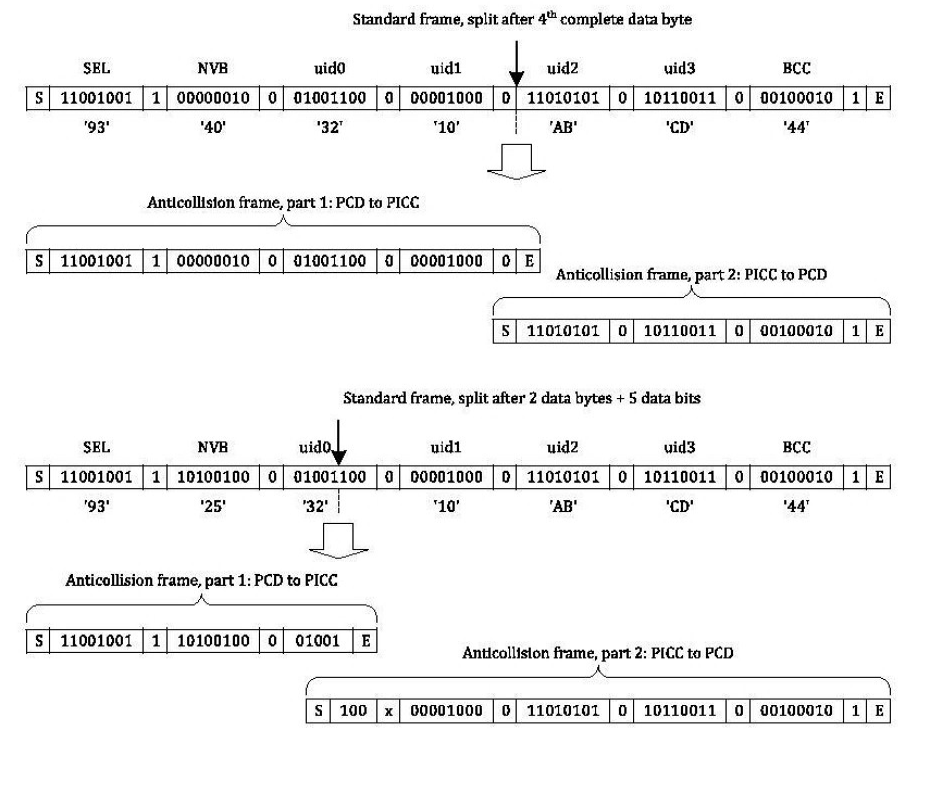
\includegraphics[scale=0.5]{./img/anticollision_frames}
  \caption{Trama Anticolisión orientada a bits~\cite[Adaptado de][]{iso14443-3}}
  \label{fig:anticollision}
\end{figure}

Para identificar las PICCs presentes y activarlas, la norma define cinco comandos y sus respuestas, mostrados en el \tabref{tab:tramas}. La \figref{fig:14443-3-state-machine} especifica cómo una PICC debería responder cuando recibe un comando dependiendo de su estado actual.

\begin{table}[htb]
  \centering
  \begin{tabular}{l l l | l l l}
    \multicolumn{3}{c|}{\textbf{PCD $\rightarrow$ PICC}} & \multicolumn{3}{c}{\textbf{PICC $\rightarrow$ PCD}} \\
    \hline
    \textbf{Solicitud} & \textbf{Tipo} & \textbf{CRC} & \textbf{Respuesta} & \textbf{Tipo} & \textbf{CRC} \\
    \hline
    REQA & Corta & No & ATQA & Estándar & No \\
    WUPA & Corta & No & ATQA & Estándar & No \\
    ANTICOLLISION & Anticolisión & No & ANTICOLLISION & Anticolisión & No \\
    SELECT & Estándar & Sí & SAK & Estándar & Sí \\
    HLTA & Estándar & Sí & Sin Respuesta &  &  \\
  \end{tabular}
  \caption{Solicitudes y respuestas definidas en ISO/IEC 14443-3A}
  \label{tab:tramas}
\end{table}

\begin{figure}[htb]
  \centering
  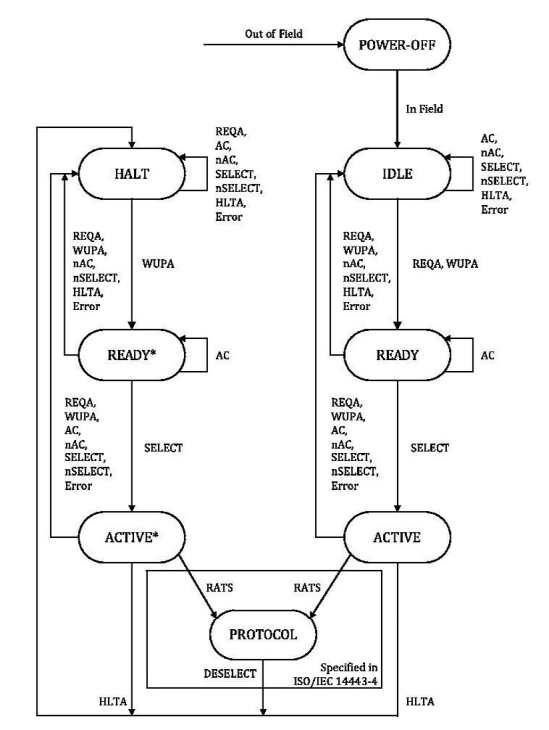
\includegraphics[scale=1]{./img/state_machine}
  \caption{Diagrama de transiciones de estados~\cite{iso14443-3}}
  \label{fig:14443-3-state-machine}
\end{figure}

\FloatBarrier

Cuando una PICC entra en un campo electromagnético, comienza en el estado IDLE. Un comando REQA o WUPA cambia el estado a READY. En ese estado el PCD puede enviar comandos de ANTICOLLISION para determinar el UID de una de las PICCs presentes. Con ese UID el PCD puede enviar un SELECT para mover la PICC al estado ACTIVE. Desde aquí el PCD puede enviar un RATS para terminar activando la PICC. En el caso de recibir un error, o un comando no esperado, la PICC vuelve al estado IDLE. Hay tres otros estados también: HALT, READY* y ACTIVE*. Las diferencias únicas entre estos estados e IDLE, READY y ACTIVE, son: WUPA es el único comando aceptado en HALT y el comando REQA es ignorado, y un error o un comando no esperado recibido en READY* o ACTIVE* causa la PICC volver a HALT en vez de IDLE. La ventaja de esto es que si el PCD decide que no quiere activar una PICC particular, puede ponerla en el estado HALT, y enviando un nuevo REQA comenzará el proceso de inicialización de nuevo en todos las PICCs menos aquellos que están en HALT.

En el caso de una PICC con UID doble el proceso de ANTICOLLISION y SELECT tiene que repetir dos veces antes de que la PICC se mueva al estado ACTIVE. En el primer lazo, los mensajes usan los primeros tres bytes de su UID junto con una etiqueta cascada: CT (Cascade Tag). La PICC responde al SELECT especificando que su UID no está completo todavía, y el lazo comienza de nuevo, esta vez usando los últimos cuatro bytes del UID. Por una PICC con UID triple este proceso tiene tres lazos. La \figref{fig:cascade_levels} muestra este proceso.

\begin{figure}[htb]
  \centering
  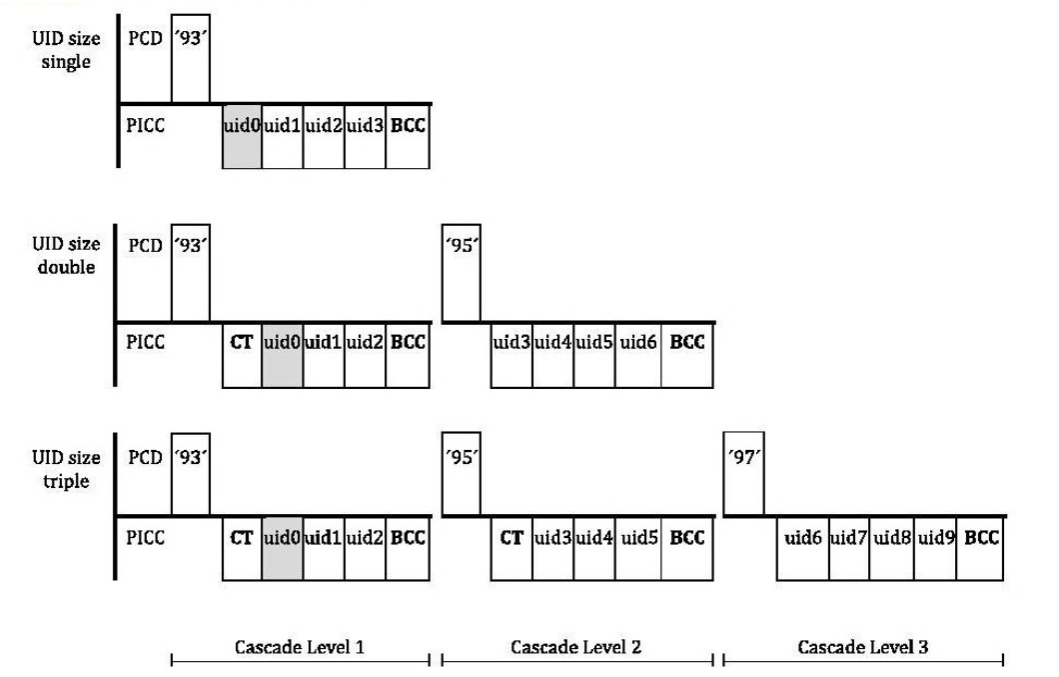
\includegraphics[scale=0.75]{./img/cascade_levels}
  \caption{Niveles cascadas para UIDs simples, dobles y triples~\cite{iso14443-3}}
  \label{fig:cascade_levels}
\end{figure}

El comando de ANTICOLLISION funciona de la siguiente forma: el PCD envía un UID parcial, y todas las PICCs en el campo electromagnético cuyas UIDs corresponden con la parte enviada, responden con los demás bits de sus UIDs. Debido al FDT fijo todas las PICCs comienzan responder de forma sincronizada. Las respuestas tienen codificación Manchester, por lo tanto cuándo dos PICCs envían valores lógicos diferentes el PCD puede detectar la colisión porque hay modulación durante todo el tiempo de bit. De esta manera el PCD sabe qué parte del UID es compartido entre todas las PICCs, y usando una búsqueda binaria puede determinar el UID completo de una de las PICC presentes. Esa PICC entonces puede ser activada o puesta en el estado HALT, y después el PCD puede repetir el proceso para enumerar todas las demás PICCs.

\FloatBarrier
\subsection{ISO/IEC 14443-4: \large{Protocolo de Transmisión}}

La mayor parte de esta subsección es común para PICCs tipo A y B, sin embargo hay dos comandos extras para terminar activando el protocolo para PICCs de tipo A. Estos comandos son RATS y PPS. El PCD debería enviar un RATS como el primer comando después de que una PICC entra en el estado ACTIVE o ACTIVE*. En el RATS el PCD asigna un CID (Card Identifier) a la PICC, esto es un identificador que el PCD puede usar para direccionar un mensaje a una PICC en particular, así que el CID debe ser único para cada PICC activa. En diferencia al UID, el CID solo tiene cuatro bits y son asignados  al momento de la inicialización y no en la  de fabricación. Este CID es válido sólo hasta que la PICC es desactivada. La respuesta al RATS es la ATS lo que contiene información sobre la capacidad de la PICC, por ejemplo las tasas de bits y el tamaño máximo de una trama que la PICC puede recibir. El comando PPS es opcional, y solo puede ser enviado inmediatamente después de que el PCD recibe la ATS. El PPS permite al PCD configurar las tasas de bits de comunicaciones en cada dirección.

La norma define dos formatos de bloques: estándares y aumentados. Bloques estándares están enviados en tramas estándares con el CRC16 presente. Bloques aumentados comienzan con el largo del bloque, y terminan con un CRC32, y el campo INF contiene códigos Hammings para la corrección de errores. La \figref{fig:std_enhanced_blocks} muestra los dos. Comunicaciones comienza con bloques estándares hasta que el PCD configura lo contrario.

\begin{figure}[htb]
  \centering
  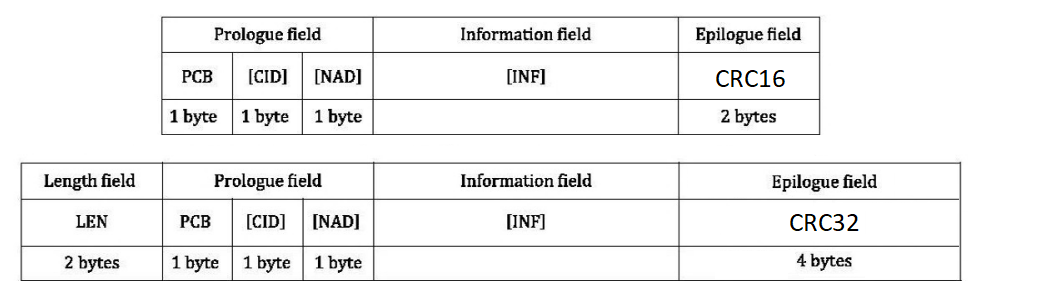
\includegraphics[scale=0.52]{./img/bloque_formats}
  \caption{El formato de un bloque estándar (arriba) y uno aumentado (abajo)~\cite{iso14443-4}}
  \label{fig:std_enhanced_blocks}
\end{figure}

Hay tres tipos de bloques: I (Information), R (Receive Ready) y S (Supervisory). El campo PCB indica que tipo de bloque es. El CID es la dirección de la PICC y solo está presente si la PICC lo soporta. El campo CID en respuestas también contiene dos bits con información sobre el nivel de potencia recibido, el PCD puede usar esa información para controlar la potencia transmitida por el campo. La NAD (Node Address) permite una PICC tener más de una aplicación, direccionado por este campo, también solo está presente si la PICC la soporta. Finalmente el campo INF contiene la información del bloque, y solo está presente en bloques tipos I y S.

Bloques-S son usados para información de control. Hay tres comandos definidos:

\begin{description}
  \item[S(WTX)] \hfill \\ Waiting Time eXtension. Si la PICC no está lista para responder a una solicitud en el tiempo permitido, puede responder con un S(WTX) pidiendo más tiempo.
  \item[S(DESELCT)] \hfill \\ Este comando es enviado por el PCD cuándo quiere desactivar la PICC.
  \item[S(PARAMETERS)] \hfill \\ Este comando está usado para leer o setear la configuración de la PICC. Por ejemplo, para cambiar la tasa de bits, o cambiar entre bloques estándares y aumentados.
\end{description}

Bloques-I son usados para transmitir información al nivel de aplicación. El protocolo de la aplicación no está definido en esta norma. Estos bloques pueden ser encadenados para permitir el envío de un mensaje más grande que el soportado por el destino, partiendo el mensaje en partes de tamaños soportados.

Bloques-R son usados para reconocer la recepción de un bloque: R(ACK) o indicar errores: R(NAK). En el caso de bloques-I encadenados un R(ACK) es enviado para pedir la siguiente parte del mensaje. También el PCD puede enviar un R(ACK/NAK) para pedir la PICC retransmita su última respuesta, esto puede ser usado para recuperar tramas con errores. Finalmente el PCD puede enviar un R(NAK) para verificar la presencia continua de la PICC.

% ---------------------------------------------
% Descripción del Proyecto Marco
% ---------------------------------------------

\FloatBarrier
\chapter{Descripción del Proyecto Marco}

Este trabajo se enmarca en un proyecto que tiene como objetivo general desarrollar un circuito integrado capaz de tomar muestras de un sensor MOSFET de radiación y transmitirlas a un dispositivo externo mediante un protocolo propietario implementado encima de la norma ISO/IEC 14443A. Este proyecto marco requiere cinco bloques como se muestra en la \figref{fig:entire_project}:

\begin{figure}[htb]
  \centering
  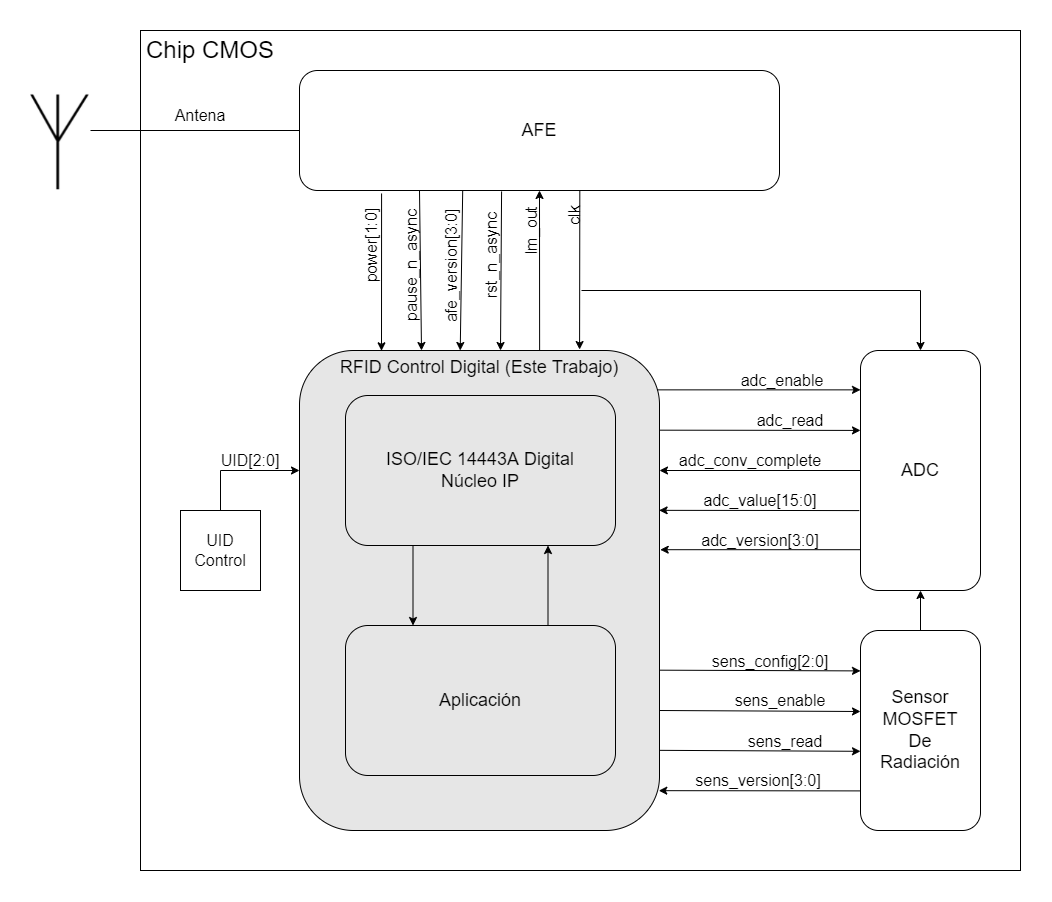
\includegraphics[width=0.95\textwidth]{./img/entire_project_v2}
  \caption{Diagrama general del proyecto marco y su relación con el bloque a diseñar en esta Tesis.}
  \label{fig:entire_project}
\end{figure}

\begin{description}
  \item[El Analogue Front End (AFE)] \hfill \\ Es la parte analógica de la norma ISO/IEC 14443A-2.
  \item[El sensor MOSFET de radiación] \hfill \\ Desarrollado por el Laboratorio de Física de Dispositivos-Microelectrónica (LFDM) de la Facultad de Ingeniería de la UBA~\cite{Lipovetzky_2013}\cite{mosfet_mismatch_amplification}\cite{6MV_LINAC}. El sensor es un transistor MOS de óxido grueso completamente compatible con el proceso de fabricación CMOS. Su elevado espesor de óxido ($\sim$40 veces mayor al nativo) permite obtener una sensibilidad adecuada para radioterapia y al mismo tiempo puede integrarse en el chip con otros circuitos. Durante la exposición a radiación ionizante todos los transistores del chip reciben la misma dosis de radiación, pero  los efectos sobre los transistores nativos del proceso de espesor de óxido regular son despreciables en el rango correspondiente a la aplicación~\cite{Saks_1984}.
  \item[El Conversor Analógico Digital (ADC, por sus siglas en inglés)] \hfill \\ Encargado de convertir la salida analógica del sensor a una señal digital.
  \item[El RFID Control Digital] \hfill \\ Es el objetivo de esta Tesis.
  \item[El UID Control] \hfill \\ Permite asignar la parte única del UID de la PICC.
\end{description}

Algunos de estos bloques no se han desarrollado todavía, por lo que es necesario asumir las especificaciones de los mismos.

El AFE es responsable de:

\begin{itemize}
  \item Recibir y regular potencia desde el campo electromagnético. La implementación de esta tesis se realiza considerando la tecnología de fabricación de XFAB 180 nm, la cual utiliza celdas estándares que requieren una tensión de 1.8 V, por lo que el AFE debe producir esa tensión, y mantenerla durante las pausas.
  \item Recuperar la señal de reloj a partir de la portadora. La dificultad en este punto reside en el hecho de que el PCD envía información a la PICC utilizando pausas en la portadora, por lo cual se espera que el reloj se detenga durante estas pausas. Es posible utilizar un PLL para producir un reloj continuo. El circuito de esta tesis es elaborado con habilidad para funcionar con un reloj continuo o con un reloj que se detenga durante las pausas. En la \secref{sec:sequence_decode}{sequence\_decode} se detalla el número máximo de flancos del reloj que es posible perder conservando una correcta decodificación de las secuencias.
  \item Manejar la señal de reset (activa baja). Los demás bloques se deben mantener en un estado de reset hasta que la tensión de alimentación sea estable.
  \item Detectar las pausas enviadas desde el PCD.
  \item Permitir la transmisión de respuestas al PCD mediante un modulador de carga. El modulador debería ser manejado directamente desde una entrada del bloque, lo cual sería conectado a la salida \textit{lm\_out} del bloque RFID Digital Control. La señal se obtiene como el AND lógico de la codificación Manchester y la subportadora.
  \item Generar una señal indicando el nivel de potencia recibida a través del campo electromagnético (opcional). Si se tiene esta información, la misma puede ser enviada al PCD en el campo CID de mensajes de nivel protocolo. El PCD puede usarla para ajustar la intensidad del campo electromagnético.
  \item Proveer una salida de cuatro bits que indique la versión del hardware del AFE. Este valor forma parte de la información enviada al PCD como respuesta al mensaje de protocolo IDENTIFY.
\end{itemize}

El sensor de radiación tiene tres entradas: \textit{sens\_config[2:0]}, \textit{sens\_enable} y \textit{sens\_read} . Para leer el sensor, primero se debe establecer el valor de \textit{sens\_config[2:0]} de manera que se elija la configuración del sensor deseado por el usuario. Posteriormente se debe establecer \textit{sens\_enable} en ‘1’ para activar el sensor. Finalmente después del tiempo deseado por el usuario, llevar \textit{sens\_read} a ‘1’ configura al circuito del sensor en modo lectura para su muestreo. Por otro lado, el sensor tiene dos salidas, una analógica que está conectada al ADC, y una señal de cuatro bits que indica la versión del sensor. Este valor forma parte de la información enviada al PCD como respuesta al mensaje de protocolo IDENTIFY.

Por su parte el ADC, además de la entrada analógica proveniente desde el sensor, tiene otras dos entradas: \textit{adc\_enable} y \textit{adc\_read}. El flanco ascendente de la señal \textit{adc\_read} indica el momento de muestreo de la salida del sensor. Respecto de las salidas, hay tres: \textit{adc\_conversion\_complete}, \textit{adc\_value[15:0]} y \textit{adc\_versión[3:0]}. Cuando el ADC completa la conversión la señal \textit{adc\_conversion\_complete} toma el valor '1' durante un ciclo del reloj. La señal \textit{adc\_value} debe ser estable antes del pulso en \textit{adc\_conversion\_complete}.

El bloque de UID Control es responsable de especificar los tres bits menos significativos del UID de la PICC. Este valor puede ser configurado mediante una memoria no volátil, pero en esta tesis la intención es configurarlo utilizando wire bonding o resistores pull up/down.

El objetivo de esta tesis es implementar el bloque del RFID Control Digital, que consiste en dos sub-bloques: Una implementación del parte digital de la norma ISO/IEC 14443A y un protocolo a nivel aplicación que permita la lectura del sensor y envíe esta información al PCD. Un requisito de este bloque es que la entrada de UID se mantenga estable mientras el bloque no esté en un estado de reset.

% --------------------------------------------
% Implementación y Verificación
% ---------------------------------------------

\FloatBarrier
\chapter{Implementación y Verificación}

La implementación de todos los módulos y los bancos de prueba se escriben con el HDL (Hardware Description Language) SystemVerilog, el cual  es definido en IEEE 1800~\cite{ieee1800}. SystemVerilog es basado en Verilog,  formalmente definido en IEEE 1364~\cite{ieee1364}. SystemVerilog es conocido principalmente como un HDL para verificación debido a sus extensiones sustanciales a verilog en ese ámbito, por ejemplo en la adición de conceptos de programación orientados a objetivos (como clases), y aserciones. Además SystemVerilog tiene varias ventajas a Verilog para uso en síntesis~\cite{synthesisable_sv}, por ejemplo:

\begin{description}
  \item[Enumeraciones (enum) y estructuras (struct)] \hfill \\ Como en el lenguaje de programación C.
  \item[always\_comb y always\_ff] \hfill \\ Estos permiten al ingeniero especificar su intención a implementar lógica combinatoria o secuencial respectivamente. Las herramientas pueden verificar que el circuito inferido cumple con esa intención, por ejemplo, que los bloques combinatorios no contienen latches.
  \item[Interfaces] \hfill \\ Colecciones de señales que son frecuentemente usadas juntas para reducir la replicación de código.
\end{description}

La implementación de esta tesis está dividida en dos: 1) El núcleo IP genérico para ISO/IEC 14443A que es la lógica digital necesaria para recibir, decodificar y actuar sobre los mensajes definidos en la norma, y construir, codificar y transmitir las respuestas adecuadas. Este núcleo IP está dividido en tres partes principales, uno para cada parte de la norma (excepto ISO/IEC 14443-1). 2) El sistema de control del sensor y del ADC. La \figref{fig:top_level} muestra todos esos bloques, y el flujo de datos entre ellos.

\begin{figure}[htb]
  \centering
  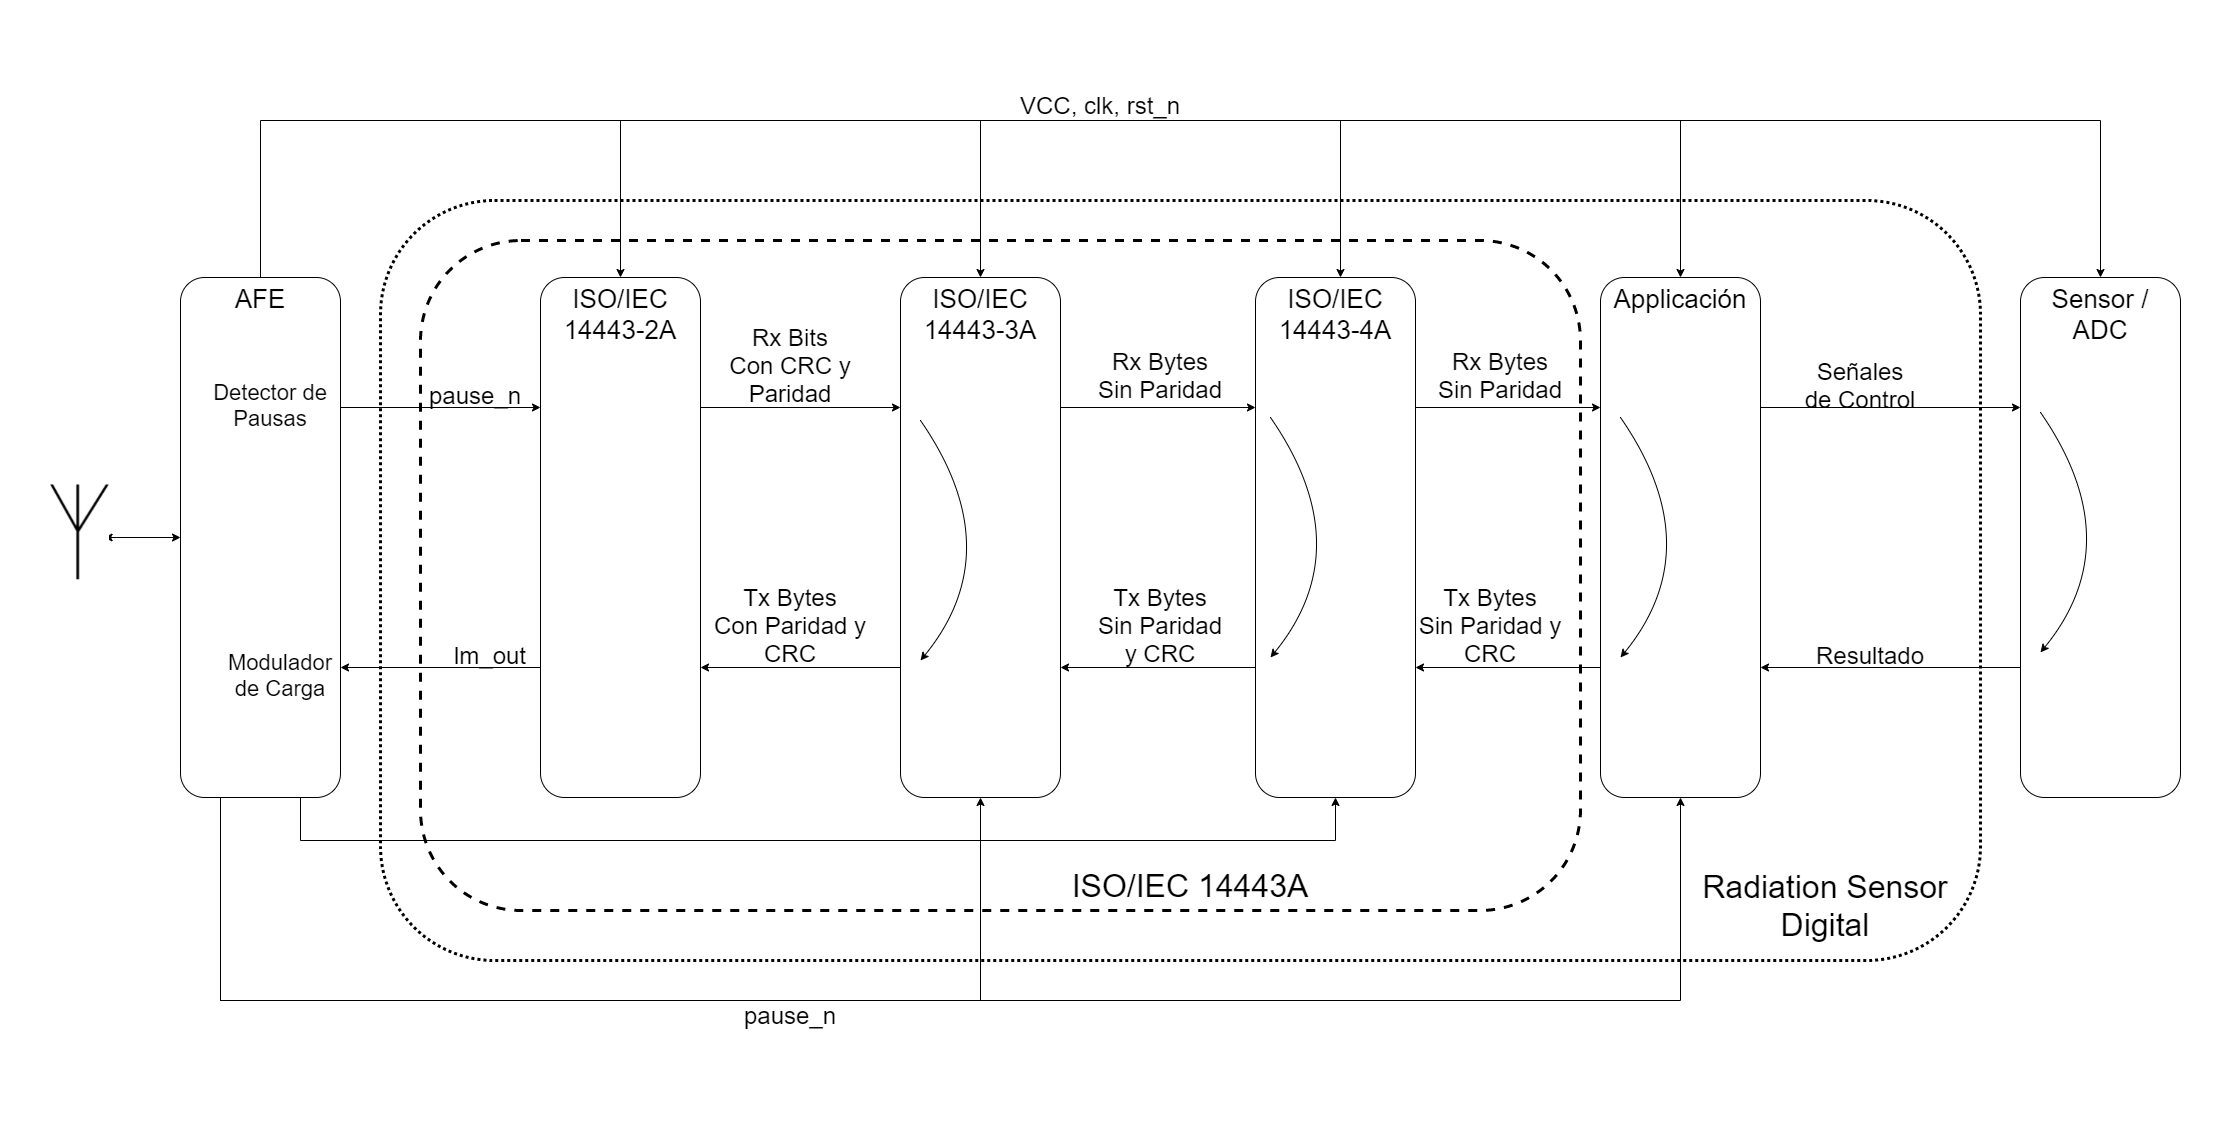
\includegraphics[width=1.0\textwidth]{./img/top_level}
  \caption{Los bloques principales de la implementación.}
  \label{fig:top_level}
\end{figure}

% Interfaces
% --------------------------------
\FloatBarrier
\section{Interfaces}

La norma IEEE de SystemVerilog define un interfaz como:

\begin{displaycquote}[traducido de][]{ieee1800}
A su nivel más bajo, un interfaz es un conjunto nombrado de nets o variables. La interfaz es instanciada en un diseño y puede ser accedida por un puerto como un ítem sencillo; las nets o variables componentes [pueden ser] referidos cuando sea necesario. Una proporción significativa de un diseño verilog frecuentemente consiste en listas de puertos y listas de conexiones, los que son simplemente repeticiones de nombres. La habilidad de reemplazar un grupo de nombres con un nombre simple puede reducir significativamente el tamaño de una descripción y mejorar su mantenibilidad.
\end{displaycquote}

Además de esas ventajas, una interfaz puede contener funcionalidad, sea para síntesis o verificación, por ejemplo se puede agregar aserciones que verifican el comportamiento de los nets internos en vez de tener que duplicar esas pruebas en cada sitio que la interfaz es usada. Una interfaz puede tener uno o más modports, los que especifican las direcciones de las señales. Esos modports pueden ser usados en la lista de puertos por un módulo en vez de especificar cada señal y su dirección individualmente.

Este trabajo consiste en varios módulos que contienen uno o más sumideros para recibir tramas desde otros módulos, y una o más fuentes para enviar tramas a otros módulos. Por ejemplo el módulo: \textbf{frame\_decode} recibe tramas desde el módulo: \textbf{sequence\_decode}, quita los bits de paridad, y reenvía las tramas modificadas al módulo: \textbf{deserialiser}. Por lo tanto muchos de los módulos manejan el mismo conjunto de señales, lo que es el uso principal por interfaces. Hay dos interfaces definidas en este trabajo, uno para la recepción de tramas (\textit{rx\_interface}), y otra para la transmisión de las respuestas (\textit{tx\_interface}). Las dos son parametrizadas para funcionar con series de bits o de bytes. Las interfaces son usadas para conectar una fuente en un módulo a un sumidero en otro módulo.

La \textit{rx\_interface} contiene:

\begin{itemize}
  \item \textit{soc}: Un indicador que indica el comienzo de una trama.
  \item \textit{eoc}: Un indicador que indica el fin de una trama.
  \item \textit{data}: Un bit / byte de la trama.
  \item \textit{data\_valid}: Un indicador que indica si los datos en \textit{data} son válidos.
  \item \textit{data\_bits}: La cantidad de bits válidos. Por una interfaz configurada a bytes, esta señal permite la recepción de tramas cortas que tienen solo 7 bits, o de tramas anticolisión orientada a bits que pueden terminar con entre uno y ocho bits.
  \item \textit{error}: Indica la detección de un error en la trama, por ejemplo: un bit de paridad equivocado.
\end{itemize}


La \figref{fig:rx_iface} muestra una simulación de la recepción de una trama corta con una \textit{rx\_interface} de bits, y su conversión a una serie de bytes. Arriba están las señales en una \textit{rx\_interface} de bits, \textit{data\_valid} está en ‘1’ siete veces durante la trama, indicando que el dato recibido es: 1,1,1,1,0,1,0. Debido a que el bit menos significativo es enviado primero, este serie representa 7’b0101111. Abajo están las señales en una \textit{rx\_interface} de bytes representando la misma trama. El dato tiene valor 8’bX0101111 cuando \textit{data\_valid} tiene valor lógico igual a ‘1’.

La \textit{rx\_interface} incluye varias aserciones para verificar el comportamiento de las señales en la interfaz. Las aserciones consideran: Las señales son correctas en el estado de reset, los indicadores nunca son desconocidos, \textit{soc} y \textit{eoc} no están en ‘1’ en el mismo ciclo, y que solo están en ‘1’ por la duración de un solo ciclo del reloj a la vez.

\begin{figure}[htb]
  \centering
  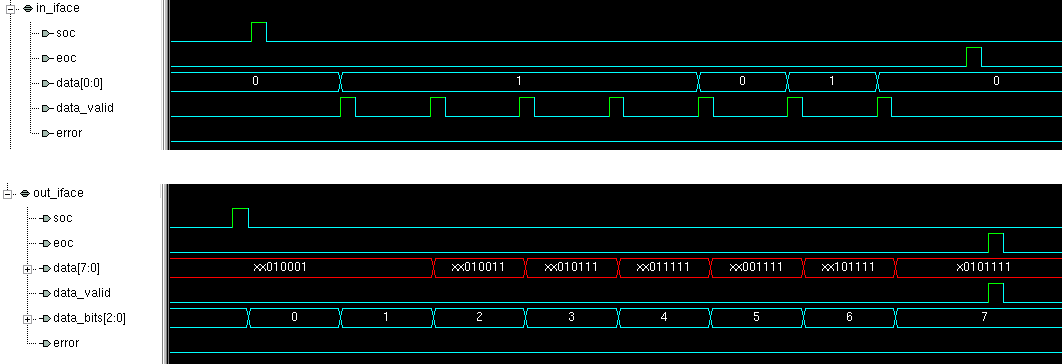
\includegraphics[width=1.0\textwidth]{./img/rx_iface_example}
  \caption{Una simulación de la recepción de una trama corta representada con una \textit{rx\_interface} de bits (arriba) y su conversión a una \textit{rx\_interface} de bytes (abajo).}
  \label{fig:rx_iface}
\end{figure}

\FloatBarrier

La \textit{tx\_interface} contiene:

\begin{itemize}
  \item \textit{data}: Un bit / byte de la trama.
  \item \textit{data\_valid}: Un indicador que indica que \textit{data} es válida.
  \item \textit{data\_bits}: La cantidad de bits válidos. Para una interfaz configurada a bytes, esta señal permite la transmisión de tramas de anticolisión orientada a bits, las que pueden comenzar con un byte parcial.
  \item \textit{last\_bit\_in\_byte}: Esta señal solo existe en interfaces de bits. Indica que el bit actual es el último bit en un byte. Es usada para conocer dónde agregar bits de paridad dentro de una serie de bits.
  \item \textit{req}: El sumidero usa esta señal para pedir que la fuente envíe el siguiente bit / byte de la trama. La norma ISO/IEC 14443A-2 define la duración de bits como 128 ciclos de la portadora, por lo tanto esta señal es necesaria para limitar la tasa de envío de datos.
\end{itemize}

Cuando una fuente está lista para transmitir una trama se establece el primer bit / byte de la trama en la señal \textit{data} y fija \textit{data\_valid} en ‘1’. El sumidero puede utilizar la señal \textit{data\_valid} para ver si la fuente tiene datos para enviar. Después de haber leído la primera bit~/~byte de data, el sumidero fija la señal \textit{req} en ‘1’ durante un ciclo del reloj. La fuente detecta ese pulso y si hay más datos a enviar, se actualiza la \textit{data} con el siguiente bit / byte, dejando \textit{data\_valid} en ‘1’. Este proceso repite hasta que la fuente no tiene más datos a enviar, y después del último pulso en la \textit{req}, se fija \textit{data\_valid} en ‘0’. La \figref{fig:tx_iface} muestra una simulación de la transmisión de una trama de 16 bits con una \textit{tx\_interface} de bytes, y su conversión a una serie de bits. Arriba están las señales en la \textit{tx\_interface} de bytes enviando la data 0xAE, 0x42. Abajo están las señales en una \textit{tx\_interface} de bits representando la misma trama.

La \textit{tx\_interface} también incluye tres aserciones que verifican: Las señales son correctas en el estado de reset, \textit{req} es ‘1’ solo para la duración de un ciclo del reloj, y que \textit{data}, \textit{data\_valid}, \textit{data\_bits} y \textit{last\_bit\_in\_byte} solo cambian estado cuando \textit{data\_valid} está ‘0’ o en los cuatro ciclos después de un pulso de req. La última aserción es para verificar que la fuente puede proveer datos cuándo es pedido con la señal \textit{req} antes de que el sumidero la necesita.

\begin{figure}[htb]
  \centering
  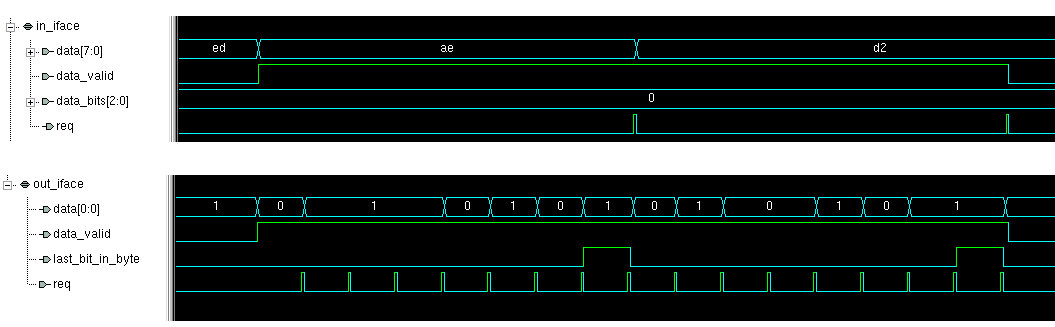
\includegraphics[width=1.0\textwidth]{./img/tx_iface_example}
  \caption{Una simulación de la transmisión de una trama de 16 bits representada con una \textit{tx\_interface} de bytes (arriba) y su conversión a una \textit{tx\_interface} de bits (abajo).}
  \label{fig:tx_iface}
\end{figure}


% Marco de Verificación
% --------------------------------
\FloatBarrier
\section{Marco de Verificación}

Simulación y verificación son una parte muy importante del diseño digital. En un informe de 2020 sobre las tendencias de diseño y verificación de ICs y ASICs~\cite{verification_trends_2020}, los autores encontraron que en promedio más de 50\% del tiempo de un proyecto es utilizado en verificación. También encontraron que en promedio hay un ingeniero de verificación por cada ingeniero de diseño, además los ingenieros de diseño gastan aproximadamente la mitad de su tiempo verificando sus diseños.

En esta tesis se utiliza verificación funcional mediante simulaciones con la herramienta VCS de Synopsys. Las simulaciones son completamente automatizadas y son ejecutadas con un comando sencillo utilizando un Makefile, por ejemplo: “make serialiser\_tb”.

UVM (Universal Verification Methodology) es una metodología de verificación funcional mediante un conjunto de clases de SystemVerilog. Aproximadamente 75\% de proyectos mundiales son verificados con UVM~\cite{verification_trends_2020}. Una de las ventajas principales de UVM es la modularidad. El código es partido en bloques separados facilitando la reutilización de los componentes en varios bancos de pruebas sin tener que duplicar código. La desventaja principal es la complejidad, requiere mucho código para armar un banco de prueba. UVM no es usada en esta tesis porque su implementación sería más compleja que el propio diseño. Sin embargo el marco de verificación está basado en las técnicas de UVM.

El proceso de verificación es estimular las entradas del DUT (Design Under Test) y verificar que las salidas son las esperadas. Frecuentemente no es posible verificar un diseño para todas las combinaciones y secuencias posibles de las entradas, por lo tanto es común usar estímulo aleatorio. Con estímulo aleatorio siempre hay el riesgo de no verificar parte del diseño, por la posibilidad de no elegir una de las combinaciones o secuencias de entradas necesarias para estimular esa parte del diseño. Una técnica para ayudar a mitigar esto, es: aleatorio restringido (constrained random), esta técnica permite la generación de estímulo aleatorio mediante constraints para restringir el estímulo a un rango interesante en particular. Por ejemplo, en vez de generar tramas completamente aleatorias, pueden ser limitadas: a tramas válidas, una colección de tramas en particular, o tramas con errores.

Una técnica para asegurar que todas las partes de un diseño son verificadas suficientemente, es generar informes de cobertura. La herramienta VCS está habilitada para generar, de forma automática, informes de cobertura de código con varias métricas, y un resultado total de qué proporción del diseño fue verificado. Estos informes pueden ser analizados por el diseñador para verificar cuáles partes de su diseño fue suficientemente estimulado y cuáles partes necesitan más trabajo. Las métricas de cobertura de código habilitadas en VCS son:

\begin{itemize}
  \item Línea: Muestra las líneas del RTL que fueron ejecutadas.
  \item Condición: Muestra las sub expresiones booleanas que fueron evaluados a verdadero y falso. Por ejemplo en la declaración: “res = (A == 0) ? B : C”, el informe de cobertura indicará si la expresión “A == 0” fue evaluado al menos una vez a verdadero y al menos una vez a falso.
  \item Cambio de Estado (Toggle): Muestra cuáles señales y puertos cambiaron de estado en las dos direcciones.
  \item Branch: Muestra cuáles branches fueron tomados.
  \item FSM (Finite State Machine): Muestra cuáles estados en un FSM fueron utilizados, y las transiciones entre ellos.
  \item Aserción: Muestra cuáles aserciones fueron: ejecutadas, aprobadas y falladas, y cuántas veces por cada uno.
\end{itemize}

El marco de verificación es implementado con varios componentes, la mayoría son clases de SystemVerilog. Los componentes pueden ser divididos en siete grupos distintos:

\begin{itemize}
  \item Transacciones: Una transacción representa una trama, puede ser una trama de bits, de bytes o de secuencias (como definido en ISO/IEC 14443-2).
  \item Controladores: Un controlador envía una transacción sobre una interfaz.
  \item Monitores: Un monitor monitoriza una interfaz, y construye transacciones representando las tramas detectadas.
  \item Generador de transacciones: Genera transacciones de bytes para representar las tramas definidas en la norma. También puede generar transacciones aleatoriamente.
  \item Convertidor de transacciones: Produce una transacción en un formato desde una transacción en otro formato. Por ejemplo puede convertir una transacción de bytes a una transacción de bits, opcionalmente agregando los bits de paridad.
  \item Secuencias: Código compartido para verificar diseños que reciben tramas, actúan sobre ellos, y generan las respuestas. Por ejemplo: cuándo el DUT está en el estado READY, responde a un SELECT con un SAK con los valores esperados, y se transiciona al estado ACTIVE. Ese ejemplo es una prueba utilizada para verificar el comportamiento de cuatro módulos: \textbf{initialization}, \textbf{iso14443\_3a}, \textbf{iso14443a}, \textbf{radiation\_sensor\_digital\_top}.
  \item Otros: Este grupo incluye: modelos de los bloques analógicos, una clase para guardar la dirección de una PICC (UID, CID y NAD), y unas interfaces que solo están usadas para verificación.
\end{itemize}

% Transacciones
\FloatBarrier
\subsection{Transacciones}

La \figref{fig:transaction_uml} muestra un diagrama UML (Unified Modelling Language) de las clases de transacciones. La clase base es \textbf{Transaction}, es abstracta y contiene dos métodos abstractos: \textbf{compare()} que evalúa si dos transacciones son iguales, y \textbf{to\_string()} que devuelve un string describiendo la transacción. La clase \textbf{QueueTransaction} extiende \textbf{Transaction}, tiene un parámetro de tipo: \textit{ElemType}, que especifica el tipo de una cola declarada en la clase. La cola es usada para contener los datos de la trama representada por la transacción. Los dos métodos abstractos de \textbf{Transaction} son sustituidos, y hay métodos extras para ayudar con la construcción de transacciones. Hay tres clases que extienden \textbf{QueueTransaction}: \textbf{ByteQueueTransaction}, \textbf{BitQueueTransaction} y \textbf{PCDPauseNTransaction}, que definen el parámetro \textit{ElemType} como: logic[7:0] (byte), logic (bit) y \textbf{PCDBitSequence} respectivamente. \textbf{PCDBitSequence} es una enum definida en un paquete, y consiste en las secuencias X, Y y Z describidas en la \secref{sec:introduction_iso14443-2}{ISO/IEC 14443-2}. \textbf{ByteQueueTransaction} tiene métodos para calcular y agregar CRCs a la transacción, y para convertir la transacción a una cola de bits. \textbf{BitQueueTransaction} tiene un método para agregar los bits de paridad.

\begin{figure}[htb]
  \centering
  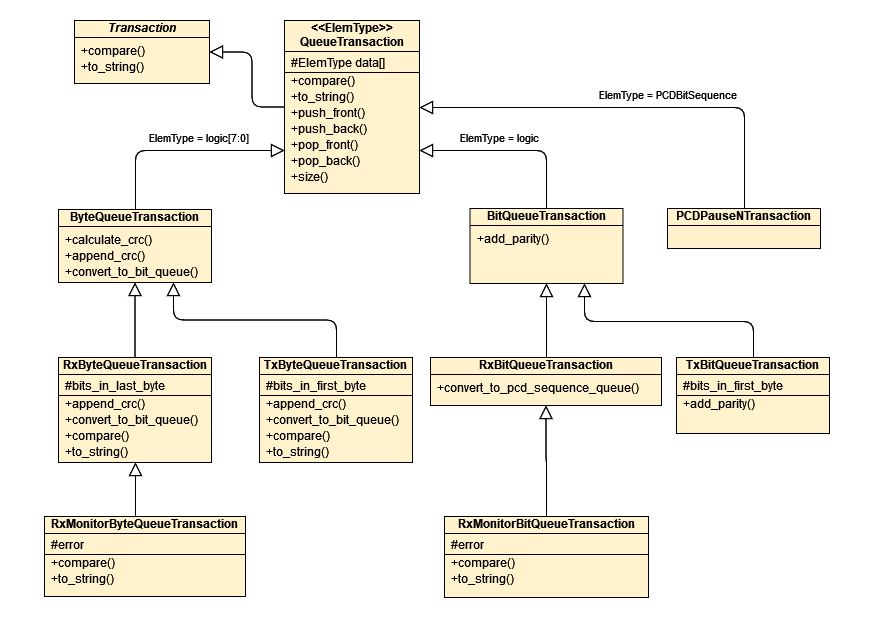
\includegraphics[width=1.0\textwidth]{./img/transactions_uml.vpd}
  \caption{Diagrama UML de clases de transacciones.}
  \label{fig:transaction_uml}
\end{figure}

Para transacciones de transmisión (PICC a PCD), hay dos clases \textbf{TxByteQueueTransaction} y \textbf{TxBitQueueTransaction}, las dos tienen un atributo especificando cuántos bits hay en el primer byte, eso es porque respuestas a mensajes de ANTICOLISIÓN pueden comenzar con un byte parcial, como se muestra en la \figref{fig:anticollision}.

Para transacciones de recepción (PCD a PICC), hay cuatro clases en adición a \textbf{PCDPauseNTransaction}: \textbf{RxByteQueueTransaction}, que tiene un atributo especificando cuántos bits hay en el último byte para tramas cortas y de anticolisiones que pueden terminar con un byte parcial. \textbf{RxBitQueueTransaction}, que tiene un método para convertir su data a una cola de \textbf{PCDBitSecuences}. Estas dos clases son usadas en los controladores para enviar transacciones a los DUTs. Las otras dos clases son \textbf{RxMonitorByteQueueTransaction} y \textbf{RxMonitorBitQueueTransaction}, las que son son las transacciones construidos por los Monitores de recepción. Los dos tienen un atributo para indicar si el monitor ha detectado un pulso en la señal \textit{error} de las interfaces de recepción.

% Controladores
\FloatBarrier
\subsection{Controladores}

La \figref{fig:driver_uml} muestra un diagrama UML de clases para los controladores. La clase base principal es \textbf{Driver}, es abstracta y tiene dos tipos parametrizados: \textit{IfaceType}, que es el tipo de la interfaz que maneja, y \textit{TransType}, que es el tipo de las transacciones que el controlador puede envíar sobre esa interfaz. El método \textbf{start()} lleva una referencia a una cola de elementos de tipo \textbf{TransType} y comienza un nuevo hilo de ejecución. Ese hilo monitoriza la cola, cuándo una transacción es empujada a la cola desde el banco de prueba, la controladora la quita, y la pasa al método \textbf{process()}. En esta clase base \textbf{process()} es abstracto, las clases hijas lo sustituyen para definir cómo envíar la transacción sobre su interfaz.

\textbf{RxIfaceDriver} es la clase base para los controladores de las interfaces de recepción (PCD a PICC). \textbf{RxByteIfaceDriver} y \textbf{RxBitIfaceDriver} la extienden para uso con las interfaces de bytes y de bits respectivamente. Las implementaciones del método \textbf{process()} envían el SOC, los datos y el EOC. Esas clases tienen atributos para controlar el timing de las transmisiones, por ejemplo el tiempo entre el SOC y el primer dato, y entre los datos mismos. También esas clases pueden introducir errores en la transmisión pulsando la señal \textit{error} de la \textit{rx\_interface} en un sitio aleatorio.

El controlador \textbf{PCDPauseNDriver} es parecido al \textbf{RxIfaceDriver}, pero en vez de envíar transacciones sobre una \textit{rx\_interface}, las envía mediante una señal \textit{pause\_n} como haría el detector de pausas en el AFE real.

Los controladores de transmisión (PICC a PCD) están divididos en dos partes: las fuentes y los sumideros. Los sumideros son necesarios porque la señal \textit{req} de la \textit{tx\_interface} es manejada por el sumidero. La clase \textbf{TxIfaceSinkDriver} es la clase base de los sumideros, contiene un método \textbf{start()} que espera por la activación de la señal \textit{data\_valid} de la interfaz, y después comienza a pulsar \textit{req} periódicamente hasta que \textit{data\_valid} baja a ‘0’. Unos atributos controlan los timings de los pulsos. Las clases hijas \textbf{TxByteIfaceSinkDriver} y \textbf{TxBitIfaceSinkDriver} son usadas con una \textit{tx\_interface} de bytes y de bits respectivamente. La clase \textbf{TxIfaceSourceDriver} y sus clases hijas son los controladores de las fuentes, y funcionan de la misma manera de los controladores de recepción.

\begin{figure}[htbp]
  \centering
  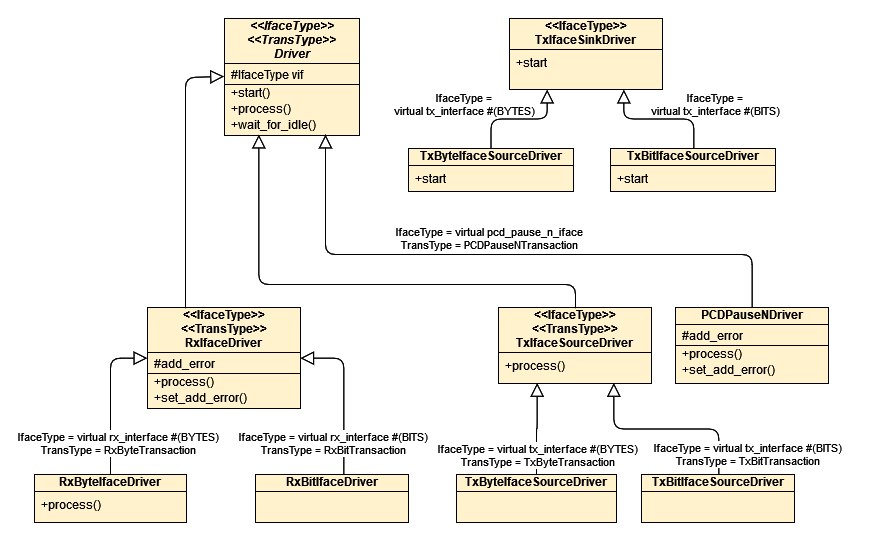
\includegraphics[width=1.0\textwidth]{./img/drivers_uml.vpd}
  \caption{Diagrama UML de clases para los controladores.}
  \label{fig:driver_uml}
\end{figure}

% Monitores
\FloatBarrier
\subsection{Monitores}

La \figref{fig:monitor_uml} muestra el diagrama UML de las clases para los monitores. La clase base es \textbf{Monitor}, es abstracta y tiene dos tipos parametrizados: \textit{IfaceType}, que es el tipo de la interfaz que monitoriza, y \textit{TransType}, que es el tipo de las transacciones que construye. El método \textbf{start()} lleva una referencia a una cola de elementos de tipo \textit{TransType} y comienza un nuevo hilo de ejecución. Ese hilo llama el método \textbf{process()}, si esa tarea devuelve una transacción válida, es empujada a la cola, para que el banco de prueba pueda verificarla, y el método \textbf{process()} es llamado de nuevo. Ese proceso se repite por siempre. En esta clase base \textbf{process()} es abstracto, las clases hijas lo sustituyen para definir cómo armar una transacción desde las señales de la interfaz.

\vfill

\begin{figure}[htb]
  \centering
  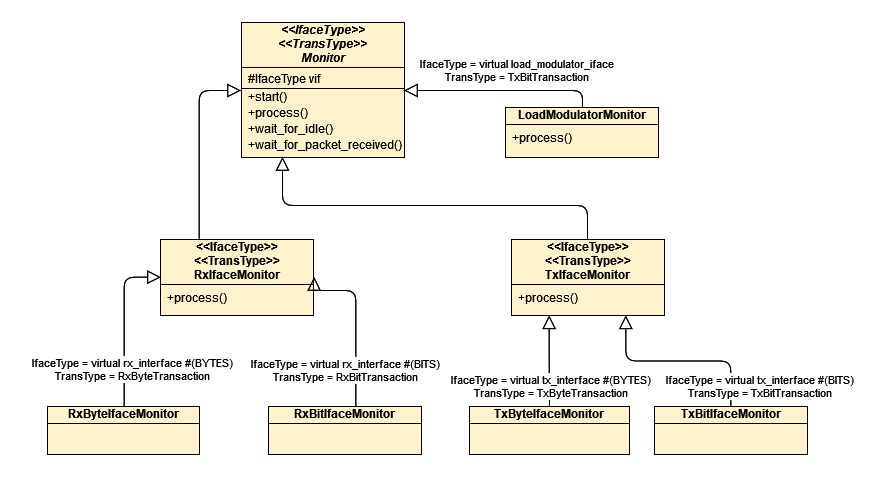
\includegraphics[width=1.0\textwidth]{./img/monitors_uml.vpd}
  \caption{Diagrama UML de clases para los monitores.}
  \label{fig:monitor_uml}
\end{figure}

Para la \textit{rx\_interface}, las clases son \textbf{RxIfaceMonitor} y sus hijas \textbf{RxByteIfaceMonitor} y \textbf{RxBitIfaceMonitor}. El método \textbf{process()} monitoriza la \textit{rx\_interface} para una de las señales: \textit{SOC}, \textit{EOC}, \textit{error} o \textit{data\_valid} tener valor ‘1’. Cuándo \textit{SOC} está en ‘1’ comienza construir una nueva transacción. Cuándo \textit{data\_valid} está en ‘1’ el bit o byte actual en la señal \textit{data} es empujado a la cola de datos en la transacción. Cuándo \textit{error} está en ‘1’ la transacción es actualizada para indicar la detección del error. Finalmente cuándo \textit{EOC} está en ‘1’ indicando el fin de la trama, la transacción es devuelta. Si detecta un error, por ejemplo un SOC dentro de una trama, o un EOC fuera de una trama, un error es indicado al usuario mediante la función de sistema \textbf{\$error()}, la transacción es abandonada, y un error es devuelto.

Los monitores para la \textit{tx\_interface} son parecidos a los monitores de recepción, salvo por el método \textit{process()}. Este método primero espera hasta que la señal \textit{data\_valid} esté en ‘1’, que indica el comienzo de una trama. Cuándo la señal \textit{req} está en ‘1’, significa que el sumidero ha leído el último dato, así el monitor agrega el bit o byte actual en la señal \textit{data} a la transacción. Cuándo \textit{data\_valid} baja a ‘0’, significa que la fuente no tiene más datos a enviar siendo el fin de la trama, y la transacción es devuelta.

Finalmente la clase \textbf{LoadModulatorMonitor} es diseñada para monitorear y decodificar la señal \textit{lm\_out} que es conectada al modulador de carga en el AFE. El método \textbf{process()} primero espera por un flanco ascendente de la señal \textit{lm\_out}, y después toma una muestra de la señal cada ciclo para 128 ciclos, lo que es la duración para enviar un bit. Si las muestras son iguales al patrón definido en la norma para envíar un ‘1’ o ‘0’ lógico, ese valor lógico es agregado a la transacción. Cuándo todas las muestras están ‘0’s indica el fin de la trama y la transacción es devuelta. Las muestras teniendo cualquier otro patrón indican un error, y el monitor llama la función de sistema \textbf{\$error()} para avisar al usuario.

% Generador y Conversores de Transacciones
\FloatBarrier
\subsection{Generador y Conversores de Transacciones}

El generador de transacciones es una clase \textbf{TransactionGenerator}, que tiene métodos para generar transacciones para todos las tramas definidas en la norma. Por tramas de recepción (PCD a PICC) las transacciones generadas son de tipo \textbf{RxByteTransactions}. Transacciones de tipo \textbf{TxByteTransactions} son generadas por tramas de transmisión (PICC a PCD). También hay métodos para generar transacciones desde una cola de bytes, y para generar transacciones aleatorias restringidas a no ser las tramas definidas en la norma. Las transacciones pueden tener CRCs agregadas automáticamente si es deseado por el usuario. Además es posible pedir que el CRC agregado sea corrompido para verificar como un módulo maneja tramas con errores de CRC.

Los conversores de transacciones son clases que facilitan la conversión de un tipo de transacción a otro. Un ejemplo del uso de un conversor de transacciones es: convirtiendo una \textbf{RxByteTransaction} generada por el generador de transacciones a una \textbf{RxBitTransaction} que el controlador \textbf{RxBitIfaceDriver} puede enviar sobre una \textit{rx\_interface} de bits. La clase base abstracta es \textbf{TransactionConverter}. Esta clase tiene dos tipos parametrizados: \textit{InputTransType} y \textit{OutputTransType} que especifican los tipos de las transacciones involucradas en la conversión. Las clases son:

\begin{itemize}
  \item \textbf{RxByteToByteTransactionConverter}: Convertir una \textbf{RxByteTransaction} a una \textbf{RxByteTransaction} (identidad).
  \item \textbf{RxByteToBitTransactionConverter}: Convertir una \textbf{RxByteTransaction} a una \textbf{RxBitTransaction}, opcionalmente agregando los bits de paridad.
  \item \textbf{RxBitToPCDPauseNTransactionConverter}: Convertir una \textbf{RxBitTransaction} a una \textbf{PCDPauseNTransaction}.
  \item \textbf{RxByteToPCDPauseNTransactionConverter}: Convertir una \textbf{RxByteTransaction} a una \textbf{PCDPauseNTransaction}, opcionalmente agregando los bits de paridad.
  \item \textbf{TxByteToByteTransactionConverter}: Convertir una \textbf{TxByteTransaction} a una \textbf{TxByteTransaction} (identidad).
  \item \textbf{TxByteToBitTransactionConverter}: convertir una \textbf{TxByteTransaction} a una \textbf{TxBitTransaction}, opcionalmente agregando los bits de paridad.
\end{itemize}

% Secuencias
\FloatBarrier
\subsection{Secuencias}

Las clases de secuencias no deberían ser confundidas con el método que el PCD usa para codificar tramas mediante pausas, estas clases son diseñadas para verificar el comportamiento de módulos que reciben tramas desde el PCD, y responden con las respuestas adecuadas. Contienen una serie de pruebas que: ponen el DUT en un estado conocido, envían una o más tramas, verifican que las respuestas son las esperadas, y que el estado del DUT cambia como se espera. Cada banco de prueba que necesita usar una secuencia debería extender una de las secuencias genéricas para proveer el funcionamiento específico para el DUT.

La clase base es \textbf{Sequence}, y contiene atributos:

\begin{itemize}
  \item \textit{rx\_trans\_gen} y \textit{tx\_trans\_gen}, los generadores de transacciones de recepción y transmisión.
  \item \textit{rx\_trans\_conv} y \textit{tx\_trans\_conv}, los conversores de transacciones para recepción y transmisión.
  \item \textit{rx\_driver}, el controlador para enviar tramas sobre la \textit{rx\_interface}.
  \item \textit{rx\_send\_queue}, una referencia a una cola conectada al \textit{rx\_driver}. Las transacciones empujadas a esa cola son enviadas por el controlador.
  \item \textit{tx\_monitor}, el monitor para monitorizar la \textit{tx\_interface}.
  \item \textit{tx\_recv\_queue}, una referencia a una cola conectada al \textit{tx\_monitor}. Tramas detectadas sobre la \textit{tx\_interface} son empujadas a esa cola.
\end{itemize}

Y estos métodos:

\begin{itemize}
  \item \textbf{send\_transaction()}: Lleva una \textbf{RxByteTransaction}, la convierte a una transacción del tipo requerido mediante el conversor de transacciones \textit{rx\_trans\_conv}, la empuja a la cola \textit{rx\_send\_queue} y espera para el controlador \textit{rx\_driver} terminar enviarla.
  \item \textbf{send\_*()}: Hay un método para cada trama definida en la norma: por ejemplo \textbf{send\_reqa()} o \textbf{send\_select()}. Generan una transacción para la trama mediante el generador de transacciones \textit{rx\_trans\_gen}, y la pasa a \textbf{send\_transaction()}.
  \item \textbf{wait\_for\_reply()}: Espera para el monitor \textit{tx\_monitor} a indicar que ha recibido una transacción, quita la transacción de la cola \textit{tx\_recv\_queue} y la devuelve. Hay una aserción para confirmar que la transacción es recibida dentro de un periodo de tiempo especificado.
  \item \textbf{verify\_no\_reply()}: Espera un periodo de tiempo especificado para confirmar que el DUT no envía una trama.
  \item \textbf{verify\_trans()}: Verifica que una transacción recibida es igual a la que es esperada.
  \item \textbf{sequence\_callback()}: Los bancos de pruebas pueden sustituir ese método para permitir actuar sobre eventos de forma específica al banco de prueba.
\end{itemize}
La clase \textbf{SpceficTargetSequence} extiende \textbf{Sequence} con la intención de verificar el comportamiento de una PICC en particular, o parte de su diseño. El UID de la PICC es conocido, permitiendo la predicción de sus acciones y respuestas. Esa clase sustituye unos de los métodos de la clase base para seguir y verificar el estado de la PICC, por ejemplo si la PICC es en estado IDLE y una REQA es enviada, la PICC debería transicionar al estado READY y enviar la respuesta ATQA. También hay unos métodos definidos que envían las tramas necesarias para inducir al DUT a transicionar a un estado especificado.

Siguiente la clase \textbf{CommsTestsSequence} extiende \textbf{SpecificTargetSequence}. Esta clase contiene una serie de pruebas para verificar el comportamiento de una PICC, o parte de su diseño. Las pruebas específicas son descritas más adelante en la sección de implementación cuándo son usados. Un ejemplo de una prueba típica es:

\begin{itemize}
  \item Transicionar al estado READY o READY* aleatoriamente.
  \item Enviar la trama SELECT con el UID de la PICC pero con CRC corrompida.
  \item Verifica que el DUT no responde.
  \item Verifica que el DUT está en estado IDLE o HLTA dependiendo si el estado original estuvo READY o READY* respectivamente.
\end{itemize}

% Otros
\FloatBarrier
\subsection{Otros}

Los controladores y monitores siendo clases no pueden utilizar señales de forma directa, tienen que usar una interfaz, por lo tanto hay dos interfaces más definidas para uso solo en verificación:

\begin{itemize}
  \item \textit{pcd\_pause\_n\_iface}: Es usada con el controlador \textbf{PCDPauseNDriver}. Contiene una señal de un bit: \textit{pause\_n}, que representa la entrada desde el detector de pausas del AFE.
  \item \textbf{load\_modulator\_iface}: Es usada con el monitor \textbf{LoadModulatorMonitor}. También consiste en una señal de un bit: \textit{lm}, que representa la salida hasta el modulador de carga del AFE.
\end{itemize}

La clase de ayuda \textbf{UID} está diseñada para ayudar con operaciones relacionadas con el UID de una PICC. Puede ser usada para guardar un UID simple, doble o triple. También puede ser usada para comparar los datos en una trama ANTICOLLISION o SELECT con el UID de la PICC, para conocer si es esperado que la PICC respondería a esa trama. La clase \textbf{FixedSizeUID} extiende \textbf{UID}, y tiene un parámetro para definir si el UID es simple, doble o triple. También tiene dos parámetros para especificar cuántos de los bits más significativos son constantes, y el valor de esos bits. Los bits menos significativos pueden ser generados aleatoriamente, considerando unas restricciones para asegurar que el UID generado es válido. Esta clase está diseñada en esta forma, porque la implementación del núcleo IP en este trabajo opera de la misma manera.

La clase \textbf{StdBlockAddress} guarda detalles sobre los campos CID y NAD de los bloques estándares definidos en la parte cuatro de la norma. Esta clase es usada para generar transacciones que representan tramas de bloques estándares.

La clase \textbf{Target} contiene información sobre una PICC, y es usada para ayudar las secuencias seguir el estado de la PICC. La información guardada consiste en: La \textbf{UID}, la \textbf{StdBlockAddress} actual, y el nivel de lazo de anticolisión actual. Además contiene métodos ayudantes para operaciones comunes, por ejemplo para decodificar si una \textbf{StdBlockAddress} es direccionada a esta PICC o no.

% Modelos Analógicos
\FloatBarrier
\subsubsection{Modelos Analógicos}

Un PCD genera una señal portadora de \SI{13.56}{\mega\hertz} y la usa para enviar información a PICCs en su campo electromagnético mediante la modulación de la amplitud de esa portadora. El detector de pausas en el AFE de la PICC detecta esas pausas y genera la salida digital \textit{pause\_n} para indicar cuándo las pausas son detectadas. La pausa detectada por el AFE es una distorsión de la pausa ideal enviada del dominio digital del PCD. Los dos flancos de la pausa son retrasados debido a las implementaciones del circuito de modulación de amplitud del PCD y del detector de pausas del AFE. También esa distorsión puede retardar los flancos descendente y ascendente por tiempos diferentes, cambiando la duración de la pausa. Además el AFE de la PICC recupera el reloj desde la portadora, y por lo tanto el reloj se detiene durante las pausas. Debido a las implementaciones del circuito de modulación de amplitud del PCD y de la recuperación del reloj del AFE, el reloj puede seguir andando por unos ciclos después de que el PCD comienza la pausa, y el reloj puede seguir detenido por unos ciclos después de que el PCD termina la pausa. Para simular este comportamiento, un modelo del PCD y del AFE fue implementado. La \figref{fig:analog_model} muestra ese modelo.

\begin{figure}[htb]
  \centering
  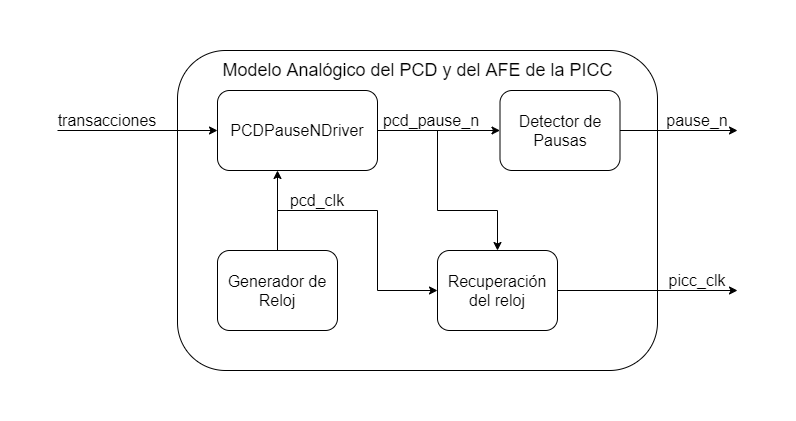
\includegraphics[width=1.0\textwidth]{./img/analogue_model}
  \caption{Modelo del PCD y del AFE de la PICC para uso en simulaciones.}
  \label{fig:analog_model}
\end{figure}

El modelo consiste en cuatro bloques:

\begin{itemize}
  \item Generador de Reloj: Genera un reloj continuo de \SI{13.56}{\mega\hertz} que es un modelo del reloj del PCD.
  \item \textbf{PCDPauseNDriver}: El controlador que envía transacciones mediante pausas. Genera una señal \textit{pcd\_pause\_n} que es la pausa ideal dentro del PCD. La duración de la pausa puede ser elegida por el usuario.
  \item Detector de Pausas: Un modelo del bloque con el mismo nombre en el AFE de la PICC. Genera una señal: \textit{pause\_n} que es una versión retrasada de la señal \textit{pcd\_pause\_n}. Los retardos del flanco ascendente y el flanco descendente pueden ser elegidos por el usuario individualmente.
  \item Recuperación del Reloj: Un modelo del bloque con el mismo nombre en el AFE de la PICC. Genera un reloj basado en lo del PCD, que se detiene durante las pausas. Los retardos entre el comienzo de una pausa y el reloj deteniéndose, y entre el fin de una pausa y el reloj comenzando de nuevo, pueden ser elegidos por el usuario individualmente. Además el usuario puede especificar que el reloj no se detiene, por lo tanto este modelo puede simular el comportamiento de un AFE dónde el reloj es continuo.
\end{itemize}

La \figref{fig:afe_sim} muestra dos simulaciones de una pausa con argumentos de timing diferentes. En el momento de escritura de esta tesis los timings por defectos son basados en simulaciones SPICE del AFE implementado por Alcalde Bessia por otro proceso de fabricación~\cite{fabricio_eamta}. Cuándo exista una implementación del AFE para el proceso de fabricación XFAB XH018 es altamente sugerido que los valores en este modelo sean actualizados para adecuarse la situación real.

\begin{figure}[htb]
  \centering
  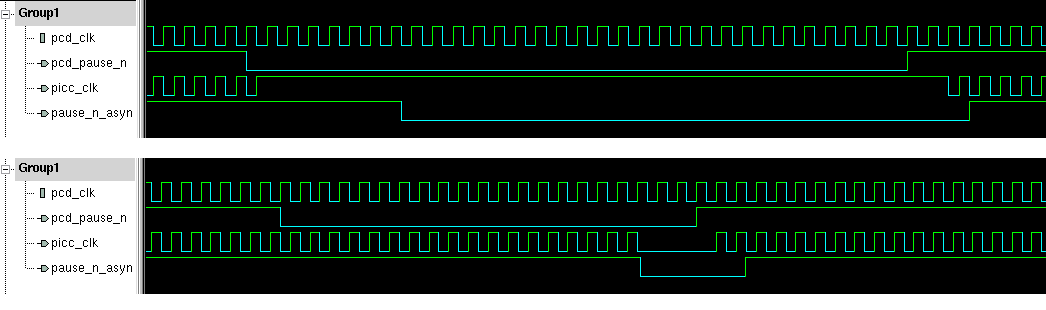
\includegraphics[width=1.0\textwidth]{./img/analogue_sim}
  \caption{Dos ejemplos con timings diferentes del modelo analógico del PCD y el AFE de la PICC.}
  \label{fig:afe_sim}
\end{figure}

% Estructura de los Bancos de Pruebas
\FloatBarrier
\subsection{Estructura de los Bancos de Pruebas}

La mayoría de los módulos en esta tesis son verificados con un banco de prueba que tiene una de las dos estructuras mostrado en la \figref{fig:tb_structures}.

Los módulos que simplemente reciben tramas, operan sobre ellas, y las reenvían, son verificados con un banco de prueba sin una secuencia (izquierda). El bloque de control genera una transacción en el formato adecuado y la pasa al controlador mediante un FIFO. El DUT la recibe por su interfaz de sumidero, la procesa, y la reenvía sobre su interfaz de fuente. El monitor detecta la trama reenviada, construye una transacción, y la pasa al bloque de control mediante otro FIFO. Finalmente el bloque de control compara esas transacciones para verificar que la trama fue modificada correctamente.

Los módulos que reciben solicitudes del PCD y envían respuestas, son verificados con un banco de prueba que incluye una secuencia (derecha). El banco de prueba define una nueva clase de secuencia que extiende una de las secuencias genéricas, y sustituye varios métodos para implementar funcionamiento específico a ese banco de prueba. Esos bancos de pruebas funcionan de una manera parecida a los bancos de prueba sin secuencias, pero las tramas enviadas son elegidas por las pruebas en la secuencia, y son generadas por el generador de transacciones. Además las respuestas enviadas por el DUT son comparadas en la secuencia con las respuestas esperadas.

\begin{figure}[htb]
  \centering
  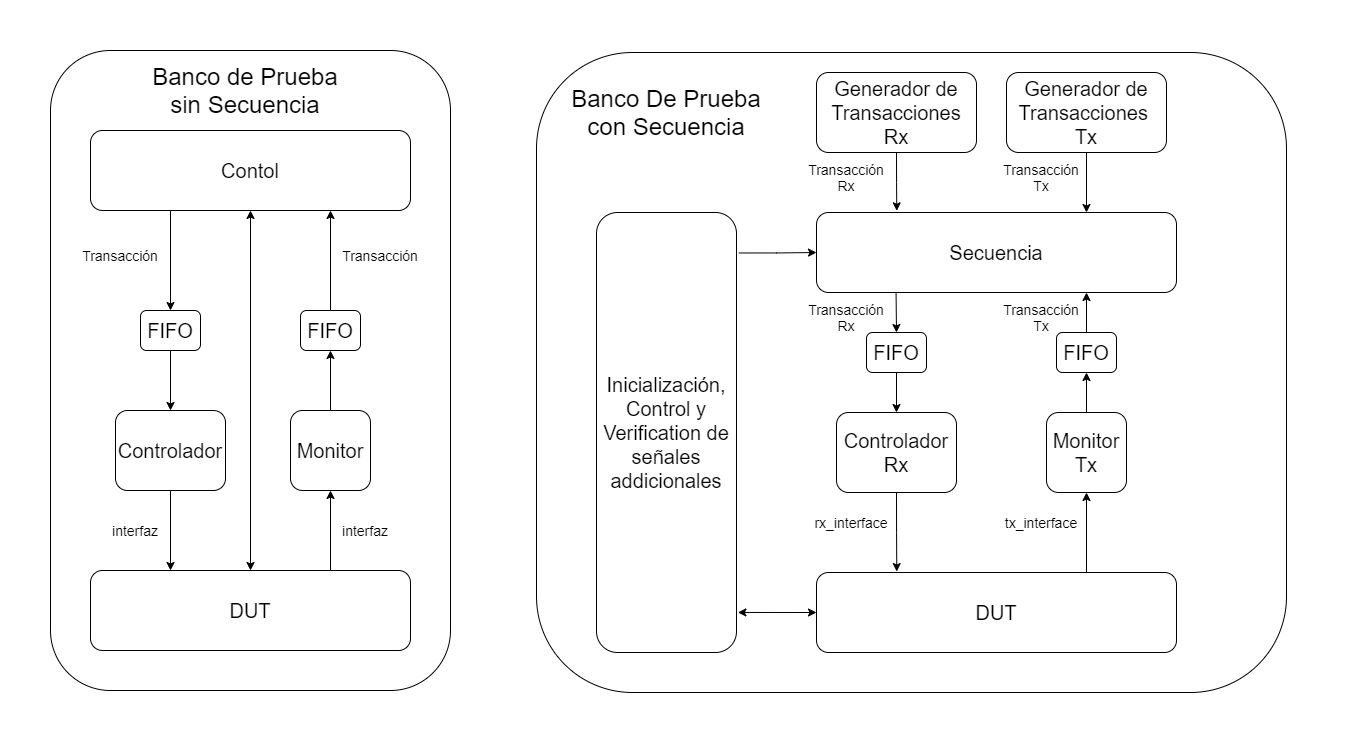
\includegraphics[width=1.0\textwidth]{./img/verification3}
  \caption{Dos estructuras comunes de los bancos de pruebas.}
  \label{fig:tb_structures}
\end{figure}

% ISO/IEC 14443A núcleo IP
% --------------------------------
\FloatBarrier
\section{ISO/IEC 14443A núcleo IP}

Está parte de la tesis está diseñada para ser una implementación digital genérica de la norma ISO/IEC 14443 para PICCs tipo A. Cuándo se combina con una AFE puede ser usado para cualquier proyecto que requiera funcionar como una PICC tipo A. La implementación  se divide en tres partes principales para las partes dos, tres, y cuatro de la norma.

% ISO/IEC 14443-2A
\FloatBarrier
\subsection{ISO/IEC 14443-2A}

Está parte de la implementación consiste en cinco módulos y sus bancos de pruebas correspondientes. Para la ruta de recepción de tramas hay un solo módulo: \textbf{sequence\_decode}, que convierte una serie de pausas a tramas de bits. La ruta de transmisión consiste en tres módulos que convierten tramas de bits a una señal apta para manejar el modulador de carga. Las módulos son:

\begin{itemize}
  \item \textbf{subcarrier}: Genera la subportadora.
  \item \textbf{bit\_encoder}: Genera la codificación manchester desde una trama de bits.
  \item \textbf{tx}: Recibe la trama a transmitir, agrega el SOC, y produce la salida al modulador de carga mediante los módulos: \textbf{subcarrier} y \textbf{bit\_encode}.
\end{itemize}

Finalmente hay un módulo: \textbf{iso14443\_2a} que es el módulo más alto de esta parte de la norma.

% subcarrier
\FloatBarrier
\subsubsection{subcarrier}

Este módulo genera la señal de la subportadora cuándo pedido. Las entradas y salidas son descritas en el \tabref{tab:ports_subcarrier}. La norma dicta que la subportadora debería tener frecuencia igual a $\nicefrac{f_c}{16}$, y que el periodo de bit debería comenzar con el estado cargado de la portadora~\cite{iso14443-2}. Esto significa que la salida \textit{subcarrier} es una onda cuadrada que comienza con valor ‘1’, y tiene un periodo de 16 ciclos del reloj.

\begin{table}[htb]
  \centering
  \tablezebra
  \begin{tabulary}{\linewidth}{l|l|L}
    \textbf{Nombre}&\textbf{Dirección}&\textbf{Descripción} \\
    \hline
    clk&Entrada&Reloj. \\
    rst\_n&Entrada&Reset activo bajo. \\
    en&Entrada&Señal de habilitación. \\
    subcarrier&Salida&Subportadora. \\
  \end{tabulary}
  \caption{Entradas y Salidas del módulo \textbf{subcarrirer}.}
  \label{tab:ports_subcarrier}
\end{table}

La implementación consiste en un contador de tres bits, cuándo el módulo no está activado el contador es detenido con valor cero, y la salida \textit{subcarrier} está ‘0’. Cuándo la señal \textit{en} sube a ‘1’, la salida \textit{subcarrier} es asignada a ‘1’ y el contador comienza a contar. Cada ocho ciclos del reloj el contador completa su cuenta, y la salida \textit{subcarrier} invierte su estado lógico.

El banco de prueba consiste en activar el DUT tres veces. La primera vez es activado por 256 ciclos (dos duraciones de bits). La segunda vez es activado por seis ciclos, para que la subportadora sea ‘1’ cuando se desactiva el DUT. Finalmente la tercera vez el módulo es activado por trece ciclos, para que la subportadora sea ‘0’ cuando se desactiva el DUT. Hay cuatro aserciones que verifican el comportamiento:

\begin{itemize}
  \item La subportadora está ‘0’ mientras el DUT está en reset.
  \item La subportadora está ‘0’ mientras el DUT está desactivado.
  \item Un ciclo después del flanco ascendente de la señal \textit{en} el subcarrier está ‘1’.
  \item Cuando el DUT está activado la subportadora tiene un periodo de 16 ciclos del reloj con un ciclo de trabajo de 50\%.
\end{itemize}

El informe de cobertura da un resultado de 100\% cobertura.

% bit_encoder
\FloatBarrier
\subsubsection{bit\_encoder}

Este módulo es un sumidero para la \textit{tx\_interface}, recibe tramas de bits y las convierte a su codificación Manchester con duración de bit de 128 ciclos del reloj. Las entradas y salidas son descritas en el \tabref{tab:ports_bit_encoder}.

\begin{table}[htb]
  \centering
  \tablezebra
  \begin{tabulary}{\linewidth}{l|l|L}
    \textbf{Nombre}&\textbf{Dirección}&\textbf{Descripción} \\
    \hline
    clk&Entrada&Reloj. \\
    rst\_n&Entrada&Reset activo bajo. \\
    en&Entrada&Señal de habilitación. \\
    in\_iface&Entrada&Sumidero de la, \textit{tx\_interface}. Las tramas a transmitir. \\
    encoded\_data&Salida&Codificación Manchester de cada bit. \\
    last\_tick&Salida&Indica el último ciclo de cada periodo de bit. \\
  \end{tabulary}
  \caption{Entradas y Salidas del módulo \textbf{bit\_encoder}.}
  \label{tab:ports_bit_encoder}
\end{table}

La implementación de este módulo consiste en un contador de siete bits para contar la duración de bit de 128 ciclos. Cuando el módulo no está activado el contador tiene valor cero, y cuando está activado cuenta repetitivamente. Al principio de cada duración de bit, eso es decir cuándo el contador tiene valor cero y el módulo está activado, la salida \textit{encoded\_data} es asignada al valor del bit actual presente en la \textit{in\_iface}. En el medio del periodo del bit, cuando el contador tiene valor 64, la salida \textit{encoded\_data} se invierte. Esto significa que para envíar el bit 0, \textit{encoded\_data} está ‘0’ por 64 ciclos y después ‘1’ por 64 ciclos más. La señal \textit{tx\_interface.req} está pulsada por un ciclo del reloj en el medio del periodo de bit, para pedir que la fuente prepare el siguiente bit. Finalmente la salida \textit{last\_tick} está pulsada cuándo el contador tiene valor 127, esta salida es usada para determinar cuándo desactivar este módulo después del último bit de la trama.

El banco de prueba tiene un \textbf{TxBitIfaceSourceDriver} para envíar tramas al DUT. No utiliza un monitor, ya que es el único módulo que genera una salida en este formato. Antes de envíar cada trama, la transacción es convertida a una cola que consiste en los valores esperados por cada ciclo de la trama. Una aserción verifica que la salida \textit{encoded\_data} del DUT corresponde con esa cola. Las pruebas consisten en:

\begin{itemize}
  \item Enviar dos transacciones de un solo bit cada una, con valores ‘0’ y ‘1’.
  \item Enviar dos transacciones de dos bit cada una, con valores “00” y “10”.
  \item Enviar mil transacciones de data y tamaño aleatorios.
\end{itemize}

Las aserciones son:

\begin{itemize}
  \item Cuándo el DUT está en reset o no está activado, las salidas: \textit{in\_iface.req} y \textit{last\_tick} están ‘0’s.
  \item La salida \textit{last\_tick} solo está ‘1’ para un ciclo del reloj a la vez.
  \item Mientras el DUT está activado, las salidas \textit{in\_iface.req} y \textit{last\_tick} pulsan por un ciclo del reloj, cada 128 ciclos.
  \item Después del flanco ascendente de la entrada \textit{en}, la salida \textit{last\_tick} está ‘0’ por 127 ciclos del reloj y ‘1’ en el siguiente ciclo.
\end{itemize}

El informe de cobertura da un resultado de 100\% por el DUT.

% tx
\FloatBarrier
\subsubsection{tx}

El módulo \textbf{tx} instancia los módulos: \textbf{subcarrier} y \textbf{bit\_encoder}, e incluye una máquina de estados sencilla que: agrega el SOC a las tramas, activa los submódulos, y manejar la señal \textit{tx\_interface.req} para pedir que la fuente prepare el siguiente bit. Finalmente la señal \textit{lm\_out} es el AND lógico de la subportadora y la señal \textit{encoded\_data}, esta salida es registrada para prevenir glitches llegando al modulador de carga. Las entradas y salidas son descritas en el \tabref{tab:ports_tx}.

\begin{table}[htb]
  \centering
  \tablezebra
  \begin{tabulary}{\linewidth}{l|l|L}
    \textbf{Nombre}&\textbf{Dirección}&\textbf{Descripción} \\
    \hline
    clk&Entrada&Reloj. \\
    rst\_n&Entrada&Reset activo bajo. \\
    in\_iface&Entrada&Sumidero de la \textit{tx\_interface}. \\
    lm\_out&Salida&Señal hacia el modulador de carga. \\
  \end{tabulary}
  \caption{Entradas y Salidas del módulo \textbf{tx}.}
  \label{tab:ports_tx}
\end{table}


El banco de prueba tiene un controlador \textbf{TxBitIfaceSourceDriver} y un monitor \textbf{LoadModulatorMonitor}. Las pruebas son:

\begin{itemize}
  \item El SOC es agregado correctamente. Esto es hecho en el monitor, que verifica que todas las tramas comienzan con un SOC.
  \item La salida \textit{lm\_out} está en ‘0’ cuándo la fuente no está enviando una trama.
  \item Tramas son enviadas correctamente. Cien transacciones aleatorias son enviadas y las transacciones detectadas por el monitor son comparadas a las enviadas dentro de una aserción.
\end{itemize}

El informe de cobertura da un resultado de 93\% por el DUT. Las partes que faltan cobertura no son relevantes, por ejemplo no hay una transición desde el estado State\_SOC al estado State\_IDLE, ya que no está permitido transmitir una trama SOC aislada.

% sequence_decode
\FloatBarrier
\subsubsection{sequence\_decode}
\label{sec:sequence_decode}

El módulo \textbf{sequence\_decode} convierte series de pausas a tramas de bits, y las envía al siguiente módulo mediante una fuente de la \textit{rx\_interface}. La norma ISO/IEC 14443-2~\cite{iso14443-2} especifica que la duración de bit por recepción es 128 ciclos de la portadora. La existencia de una pausa dentro de una duración de bit y su ubicación determina qué tipo de secuencia es: X, Y o Z. Una pausa al principio de la duración de bit es una secuencia Z, una pausa en el medio de la duración de bit es una secuencia X, y una duración de bit sin pausas es una secuencia Y.  La \figref{fig:sequences} muestra estas secuencias. Cada trama comienza con una secuencia Z (SOC). Un ‘1’ es transmitido con una secuencia X. La secuencia usada para transmitir un ‘0’ depende en la última secuencia. Una secuencia Y es usada cuando la última secuencia fue una X, y una secuencia Z es usada en otros casos. Cada trama termina con un EOC, que es transmitido con un ‘0’ lógico seguido por la secuencia Y. Finalmente una secuencia X seguida por una secuencia Z no es permitido y debería estar contado como un error.

En teoría el proceso de convertir una serie de pausas a secuencias es: contar el número de ciclos del reloj en cada duración de bit para determinar dónde comienza la pausa. En la práctica es más complicado debido a que el reloj puede detenerse durante las pausas. Además el tiempo que el reloj está detenido depende de la implementación del bloque de la recuperación del reloj del AFE, y las propiedades del PCD. Debido a que este núcleo IP está diseñado para ser genérico, tiene que funcionar con diferentes AFEs y diferentes PCDs, por lo tanto este módulo fue implementado para funcionar con un amplio rango de comportamientos de relojes. La estrategia propuesta para el módulo \textbf{sequence\_decode} consiste en contar ciclos de clock entre flancos ascendentes de la señal \textit{pause\_n}. Luego a partir del valor de la cuenta se infiere la secuencia recibida. A continuación se analizan las condiciones para aplicar este método de decodificación.

La \figref{fig:rx_timings_tz2z} muestra dos secuencias Z consecutivas. \textit{PCD CLK} y \textit{PICC CLK} son los relojes en el PCD y la PICC respectivamente, \textit{pcd\_pause\_n} es la pausa digital que el PCD transmite, \textit{picc\_pause\_n} es la pausa detectada en el AFE, \textit{PICC CLK ACTIVE} indica cuándo el reloj de la PICC está activo. El tiempo entre los dos flancos ascendentes de las pausas medido en ciclos del reloj del PCD es $T_b = 128$. Si el reloj de la PICC se detiene por $T_{nc}$ ciclos durante las pausas, la PICC mediría $T_{z2z} = T_b - T_{nc}$ ciclos entre los flancos ascendentes de las pausas.

\begin{figure}[htb]
  \centering
  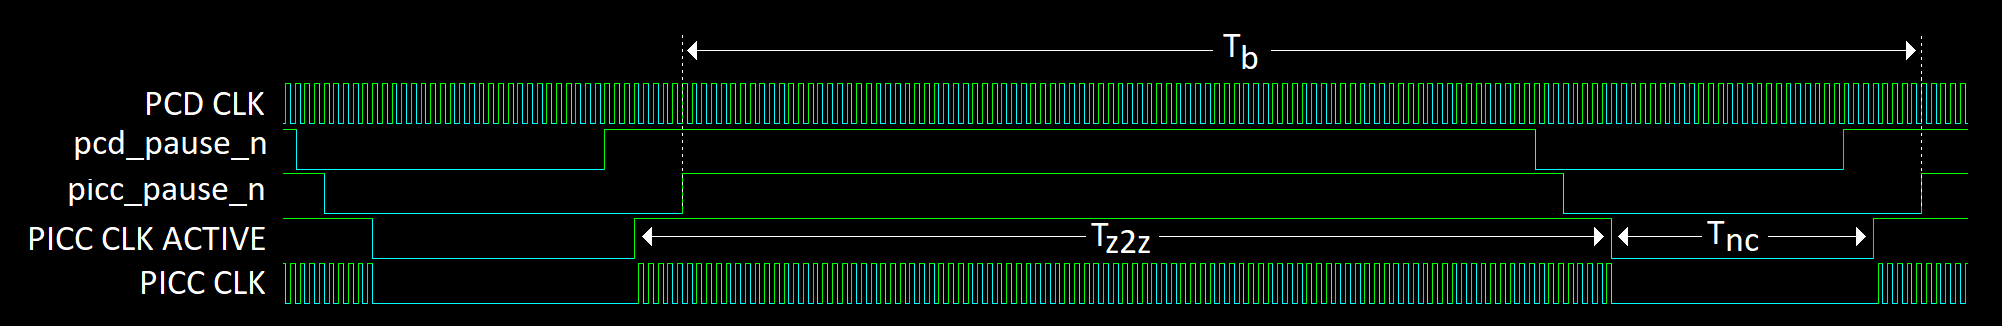
\includegraphics[width=1.0\textwidth]{./img/rx_timings_tz2z}
  \caption{Diagrama de timing de dos pausas y el comportamiento del reloj de la PICC.}
  \label{fig:rx_timings_tz2z}
\end{figure}

La \figref{fig:rx_timings} muestra el número de ciclos entre dos pausas para todas las combinaciones de secuencias posibles. Usa la misma convención de la \figref{fig:rx_timings_tz2z}, $T_{z2x}$ por ejemplo representa la cantidad de ciclos que la PICC mide entre los flancos ascendentes de las pausas cuándo el PCD transmite una secuencia Z seguida por una secuencia X. Esta convención sigue válida aun cuándo el AFE produce un reloj continuo, y por lo tanto $T_{nc}$ = 0.

\begin{figure}[htb]
  \centering
  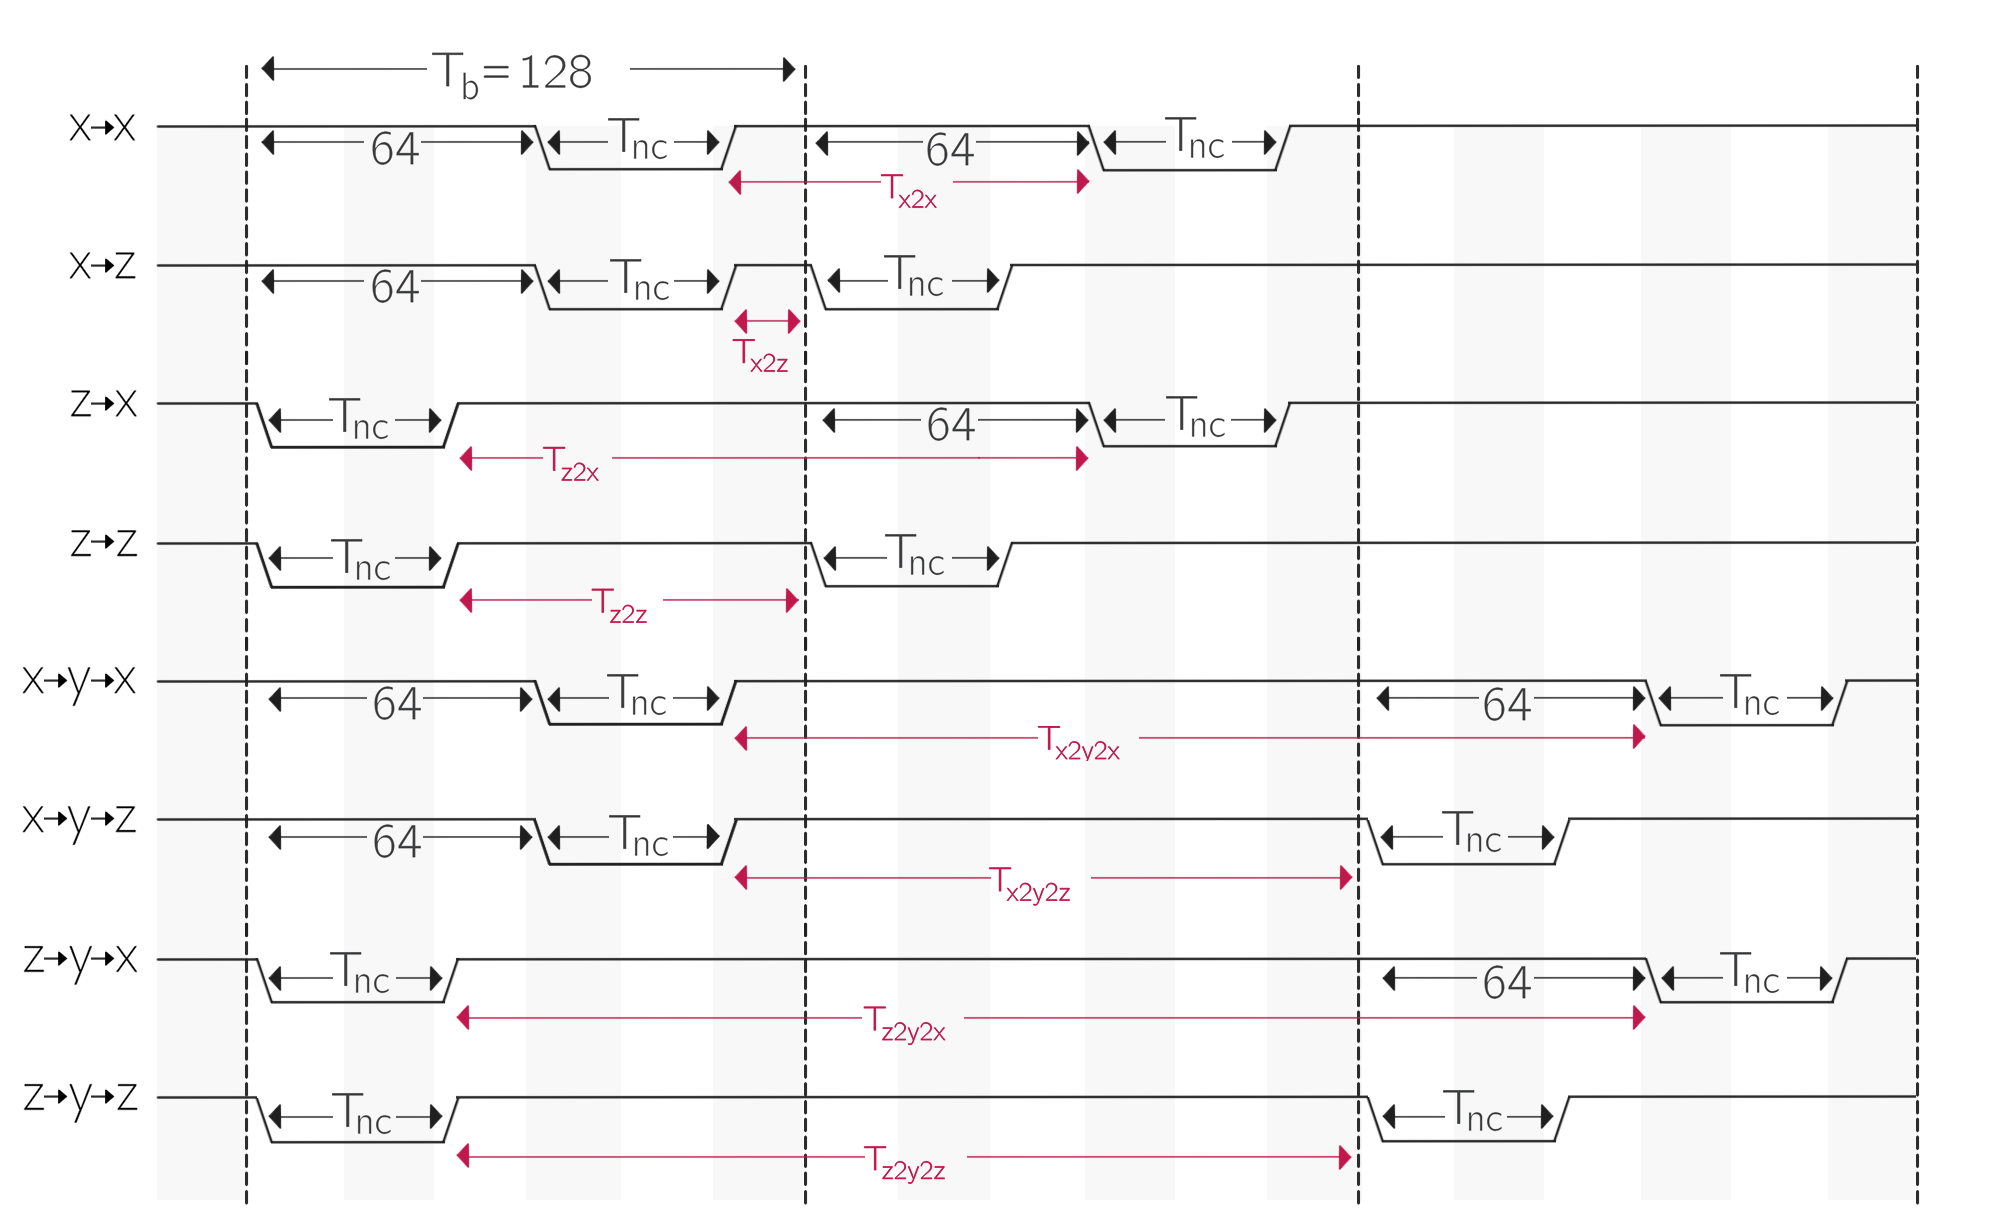
\includegraphics[width=1.0\textwidth]{./img/rx_timings}
  \caption{Números de ciclos posibles entre dos pausas.}
  \label{fig:rx_timings}
\end{figure}

Se define $T_{nc\_min}$ y $T_{nc\_max}$ como el número de ciclos mínimos y máximos que el reloj puede estar detenido para que las secuencias puedan ser decodificadas correctamente. Este análisis es necesario para considerar variaciones en el comportamiento de los PCDs y los AFEs. Considerando las combinación de secuencias: Z~$\rightarrow$~Z, y Z~$\rightarrow$~X y observando la \figref{fig:rx_timings}, se puede calcular:

\begin{align*}
    T_{z2z\_max} &= 128 - T_{nc\_min} \\
    T_{z2x\_min} &= 192 - T_{nc\_max} \\
\end{align*}

Conociendo que $T_{z2x\_min} > T_{z2z\_max}$, para que se pueda distinguir entre una Z~$\rightarrow$~X y una Z~$\rightarrow$~Z, se puede derivar:

\begin{align*}
    192 - T_{nc\_max} &> 128 - T_{nc\_min} \\
    T_{nc\_max} &< T_{nc\_min} + 64 \\
\end{align*}

Para soportar AFEs que usan un PLL para proveer un reloj continuo, debería aceptarse $T_{nc\_min}$ igual a 0. Además es posible que haya jitter en la detección de los flancos ascendentes de las las pausas en el AFE. Ese jitter puede causar que una PICC cuente un número de ciclos ligeramente diferente entre dos secuencias cada vez que ocurren. Ese comportamiento es igual a si el jitter fue en el número de ciclos que el reloj está detenido. En esta implementación es requerido que ese jitter es a lo máximo tres ciclos, por lo tanto se usa un $T_{nc\_min} = -3$, lo que da un $T_{nc\_max} < 61$.

Considerando el caso de una secuencia X seguido por una secuencia Y se requiere que: $T_{x2y\_min} > T_{x2x\_max}$, es decir que después de una secuencia X, el momento que este módulo emite una secuencia Y tiene que ser después del último momento que puede llegar una pausa que indicaría otra secuencia X. Por lo tanto:

\begin{align*}
    T_{x2y\_min} &> 128 - T_{nc\_min} \\
    T_{x2y\_min} &> 131 \\
\end{align*}

Eligiendo $T_{x2y\_min} = 132$, significa que si no hay una pausa detectada por más de 131 ciclos después de una secuencia X, se asume el arribo de una secuencia Y. Finalmente considerando el serie de secuencias: X~$\rightarrow$~Y~$\rightarrow$~Z:

\begin{align*}
    T_{x2y2z\_min} &= 192 - T_{nc\_max} \\
               &= T_{x2y\_min} + T_{y2z\_min} \\
               &= 132 + T_{y2z\_min} \\
    \\
    192 - T_{nc\_max} &= 132 + T_{y2z\_min} \\
    T_{y2z\_min} &= 60 - T_{nc\_max} \\
\end{align*}

Una $T_{y2z\_min} = 0$, implica que la secuencia Y puede ser detectada en el mismo ciclo de un flanco ascendente de una pausa por una secuencia Z. Para simplificar el diseño esto no se permite, así:

\begin{align*}
    T_{y2z\_min} &> 0 \\
    60 - T_{nc\_max} &> 0 \\
    T_{nc\_max} &< 60 \\
\end{align*}

En resumen es posible diseñar un sistema que decodifica una serie de pausas a secuencias, siempre que el AFE pueda garantizar que el reloj nunca se detiene por más de 59 ciclos. Para soportar hasta $\pm 3$ ciclos de jitter en la detección de las pausas como especificado arriba es recomendado que el reloj no se detenga por más de 56 ciclos. El mismo diseño va a funcionar con un AFE que produce un reloj continuo. Estos requisitos por el AFE son razonables, debido a que la duración de pausa máxima determinada con la \figref{fig:pause} y el \tabref{tab:pause_values} es 56,5 ciclos del reloj, medido entre los puntos 1 y 2, dónde él amplitud de la portadora es a 90\% de su original.

Usando $T_{nc\_min} = -3$, y $T_{nc\_max} = 59$, es posible diseñar un sistema que decodifica pausas a secuencias, dependiendo de la última secuencia detectada y el número de ciclos contados entre los flancos ascendentes de las pausas. La decodificación usada es mostrada en el \tabref{tab:sequence_decode_timings}. Valores fuera de estos rangos son considerados errores.

\begin{table}[htb]
  \centering
  \begin{tabular}{c|r|r|c}
    \rowcolor{lightgray!35}
    \textbf{Última Secuencia} & \textbf{Mín Ciclos} & \textbf{Máx Ciclos} & \textbf{Proxima Secuencia} \\
    \hline
                        & 69             & 131   & X \\
    \multirow{-2}{*}{X} & 132 (timeout)  & -     & Y \\
    \rowcolor{lightgray!35}
                        & 69             & 131   & Z \\
    \rowcolor{lightgray!35}
                        & 132            & 195   & X \\
    \rowcolor{lightgray!35}
    \multirow{-3}{*}{Z} & 196 (timeout)  & -     & Y \\
                        & 1              & 64    & Z \\
                        & 65             & 127   & X \\
    \multirow{-3}{*}{Y} & 128 (timeout)  & -     & Y \\
  \end{tabular}
  \caption{Decodificación de pausas basado en la última secuencia y el tiempo entre pausas.}
  \label{tab:sequence_decode_timings}
\end{table}

El \tabref{tab:ports_sequence_decode} muestra las entradas y salidas de este módulo. La implementación consiste en dos partes. La primera parte determina la secuencia desde las pausas detectadas. Comienza en un estado inactivo, cuándo detecta la primera pausa emite una secuencia Z (SOC). Después emite secuencias cuándo pausas están detectadas o cuándo timeouts ocurren usando el método descrito arriba. Después de detectar dos secuencias Y consecutivas, eso es dos duraciones de bits sin pausas, se vuelve al estado inactivo, y espera por la próxima trama. En el caso de detectar un error, no emite más secuencias y después de haber detectado tres duraciones de bits sin pausas vuelve al estado inactivo. La segunda parte de este módulo decodifica las secuencias a una trama de bits y lo envía sobre la \textit{out\_iface} para el posterior procesamiento en otros módulos.

\begin{table}[htb]
  \centering
  \tablezebra
  \begin{tabulary}{\linewidth}{l|l|L}
    \textbf{Nombre}&\textbf{Dirección}&\textbf{Descripción} \\
    \hline
    clk&Entrada&Reloj. \\
    rst\_n&Entrada&Reset activo bajo. \\
    pause\_n\_synchronised &Entrada&Pausa, activa baja, sincronizada.\\
    out\_iface&Salida&Fuente de la \textit{rx\_interface}.\\
  \end{tabulary}
  \caption{Entradas y Salidas del módulo \textbf{sequence\_decode}.}
  \label{tab:ports_sequence_decode}
\end{table}

Para verificar este módulo el banco de prueba envía varias transacciones mediante el controlador \textbf{PCDPauseNDriver} en el modelo del AFE, que maneja la entrada del DUT \textit{pause\_n\_synchronised}. El monitor \textbf{RxBitIfaceMonitor}, monitoriza la salida \textit{out\_iface} y emite transacciones por las tramas detectadas. Esas transacciones son comparadas con las enviadas para verificar que el DUT decodifica correctamente las pausas. Las transacciones enviadas son:

\begin{itemize}
  \item La transacción ZZXXYZXYXYY, y la transacción ZXYZY. Estas dos transacciones verifican todas las filas en el \tabref{tab:sequence_decode_timings}.
  \item Cincuenta transacciones aleatorias sin errores.
  \item La transacción: ZXZZXYXYY para verificar que la transición Z~$\rightarrow$~X es detectada como un error, y que secuencias después del error son ignoradas.
\end{itemize}

Estas pruebas son repetidas varias veces con diferentes timings configurados en el modelo del AFE. Los parámetros de timings son:

\begin{itemize}
  \item La duración de la pausa.
  \item Si el reloj se detiene durante las pausas o no.
  \item El retardo entre el principio de una pausa del PCD y el reloj deteniéndose.
  \item El retardo entre el final de una pausa del PCD y el reloj activándose de nuevo.
  \item El retardo entre el principio de una pausa del PCD y el AFE detectándola.
  \item El retardo entre el final de una pausa del PCD y el AFE detectándola.
\end{itemize}

Para asegurar que un amplio rango de las condiciones son verificadas estos tiempos son elegidos aleatoriamente con restricciones sobre cuántos flancos el reloj de la PICC pueden faltar comparado al reloj del PCD. El código que elige esos valores toma un argumento \textit{missing\_edges} que define el número de flancos que faltan al reloj. Este argumento es usado con la sintaxis de SystemVerilog “std::randomize() with \{\}” que permite especificar una lista de variables a randomizar y una lista de condiciones que los resultados deben cumplir. Antes fue especificado que el DUT funciona si el reloj se detiene entre 0 ciclos y 59 ciclos. Esos valores corresponden con un \textit{missing\_edges} entre 0 y 118. Las pruebas son repetidos cien veces para cada uno de \textit{missing\_edges} igual a  0 a 3 y 115 a 118, y después mil veces con \textit{missing\_edges} elegido aleatoriamente entre 4 y 114.

El informe de cobertura da un resultado de 95\% por el DUT. Los tres sitios que faltan cobertura son condiciones imposibles de ocurrir, por ejemplo emitiendo una secuencia Z después de una secuencia X. La norma define una X~$\rightarrow$~Z como un error, por lo tanto cuando el DUT detecta la Z emite un error mediante \textit{out\_iface.error}, en vez de tratarla como una secuencia Z normal.

% iso14443_2a
\FloatBarrier
\subsubsection{iso14443\_2a}

Este módulo simplemente instancia los módulos: \textbf{tx} y \textbf{sequence\_decode} como se muestra la \figref{fig:iso14443_2a}. Las entradas y salidas son descritas en el \tabref{tab:ports_iso14443_2a}.

\begin{table}[htb]
  \centering
  \tablezebra
  \begin{tabulary}{\linewidth}{l|l|L}
    \textbf{Nombre}&\textbf{Dirección}&\textbf{Descripción} \\
    \hline
    clk&Entrada&Reloj. \\
    rst\_n&Entrada&Reset activo bajo. \\
    pause\_n\_synchronised &Entrada&Pausa, activa baja, sincronizada. \\
    rx\_iface&Salida&Fuente de la \textit{rx\_interface}. \\
    tx\_iface&Entrada&Sumidero de la \textit{tx\_interface}. \\
    lm\_out&Salida&Señal hacia el modulador de carga. \\
  \end{tabulary}
  \caption{Entradas y Salidas del módulo \textbf{iso14443\_2a}.}
  \label{tab:ports_iso14443_2a}
\end{table}

\begin{figure}[htb]
  \centering
  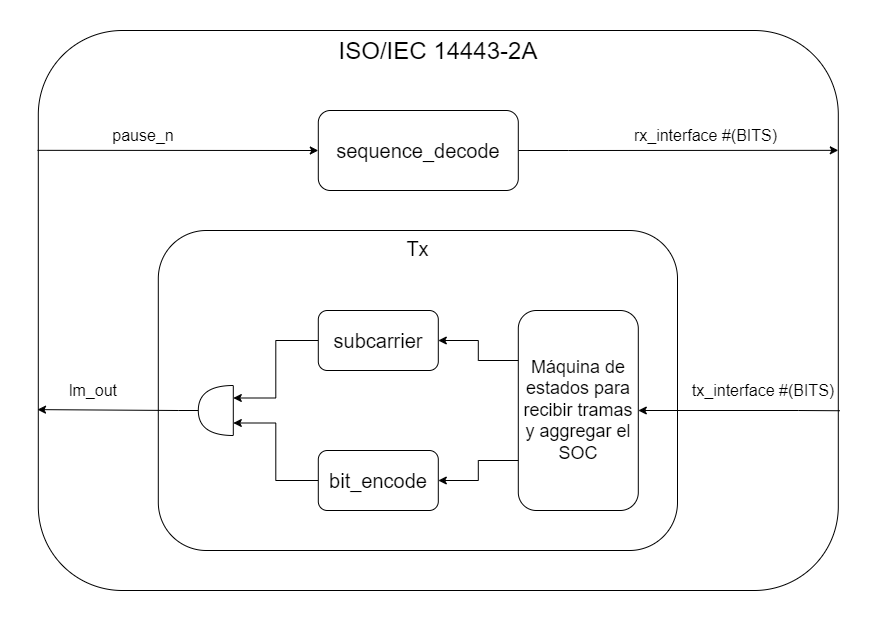
\includegraphics[width=0.8\textwidth]{./img/iso14443_2a.drawio}
  \caption{Diagrama en bloque del módulo \textbf{iso14443\_2a}.}
  \label{fig:iso14443_2a}
\end{figure}

El banco de prueba funciona de forma loopback, genera mil transacciones aleatoriamente, que son transmitidos mediante el controlador \textbf{PCDPauseNDriver} en el modelo del AFE. El monitor \textbf{RxBitIfaceMonitor} recibe las tramas procesadas por el DUT sobre la \textit{rx\_iface}. Cada transacción recibida por el monitor es convertida a una \textbf{TxBitTransaction} y es reenviado sobre la \textit{tx\_iface} con un controlador \textbf{TxBitIfaceSourceDriver}. Finalmente un monitor \textbf{LoadModulatorMonitor} detecta las tramas transmitidas por el DUT sobre su salida \textit{lm\_out}. Cada transacción recibida por ese monitor es comparada con las transacciones enviadas en una aserción. La \figref{fig:iso14443_2a_tb} muestra un diagrama en bloques del banco de prueba.

\begin{figure}[htb]
  \centering
  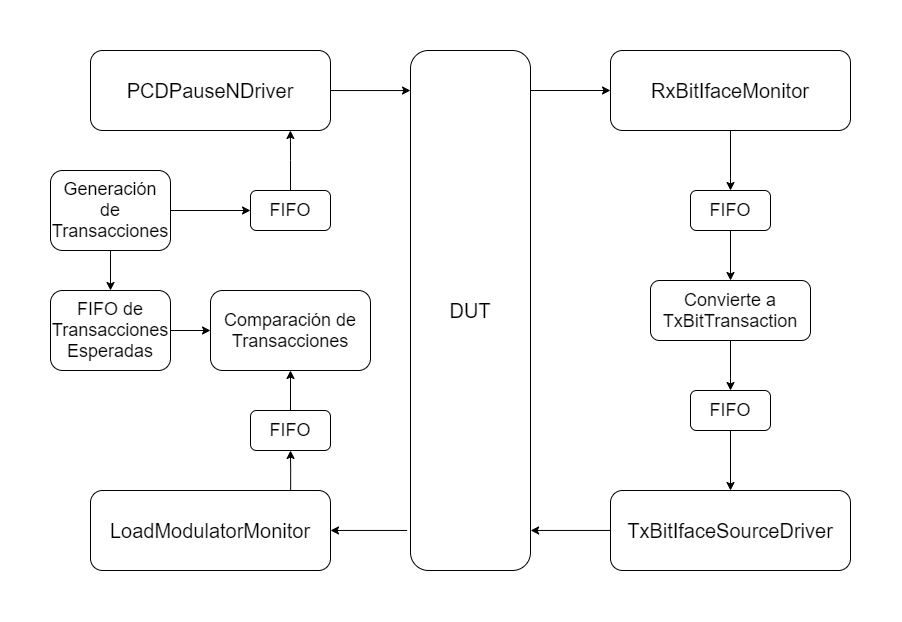
\includegraphics[width=0.9\textwidth]{./img/iso14443_2a_tb.drawio}
  \caption{Diagrama en bloques del banco de prueba para el módulo \textbf{iso14443\_2a}}
  \label{fig:iso14443_2a_tb}
\end{figure}

Debido a que este módulo solo consiste en la instanciación de dos módulos, la única métrica de cobertura generada por el DUT, no incluyendo los submódulos auxiliares, es de cambio de estado de las señales y puertos (toggle), que tiene 100\% cobertura.

% ISO/IEC 14443-3A
\FloatBarrier
\subsection{ISO/IEC 14443-3A}

Esta parte de la implementación consiste en once módulos y sus bancos de pruebas correspondientes.

\begin{itemize}
  \item \textbf{frame\_decode}: Verifica y quita los bits de paridad de tramas recibidas desde el PCD.
  \item \textbf{desreialiser}: Convierte una trama de bits a una trama de bytes. Usado en la ruta de recepción.
  \item \textbf{FDT}: Genera una señal para activar la transmisión de una respuesta, para que se cumpla con el FDT definido en la norma.
  \item \textbf{CRC\_A}: Calcula el CRC16 de una serie de bits.
  \item \textbf{crc\_control}: Verifica el CRC16 de tramas recibidas, y genera el CRC16 de tramas a transmitir.
  \item \textbf{serialiser}: Convierte una trama de bytes a una trama de bits. Usado en la ruta de transmisión.
  \item \textbf{frame\_encode}: Comienza la transmisión de una trama al PCD cuándo recibe la señal de habilitación del módulo FDT, y agrega los bits de paridad y el CRC16 a la trama.
  \item \textbf{framing}: Instancia los módulos de arriba.
  \item \textbf{initialisation}: Recibe tramas de inicialización y anticolisión desde el PCD, actúa sobre ellas, y responde con las respuestas adecuadas.
  \item \textbf{routing}: Rutea tramas recibidas desde el PCD al módulo apto para procesarlas, y rutea las respuestas desde ese módulo para transmitir al PCD. El ruteo es controlado basado en el estado actual de la PICC.
  \item \textbf{iso14443\_3a}: El módulo más alto para esta parte de la norma, instancia los módulos: \textbf{framing}, \textbf{initialisation} y \textbf{routing}.
\end{itemize}

% frame_decode
\FloatBarrier
\subsubsection{frame\_decode}

Este módulo tiene un sumidero de la \textit{rx\_interface} que está conectado a la fuente del módulo \textbf{iso14443\_2a}, y una fuente, también de la \textit{rx\_interface} que está conectado al próximo módulo. Las Tramas son recibidas en una serie de bits, después de cada 8 bits hay un bit de paridad. Esos bits de paridad son verificados y quitados antes de reenviar la trama por la fuente. Las entradas y salidas son descritas en el \tabref{tab:ports_frame_decode}.

\begin{table}[htb]
  \centering
  \tablezebra
  \begin{tabulary}{\linewidth}{l|l|L}
    % row colouring reverses here for some reason
    % This fixes it, but putting this in "non-broken"
    % tables breaks them
    \setcounter{rownum}{0}
    \textbf{Nombre}&\textbf{Dirección}&\textbf{Descripción} \\
    \hline
    clk&Entrada&Reloj. \\
    rst\_n&Entrada&Reset activo bajo. \\
    in\_iface&Entrada&Sumidero de la \textit{rx\_interface}. \\
    out\_iface&Salida&Fuente de la \textit{rx\_interface}. \\
    last\_bit&Salida&Último bit recibido. \\
  \end{tabulary}
  \caption{Entradas y Salidas del módulo \textbf{frame\_decode}.}
  \label{tab:ports_frame_decode}
\end{table}

El tipo de paridad definido por la norma es impar, eso es a decir que el número de unos en el byte más el bit de paridad debería ser impar. Por ejemplo el byte: 8’b0101\_1100, tiene cuatro ‘1’s, cuatro es par, así el bit de paridad debe ser ‘1’, para que el total de los ‘1’s sea impar.

Los bits de paridad son verificados y quitados mediante el siguiente proceso. Al principio de cada trama, un indicador \textit{expected\_parity} es inicializado a ‘1’. Después cuándo cada uno de los primeros ochos bits son recibidos, son reenviados, y ese indicador es actualizado con el resultado de: \textit{expecetd\_parity} XOR \textit{in\_iface.data}. Ese cálculo invierte el valor de \textit{expected\_parity} cada vez que un ‘1’ es recibido. El noveno bit es el bit de paridad, así es comparado con \textit{expected\_parity} para verificar que es correcto. Este proceso se repite hasta el fin de la trama, o hasta un error es detectado.

Hay tres errores que pueden ser detectados en este módulo: Un error indicado en la \textit{in\_iface}, un error en un bit de paridad, y una trama que le falta su último bit de paridad. Para soportar tramas cortas y de anticolisiones que pueden terminar con un byte parcial sin un bit de paridad, ese último error solo es emitido si una trama termina con un byte entero.

Finalmente la salida \textit{last\_bit} indica el valor del último bit recibido, incluyendo bits de paridad. Esta señal es usada en el módulo \textbf{FDT} para determinar cuándo comenzar a enviar la respuesta, debido a que el FDT usado depende en el valor de ese último bit.

El banco de prueba para este módulo consiste en un controlador \textbf{RxBitIfaceDriver} y un monitor \textbf{RxBitIfaceMonitor}. Por cada prueba una transacción es generada aleatoriamente, los bits de paridad son agregados, la transación es enviada por el controlador, el resultado es recibido por el monitor y es comparado con la transacción enviada. Las pruebas son:

\begin{itemize}
  \item Enviar una transacción de 8 bits más el bit de paridad correcto.
  \item Enviar una transacción de 8 bits más el bit de paridad equivocado.
  \item Enviar una transacción de 8 bits que falta el bit de paridad.
  \item Enviar mil transacciones de 8 bits cada uno, con un error enviado por el controlador.
  \item Enviar ocho transacciones con cero a siete bits en orden.
  \item Envíar mil transacciones cada uno con un número de bits aleatorio entre uno y ochenta, más los bits de paridad correctos.
  \item Envíar mil transacciones cada uno con un número de bits aleatorio entre ocho y ochenta, con un bit de paridad equivocado y los demás correctos.
  \item Enviar mil transacciones con un número de bytes entero entre 1 y diez, más los bits de paridad por cada byte menos el último.
\end{itemize}

Hay dos aserciones concurrentes para verificar que la señal \textit{last\_bit} es correcta. La primera confirma que la señal corresponde con el último bit enviado. La segunda verifica que esa señal no cambia entre tramas. El informe de cobertura da el DUT un resultado de 100\%.

% deserialiser
\FloatBarrier
\subsubsection{deserialiser}

Este módulo recibe tramas de bits por un sumidero de la \textit{rx\_interface} desde el módulo \textbf{frame\_decode}. Esas tramas son convertidas a tramas de bytes y reenviadas por una fuente de la \textit{rx\_interface}. La norma define que el bit menos significativo en cada byte es transmitido primero~\cite{iso14443-3}. Las entradas y salidas son descritas en el \tabref{tab:ports_deserialiser}.

\begin{table}[htb]
  \centering
  \tablezebra
  \begin{tabulary}{\linewidth}{l|l|L}
    \textbf{Nombre}&\textbf{Dirección}&\textbf{Descripción} \\
    \hline
    clk&Entrada&Reloj. \\
    rst\_n&Entrada&Reset activo bajo. \\
    in\_iface&Entrada&Sumidero de la \textit{rx\_interface}. \\
    out\_iface&Salida&Fuente de la \textit{rx\_interface}. \\
  \end{tabulary}
  \caption{Entradas y Salidas del módulo \textbf{deserialiser}.}
  \label{tab:ports_deserialiser}
\end{table}

El banco de prueba para este módulo consiste en un controlador \textbf{RxBitIfaceDriver} y un monitor \textbf{RxByteIfaceMonitor}. Por cada prueba una transacción es generada aleatoriamente, es enviada por el controlador, el resultado es recibido por el monitor y es comparado con la transacción enviada. Las pruebas son:

\begin{itemize}
  \item Enviar 17 transacciones con número de bits entre cero y 16 en orden.
  \item Enviar mil transacciones con número de bits elegido aleatoriamente entre cero y ochenta.
  \item Enviar mil transacciones con errores insertados por el controlador.
\end{itemize}

El informe de cobertura da un resultado de 100\% por el DUT.

% FDT
\FloatBarrier
\subsubsection{FDT}
\label{sec:fdt}

La norma define el FDT (Frame Delay Time) como el tiempo entre la última pausa transmitida por el PCD y el primer flanco de modulación de la respuesta enviada por la PICC~\cite{iso14443-3}. El valor del FDT requerido depende en el último bit enviado por el PCD.

\begin{tabular}{r | l}
    \textbf{Último} Bit & \textbf{FDT (en ciclos del reloj)} \\
    \hline
    '0' & $128 \cdot n + 20$ \\
    '1' & $128 \cdot n + 84$ \\
\end{tabular}

El valor de ‘n’ depende del tipo de trama enviada. Las tramas de inicialización: REQA, WUPA, ANTICOLLISION y SELECT requieren un $n = 9$, dando FDTs de 1172 ciclos y 1236 ciclos. Cualquier otra trama requiere un $n \ge 9$. Sin embargo para simplicidad esta implementación siempre usa un $n = 9$. La norma requiere que una PICC envíe su respuesta entre este tiempo y este tiempo más \SI{0.4}{\micro\second}, lo que da aproximadamente 5,4 ciclos de flexibilidad.

Este mecanismo es usado para que si más de una PICC responde a la misma solicitud, las respuestas estén sincronizadas, y si responden con respuestas diferentes el PCD puede detectar una colisión y en qué bit ocurre.

El FDT puede ser dividido en tres partes:

\begin{enumerate}
  \item El tiempo entre el instante cuando el PCD termina la pausa y cuando este módulo detecta el flanco ascendente de la pausa. Este incluye el retardo en el detector de pausas en el AFE y el número de ciclos necesarios para que la señal se propague por el diseño digital hasta llegar a este módulo.
  \item La demora entre el instante en cual el flanco ascendente de la pausa es detectado en este módulo y la activación de la salida \textit{trigger} que dispara la transmisión de la respuesta.
  \item El tiempo entre la activación de la salida \textit{trigger} y el primer flanco de la respuesta llegando al modulador de carga.
\end{enumerate}

Si los puntos 1, y 3 son conocidos, es posible elegir un valor para el punto 2, para obtener el FDT total deseado. Este núcleo IP está diseñado para ser genérico así que puede ser usado en varios sistemas con propiedades diferentes. Con este fin, este módulo es parametrizado con un parámetro \textit{TIMING\_ADJUST}, lo que especifica el retardo externo de este módulo (punto 1 + punto 3), en números de ciclos. Debido a que está permitido comenzar la respuesta hasta \SI{0,4}{\micro\second} tarde pero no está permitido comenzar antes, es importante elegir el valor mínimo para  \textit{TIMING\_ADJUST} del rango de valores posibles. También la conversión entre un tiempo y el número de ciclos debería usar la frecuencia de la portadora mínima: $f_{c\_min} = \SI{13.56}{\mega\hertz} - \SI{7}{\kilo\hertz}$, para usar el período máximo, y el número de ciclos debería ser redondeado hacia abajo.

La \figref{fig:fdt_path} muestra la ruta del FDT en este trabajo. El parámetro \textit{TIMING\_ADJUST} es calculado de forma jerárquica. Este módulo es instanciado en el módulo \textbf{framing}, que es instanciado en el módulo \textbf{iso14443\_3a}, que es en turno instanciado en el módulo más alto de este núcleo IP: \textbf{iso14443a}. Cada uno de estos módulos lleva un parámetro \textit{FDT\_TIMING\_ADJUST}, el cual es pasado a la próxima módulo en la jerarquía después de sumar el retardo introducido en ese módulo. Por ejemplo el módulo \textbf{framing} instancia el módulo \textbf{frame\_encode} que tiene un ciclo de retardo entre el flanco ascendente de la señal \textit{trigger} y el principio de la respuesta. Por lo tanto el módulo \textbf{framing} suma uno a su parámetro \textit{FDT\_TIMING\_ADJUST} y pasa ese valor al parámetro del módulo \textbf{FDT}.

\begin{figure}[htb]
  \centering
  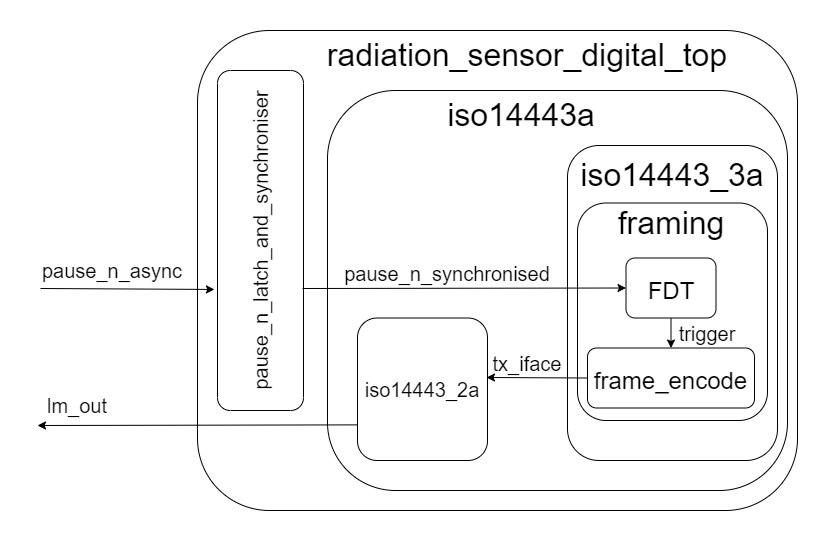
\includegraphics[width=0.8\textwidth]{./img/fdt_path3.drawio}
  \caption{La ruta del FDT en este trabajo.}
  \label{fig:fdt_path}
\end{figure}

Las entradas y salidas son descritas en el \tabref{tab:ports_fdt}.

\begin{table}[htb]
  \centering
  \tablezebra
  \begin{tabulary}{\linewidth}{l|l|L}
    \setcounter{rownum}{0}
    \textbf{Nombre}&\textbf{Dirección}&\textbf{Descripción} \\
    \hline
    clk&Entrada&Reloj. \\
    rst\_n&Entrada&Reset activo bajo. \\
    pause\_n\_synchronised&Entrada&Pausa sincronizada. \\
    last\_rx\_bit&Entrada&Último bit transmitido por el PCD. \\
    trigger&Salida&Señal de habilitación para comenzar la transmisión de la respuesta. \\
  \end{tabulary}
  \caption{Entradas y Salidas del módulo \textbf{FDT}.}
  \label{tab:ports_fdt}
\end{table}

La implementación de este módulo consiste en un detector de flancos ascendentes y un contador. El contador es reseteado a cero cada vez que un flanco ascendente es detectado en la entrada \textit{pause\_n\_synchronised}. Cuándo el contador llega al valor adecuado, calculado con la entrada \textit{last\_rx\_bit} y el parámetro \textit{TIMING\_ADJUST}, la salida \textit{trigger} es pulsada para un ciclo del reloj, y el contador es desactivado hasta que la próxima pausa es detectada.

Para verificar este módulo el banco de prueba instancia el DUT con el parámetro \textit{TIM\-ING\_ADJUST} = 6. Este valor es arbitrario, ya que en este banco de prueba no es necesario compensar por retrasos externos. El valor 6 fue elegido porque es el valor usado en la síntesis de este trabajo. Después hay un bloque de código que mide el tiempo entre el último flanco ascendente de la entrada \textit{pause\_n\_synchronised} y la activación de la salida \textit{trigger}, verificando que es precisamente el número de picosegundos esperados. Las pruebas son:

\begin{itemize}
  \item Verifica que si no hay pausas la señal \textit{trigger} no se activa.
  \item Verifica el FDT cuando la entrada \textit{last\_bit} es ‘0’, mediante una sola pausa.
  \item Verifica que si no hay más pausas la señal \textit{trigger} no se activa una segunda vez.
  \item Verifica el FDT cuando la entrada \textit{last\_bit} es ‘1’, mediante una sóla pausa.
  \item Envía un número aleatorio de pausas con un tiempo aleatorio entre cada una, y verifica que la señal \textit{trigger} sólo se activa después de la última pausa, y que el FDT es correcto.
\end{itemize}

El informe de cobertura da un resultado de 98\% por el DUT. La única parte que falta cobertura es una condición imposible de ocurrir.

% CRC_A
\FloatBarrier
\subsubsection{CRC\_A}

Este módulo calcula el CRC16 definido por el polinomio $x^{16} + x^{12} + x^{5} + 1$ y el valor inicial 0x6363, por una serie de bits. Esta implementación está diseñada para ser utilizada por tramas de recepción y de transmisión, por lo tanto no usa una interfaz. Las salidas y entradas son descritas en el \tabref{tab:ports_crc_a}.

La implementación usa un Registro de Desplazamiento con Realimentación Lineal (LFSR, por sus siglas en Inglés) y es basada en el código generado mediante un generador de LFSRs por CRCs~\cite{crcgen}. Un LFSR es un registro de desplazamiento pero unos de los bits son realimentados con el XOR de otros bits y la entrada. Para calcular el CRC16 con el polinomio definido en la norma, los bits con realimentación son los de índices: 0, 5 y 12. La \figref{fig:crc_lfsr} muestra el LFSR. Las operaciones para calcular los bits con realimentación son:

{%
  \setlength{\abovedisplayskip}{-3pt}
  \setlength{\belowdisplayskip}{\abovedisplayskip}
  \setlength{\abovedisplayshortskip}{0pt}
  \setlength{\belowdisplayshortskip}{0pt}
  \begin{align*}
    \text{lfsr[12]} &= \text{lfsr[15] XOR lfsr[11] XOR data} \\
    \text{lfsr[5]}  &= \text{lfsr[15] XOR lfsr[4] XOR data} \\
    \text{lfsr[0]}  &= \text{lfsr[15] XOR data}  \\
  \end{align*}
}%

Cuándo la entrada \textit{start} es ‘1’, el registro \textit{lfsr} es asignado el valor 0x6363. Cuándo la entrada \textit{sample} es ‘1’ el valor del registro es actualizado con el algoritmo descrito arriba. La salida \textit{crc} es asignado el valor del registro \textit{lfsr}.

\begin{table}[htb]
  \centering
  \tablezebra
  \begin{tabulary}{\linewidth}{l|l|L}
    \textbf{Nombre}&\textbf{Dirección}&\textbf{Descripción} \\
    \hline
    clk&Entrada&Reloj. \\
    rst\_n&Entrada&Reset activo bajo. \\
    start&Entrada&Comenzar un nuevo cálculo. \\
    data&Entrada&Próximo bit. \\
    sample&Entrada&El dato es válida. \\
    crc[15:0]&Salida&Resultado. \\
  \end{tabulary}
  \caption{Entradas y Salidas del módulo \textbf{CRC\_A}.}
  \label{tab:ports_crc_a}
\end{table}

\begin{figure}[htb]
  \centering
  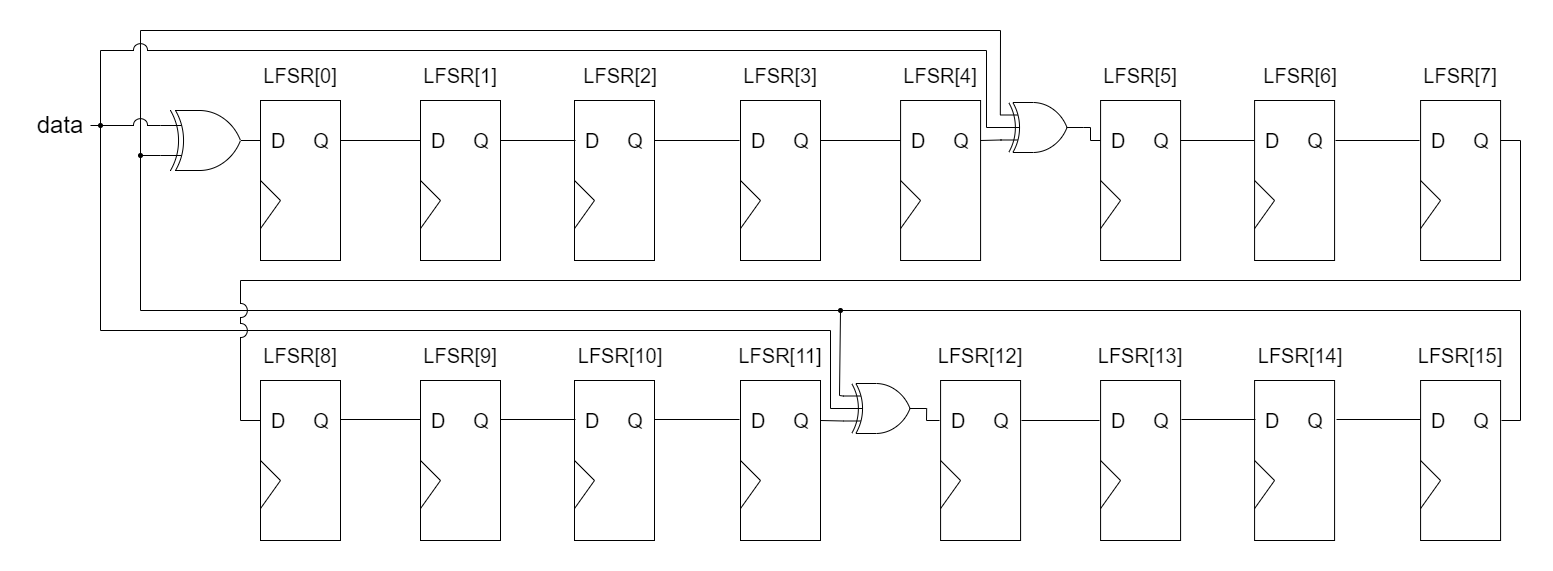
\includegraphics[width=1.0\textwidth]{./img/crc_a_lfsr}
  \caption{El LFSR del módulo \textbf{CRC\_A}.}
  \label{fig:crc_lfsr}
\end{figure}

El banco de prueba para este módulo calcula el CRC de varias series de bytes, mediante dos métodos: con otra implementación del LFSR, y mediante un algoritmo que opera sobre bytes en vez de bits. La implementación de este algoritmo de bytes es provisto en el apéndice B de la parte tres de la norma~\cite{iso14443-3}. Estos dos resultados son comparados con la salida del DUT en dos aserciones. Además el apéndice B de la norma específica los CRCs por dos series de bits. Estas series de bits son verificadas como descrita arriba, y también los resultados son comparados con los especificados en la norma. Las series de bytes probados son:

\begin{itemize}
  \item Sin data: El CRC es el valor inicial 0x6363.
  \item \{0x00, 0x00\}: Especificado en la norma con CRC 0x1EA0.
  \item \{0x12, 0x34\}: Especificado en la norma con CRC 0xCF26.
  \item Mil transacciones aleatorias entre 0 y 10 bytes enteros.
\end{itemize}

El informe de cobertura da un resultado de 100\% por este banco de prueba.

% crc_control
\FloatBarrier
\subsubsection{crc\_control}

Este módulo instancia el módulo \textbf{CRC\_A} y lo usa para verificar los CRCs de tramas recibidas y para calcular los CRCs de tramas a transmitir. Las entradas y salidas son descritas en el \tabref{tab:ports_crc_control}. Este módulo contiene un monitor por la \textit{rx\_interface} y uno por la \textit{tx\_interface}. En este caso el término “monitor” se refiere a un modport en las interfaces dónde todas las señales son entradas. No se debe confundir con los monitores usados en los bancos de pruebas.

\begin{table}[htb]
  \centering
  \tablezebra
  \begin{tabulary}{\linewidth}{l|l|L}
    \textbf{Nombre}&\textbf{Dirección}&\textbf{Descripción} \\
    \hline
    clk&Entrada&Reloj. \\
    rst\_n&Entrada&Reset activo bajo. \\
    rx\_iface&Entrada&Monitor por la \textit{rx\_interface}. \\
    rx\_crc\_ok&Salida&Indica si el CRC de la última trama tiene un CRC válido. \\
    tx\_iface&Entrada&Monitor por la \textit{tx\_interface}. \\
    tx\_append\_crc&Entrada&Calcular el CRC para esta trama de transmisión \\
    fdt\_trigger&Entrada&La señal de habilitación de la transmisión de una trama, desde el módulo FDT. \\
    crc[15:0]&Salida&El resultado \\
  \end{tabulary}
  \caption{Entradas y Salidas del módulo \textbf{crc\_control}.}
  \label{tab:ports_crc_control}
\end{table}

Una propiedad de este algoritmo de CRC es: si se agrega el CRC de una serie de bits al final de esa serie, el CRC de la nueva serie de bits es cero. Por lo tanto para verificar la integridad de una trama recibida, es suficiente comprobar que el CRC calculado en este módulo es cero.

La entrada \textit{start} del módulo \textbf{CRC\_A} es pulsado al detectar el principio de una trama en una de las interfaces. Esto causa que el módulo \textbf{CRC\_A} reinicie su LFSR. En el caso de tramas recibidas desde el PCD el principio de una trama es indicado con la señal \textit{rx\_iface.soc}. En el caso de tramas a transmitir el principio de una trama es indicado cuando las entradas \textit{fdt\_trigger}, y \textit{tx\_iface.data\_valid} están en ‘1’s, también en este caso solo se calcula el CRC cuándo la entrada \textit{tx\_append\_crc} está en ‘1’. La entrada \textit{sample} del módulo \textbf{CRC\_A} es pulsado por cada bit de la trama, lo que ocurre cuándo una de las señales \textit{rx\_iface.data\_valid} o \textit{tx\_iface.req} están en ‘1’. Este módulo no es responsable de agregar CRCs a las respuestas, eso ocurre en el módulo \textbf{frame\_encode}. La salida \textit{rx\_crc\_ok} es ‘1’ cuando el resultado del módulo \textbf{CRC\_A} es cero.

El banco de prueba por este módulo consiste en tres controladores: \textbf{RxBitIfaceDriver}, \textbf{TxBitIfaceSourceDriver} y \textbf{TxBitIfaceSinkDriver}. El controlador  \textbf{TxBitIfaceSinkDriver} es necesario para manejar la señal \textit{tx\_iface.req} porque el DUT no contiene un sumidero. Varias tramas son enviadas sobre ambos interfaces, y las salidas del DUT \textit{crc} y \textit{rx\_crc\_ok} son verificadas mediante aserciones:

\begin{itemize}
  \item Verifica que la salida \textit{rx\_crc\_ok} es como esperado al final de una trama de recepción.
  \item Verifica que la salida \textit{rx\_crc\_ok} no cambia después del fin de una trama.
  \item Verifica que la salida \textit{crc} es igual al CRC esperado al final de una trama de transmisión.
  \item Verifica que la salida \textit{crc} no cambia después del fin de una trama.
  \item Verifica que la salida \textit{crc} no cambia mientras un indicador \textit{check\_crc\_stable} está ‘1’.
  \item Verifica que \textit{rx\_crc\_ok} es ‘1’ cuando y sólo cuando la salida \textit{crc} es cero.
\end{itemize}

Las pruebas ejecutados son:

\begin{itemize}
  \item Enviar tres tramas sobre la \textit{rx\_iface}: \{0x00, 0x00, 0xA0, 0x1E\}, \{0x12, 0x34, 0x26, 0xCF\} y \{0x63, 0x63\}. Estas tramas son las series de bits con sus CRCs especificados en el apéndice B de la norma~\cite{iso14443-3}.
  \item Enviar mil tramas sobre la \textit{rx\_iface} con sus CRC agregados.
  \item Enviar mil tramas sobre la \textit{rx\_iface} con sus CRC agregados y un bit de la trama corrompido.
  \item Enviar dos tramas sobre la \textit{tx\_iface}: \{0x00, 0x00\}, y \{0x12, 0x34\}, para verificar la salida \textit{crc} es 0x1EA0 y 0xCF26 respectivamente, como especificado en el apéndice B de la norma.
  \item Enviar mil tramas sobre la \textit{tx\_iface} y verificar que la salida \textit{crc} es como se espera en cada caso.
\end{itemize}

El informe de cobertura da un resultado de 100\% por el DUT.

% serialiser
\FloatBarrier
\subsubsection{serialiser}

Este módulo es parecido al módulo \textbf{deserialiser} pero al revés, convierte tramas de bytes a tramas de bits para transmisión. Las salidas y entradas son descritas en el \tabref{tab:ports_serialiser}.

Este módulo espera por el principio de una trama, lo que pasa cuándo la entrada \textit{in\_iface.data\_valid} está en ‘1’ y después fija la salida \textit{out\_iface.data\_valid} en ‘1’ y la salida \textit{out\_iface.data} en el valor del primer bit de la entrada \textit{in\_iface.data}. Cuando el módulo conectado a la fuente \textit{out\_iface} pide el siguiente bit mediante la señal \textit{out\_iface.req}, la salida \textit{out\_iface.data} se actualiza. Después de haber enviado el último bit del byte, la salida \textit{out\_iface.last\_bit\_in\_byte} pasa a ‘1’, y otro byte es pedido mediante la salida \textit{in\_iface.req}. Ese proceso continúa hasta el final de la trama. Debido a que las respuestas pueden comenzar con un byte parcial en el caso de tramas de anticolisión, la entrada \textit{in\_iface.data\_bits} se usa para determinar el número de bits en el primer byte.


\begin{table}[htb]
  \centering
  \tablezebra
  \begin{tabulary}{\linewidth}{l|l|L}
    \textbf{Nombre}&\textbf{Dirección}&\textbf{Descripción} \\
    \hline
    clk&Entrada&Reloj. \\
    rst\_n&Entrada&Reset activo bajo. \\
    in\_iface&Entrada&Sumidero para la \textit{tx\_interface}. \\
    out\_iface&Salida&Fuente para la \textit{tx\_interface}. \\
  \end{tabulary}
  \caption{Entradas y Salidas del módulo \textbf{serialiser}.}
  \label{tab:ports_serialiser}
\end{table}

El banco de prueba para este módulo consiste en dos controladores y un monitor: un \textbf{TxByteIfaceSourceDriver} por la entrada \textit{in\_iface}, un \textbf{TxBitIfaceSinkDriver} por la salida \textit{out\_iface}, y un \textbf{TxBitIfaceMonitor} por la salida \textit{out\_iface}. Para verificar el comportamiento del DUT, transacciones de bytes son generadas y enviadas. Después las transacciones enviadas son convertidas a transacciones de bits, y comparadas con las recibidas por el monitor. Hay dos pruebas: Enviar 16 transacciones de tamaños 1 a 16 bits en orden, y envíar mil transacciones de tamaños aleatorios.

El informe de cobertura da un resultado de 100\% por el DUT.

% frame_encode
\FloatBarrier
\subsubsection{frame\_encode}

Este módulo es responsable de agregar el CRC16 y los bits de paridad a las respuestas. Además solo comienza envíar la trama cuando está activado mediante una entrada \textit{fdt\_trigger} que viene del módulo \textbf{FDT}. Las salidas y entradas son descritas en el \tabref{tab:ports_frame_encode}.

\begin{table}[htb]
  \centering
  \tablezebra
  \begin{tabulary}{\linewidth}{l|l|L}
    \setcounter{rownum}{0}
    \textbf{Nombre}&\textbf{Dirección}&\textbf{Descripción} \\
    \hline
    clk&Entrada&Reloj. \\
    rst\_n&Entrada&Reset activo bajo. \\
    fdt\_trigger&Entrada&Señal para activar el envío de la respuesta. \\
    in\_iface&Entrada&Sumidero de la \textit{tx\_interface}. \\
    append\_crc&Entrada&Indica que la respuesta tiene CRC. \\
    crc[15:0]&Entrada&CRC. \\
    out\_iface&Salida&Fuente de la \textit{tx\_interface}. \\
  \end{tabulary}
  \caption{Entradas y Salidas del módulo \textbf{frame\_encode}.}
  \label{tab:ports_frame_encode}
\end{table}

La implementación espera la señal de habilitación desde el módulo \textbf{FDT}. En ese momento si hay una trama lista para enviar, indicado con la entrada \textit{in\_iface.data\_valid}, comienza reenviar la trama sobre la \textit{out\_iface}. El bit de paridad por cada byte es calculado en la misma manera del módulo \textbf{frame\_decode}. Cuándo la entrada \textit{in\_iface.last\_bit\_in\_byte} está en ‘1’, indicando el último bit en el byte actual, el bit de paridad calculado es enviado. Después del fin de la trama, si la entrada \textit{append\_crc} está en ‘1’, el CRC y su bits de paridad son enviados.

El banco de prueba consiste en: el controlador de fuente \textbf{TxBitIfaceSourceDriver} por la \textit{in\_iface}, el controlador de sumidero \textbf{TxBitIfaceSinkDriver} y el monitor \textbf{TxBitIfaceMonitor} por la \textit{out\_iface}. Para verificar el comportamiento del DUT, transacciones son generadas y enviadas. Por cada prueba, si la trama tiene un CRC, está agregado a la transacción. Los bits de paridad siempre son agregados. Esta nueva transacción es comparada con la trama detectada por el monitor. Debido a que el DUT solo comienza enviar una trama cuándo su entrada \textit{fdt\_trigger} está ‘1’, esa señal es pulsada un número de ciclos aleatorios después de que la transacción fue enviada al controlador. Las pruebas son:

\begin{itemize}
  \item Envía cien tramas, pero no pulsa la señal \textit{fdt\_trigger}, y verifica que el monitor no recibe ninguna transacción.
  \item Pulsa \textit{fdt\_trigger} sin envíar una transacción y verifica que el monitor no recibe ninguna transacción.
  \item Envía tramas de tamaño entre uno y ocho bits, sin CRCs.
  \item Envía mil tramas de tamaño aleatorio, sin CRC.
  \item Envía mil tramas cada una con un número de bytes entero, con CRC.
\end{itemize}

El informe de cobertura por el DUT da un resultado de 98\%. La única parte que falta cobertura es una condición imposible de ocurrir.

% framing
\FloatBarrier
\subsubsection{framing}

Este módulo simplemente instancia los siguientes módulos: \textbf{frame\_decode}, \textbf{deserialiser}, \textbf{FDT}, \textbf{crc\_control}, \textbf{deserialiser} y \textbf{frame\_encode}, como se muestra la \figref{fig:framing}. Las entradas y salidas están descritas en el \tabref{tab:ports_framing}.

\begin{figure}[htb]
  \centering
  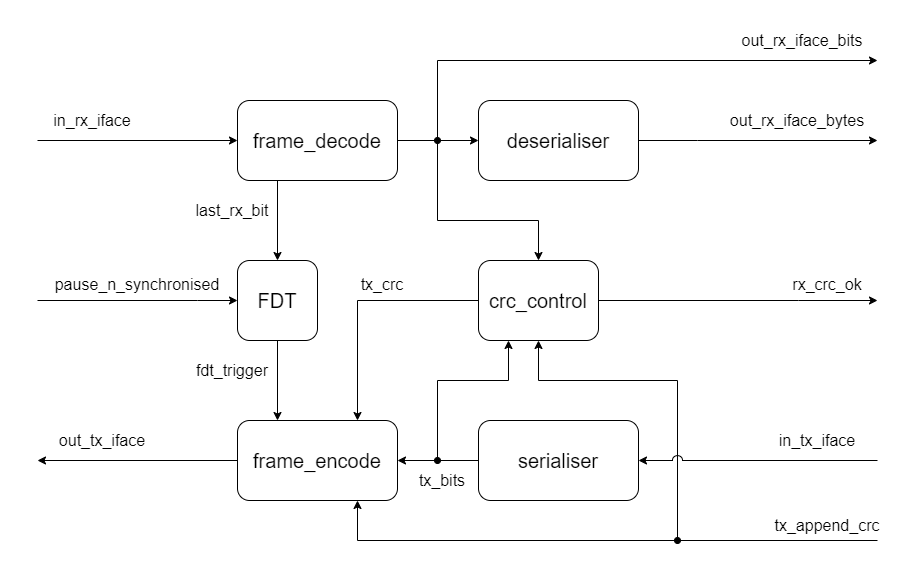
\includegraphics[width=1.0\textwidth]{./img/framing.drawio}
  \caption{Diagrama en bloques del módulo \textbf{framing}.}
  \label{fig:framing}
\end{figure}

\begin{table}[htb]
  \centering
  \tablezebra
  \begin{tabulary}{\linewidth}{l|l|L}
    \textbf{Nombre}&\textbf{Dirección}&\textbf{Descripción} \\
    \hline
    clk&Entrada&Reloj. \\
    rst\_n&Entrada&Reset activo bajo. \\
    pause\_n\_synchronised&Entrada&Pausa, activa bajo, sincronizada. \\
    in\_rx\_iface&Entrada&Sumidero de bits por la \textit{rx\_interface}. \\
    out\_rx\_iface\_bytes&Salida&Fuente de bytes por la \textit{rx\_interface}. \\
    out\_rx\_iface\_bits&Salida&Fuente de bits por la \textit{rx\_interface}. \\
    rx\_crc\_ok&Salida&Indica que la última trama recibida tiene CRC válido. \\
    in\_tx\_iface&Entrada&Sumidero de bytes por la \textit{tx\_interface}. \\
    tx\_append\_crc&Entrada&Indica que la respuesta debe tener CRC. \\
    out\_tx\_iface&Salida&Fuente de bits por la \textit{tx\_interface}. \\
  \end{tabulary}
  \caption{Entradas y Salidas del módulo \textbf{framing}.}
  \label{tab:ports_framing}
\end{table}

\FloatBarrier

Para la ruta de recepción el flujo de datos es:

\begin{itemize}
  \item Los bits de paridad están verificados y quitados.
  \item El CRC es verificado.
  \item La trama de bits es convertida a una trama de bytes.
  \item El temporizador del FDT comienza a contar después del último flanco ascendente de la pausa.
\end{itemize}

Hay dos salidas por las tramas recibidas desde el PCD, \textit{out\_rx\_iface\_bytes} y \textit{out\_rx\_iface\_bits}. La fuente de bits es para facilitar la comparación del UID en tramas de anticolisión en el módulo \textbf{initialisation}. Este tema es descrito más en la \secref{sec:initialisation}{initialisation}.

Para la ruta de transmisión el flujo de datos es:

\begin{itemize}
  \item La transmisión comienza cuando el temporizador del FDT vence.
  \item Las tramas de bytes son convertidas a tramas de bits.
  \item Los bits de paridad son insertados.
  \item El CRC es calculado y agregado, incluyendo sus bits de paridad, si es pedido con la entrada \textit{tx\_append\_crc}.
\end{itemize}

Este módulo tiene un parámetro \textit{FDT\_TIMING\_ADJUST} que especifica el retardo en la ruta del FDT externo a este módulo. El módulo \textbf{frame\_decode} introduce un ciclo de retardo en la transmisión de la respuesta, por lo tanto el valor pasado al parámetro \textit{TIMING\_ADJUST} del módulo \textbf{FDT} es \textit{FDT\_TIMING\_ADJUST} + 1.

El banco de prueba para este módulo consiste en:

\begin{itemize}
  \item Un controlador \textbf{RxBitIfaceDriver} por la \textit{in\_rx\_iface}.
  \item Un monitor \textbf{RxBitIfaceMonitor} por la \textit{out\_rx\_iface\_bits}.
  \item Un monitor \textbf{RxByteIfaceMonitor} por la \textit{out\_rx\_iface\_bytes}.
  \item Un controlador de fuente \textbf{TxByteIfaceSourceDriver} por la \textit{in\_tx\_iface}.
  \item Un controlador de sumidero \textbf{TxBitIfaceSinkDriver} por la \textit{out\_tx\_iface}.
  \item Un monitor \textbf{TxBitIfaceMonitor} por la \textit{out\_tx\_iface}.
\end{itemize}

Para simular la recepción de una trama desde el PCD hay una tarea \textbf{send\_rx\_frame()} que construye una transacción aleatoriamente con el número de bits especificado en un argumento. Si tiene un número de bytes entero, el CRC es calculado y agregado. Después los bits de paridad son insertados. Otro argumento especifica si la trama debería contener un error, y que tipo de error. Los tipos de errores son: bit de paridad equivocado, falta el último bit de paridad, CRC equivocado, y un error en la trama enviada mediante la señal \textit{in\_rx\_iface.error}. Las transacciones recibidas por los dos monitores son comparadas con las esperadas. Hay una aserción concurrente que verifica que la salida \textit{rx\_crc\_ok} es como esperado por cada trama.

La ruta de transmisión es parecida. La tarea \textbf{send\_tx\_frame()} arma una transacción de bytes con el número de bits especificado en un argumento. La transacción recibida por el monitor es comparada con la enviada. El DUT sólo comienza transmitir una trama cuando el temporizador del módulo \textbf{FDT} vence. Para comenzar este temporizador se requiere al menos un flanco ascendente en la entrada \textit{pause\_n\_synchronised}. Por lo tanto esta tarea pulsa esa señal, después de haber pasado una transacción al controlador.

Como en el banco de prueba para el módulo \textbf{FDT}, el tiempo entre el último flanco ascendente de la pausa y el principio de la transmisión de la respuesta es medido y verificado.

Las pruebas son listadas acá, cada uno es repetida mil veces:

\begin{itemize}
  \item Envía una trama sobre la \textit{in\_rx\_iface} de número de bytes entero, con CRC.
  \item Envía una trama sobre la \textit{in\_rx\_iface} terminando con un byte parcial, sin CRC.
  \item Envía una trama sobre la \textit{in\_rx\_iface} de número de bytes entero, con CRC equivocado.
  \item Envía una trama sobre la \textit{in\_rx\_iface} con un bit de paridad equivocado.
  \item Envía una trama sobre la \textit{in\_rx\_iface} que falta su último bit de paridad.
  \item Envía una trama sobre la \textit{in\_rx\_iface} con un error mediante la señal \textit{in\_rx\_iface.error}.
  \item Envía una trama sobre la \textit{in\_tx\_iface} sin CRC.
  \item Envía una trama sobre la \textit{in\_tx\_iface} de número de bytes enteros con CRC.
  \item Envía una trama sobre la \textit{in\_rx\_iface} y después una trama sobre la \textit{in\_tx\_iface} como una respuesta.
\end{itemize}

El informe de cobertura por el DUT da un resultado de 100\%.

% routing
\FloatBarrier
\subsubsection{routing}

La norma ISO/IEC 14443 divide las definiciones de las tramas entre las partes tres y cuatro de la norma, y el diseño de este núcleo IP siguiendo esta división, procesa esas tramas en módulos distintos. La norma específica cuáles tramas son aceptadas en cada estado de la PICC, la \figref{fig:14443-3-state-machine} muestra esto. En los estados: IDLE, READY, HALT y READY*, la PICC solo soporta las tramas de inicialización y anticolisión. En el estado PROTOCOL, la PICC solo soporta las tramas definidas en la parte cuatro de la norma. En los estados: ACTIVE y ACTIVE*, la PICC puede recibir la trama de inicialización HLTA o la trama RATS de la parte cuatro de la norma. Este módulo es diseñado para dirigir tramas recibidas desde el PCD a los módulos que correspondan: \textbf{initialisation} y \textbf{iso14443\_4a} dependiendo en el estado actual de la PICC, y además dirige las respuestas generadas desde cada módulo. Las entradas y salidas están descritas en el \tabref{tab:ports_routing}.

\begin{table}[htb]
  \centering
  \tablezebra
  \begin{tabulary}{\linewidth}{l|l|L}
    \textbf{Nombre}&\textbf{Dirección}&\textbf{Descripción} \\
    \hline
    route\_rx\_to\_initialisation&Entrada&Dirigir tramas recibidas al módulo \textbf{initialisation}. \\
    route\_rx\_to\_14443\_4&Entrada&Dirigir tramas recibidas al módulo \textbf{iso14443\_4a}. \\
    route\_tx\_from\_14443\_4&Entrada&Aceptar respuestas desde el módulo \textbf{iso14443\_4a} (valor ‘1’), o desde el módulo \textbf{initialisation} (valor ‘’0’). \\
    in\_rx\_iface&Entrada&Sumidero para la \textit{rx\_interface}. \\
    out\_rx\_iface\_init&Salida&Fuente para la \textit{rx\_interface}, conectado al módulo \textbf{initialisation}. \\
    out\_rx\_iface\_14443\_4&Salida&Fuente para la \textit{rx\_interface}, conectado al módulo \textbf{iso14443\_4a}. \\
    in\_tx\_iface\_init&Entrada&Sumidero para la \textit{tx\_interface}, desde el módulo \textbf{initialisation}. \\
    in\_tx\_append\_crc\_init&Entrada&La respuesta desde el módulo \textbf{initialisation} debe tener CRC agregado. \\
    in\_tx\_iface\_14443\_4&Entrada&Sumidero para la \textit{tx\_interface}, desde el módulo \textbf{iso14443\_4a}. \\
    in\_tx\_append\_crc\_14443\_4&Entrada&La respuesta desde el módulo \textbf{iso14443\_4a} debe tener CRC agregado. \\
    out\_tx\_iface&Salida&Fuente para la \textit{tx\_interface}. \\
    out\_tx\_append\_crc&Salida&La respuesta enviada debe tener CRC agregado. \\
  \end{tabulary}
  \caption{Entradas y Salidas del módulo \textbf{routing}.}
  \label{tab:ports_routing}
\end{table}

La implementación es un circuito combinatorio para evitar el uso de registros y reducir el área del diseño. La ruta de recepción consiste en una entrada: \textit{in\_rx\_iface}, dos salidas: \textit{out\_rx\_iface\_init} y \textit{out\_rx\_iface\_14443\_4}, y dos señales de control: \textit{route\_rx\_to\_initialisation} y \textit{route\_rx\_to\_14443\_4}. Las señales \textit{in\_rx\_iface.data} y \textit{in\_rx\_iface.data\_bits} simplemente son conectadas a las señales correspondientes de las dos salidas. Las demás de las señales: \textit{error}, \textit{soc}, \textit{eoc}, y \textit{data\_valid} pasan por compuertas ANDs con la señal de control correspondiente, como se muestra la \figref{fig:routing_rx}. De esta forma, si una salida no está activada los indicadores en la interfaz de esa salida serían ‘0’.

\begin{figure}[htb]
  \centering
  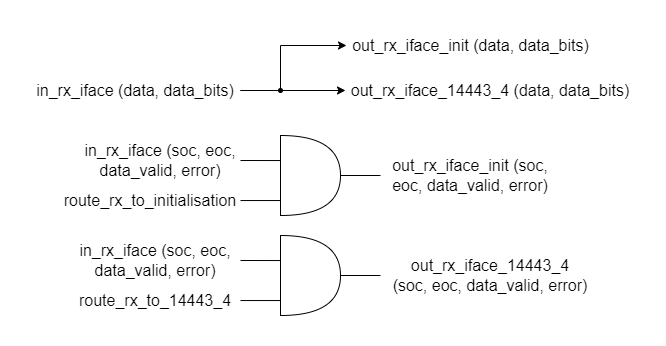
\includegraphics[width=0.8\textwidth]{./img/routing_rx.drawio}
  \caption{La ruta de recepción para las señales en el módulo \textbf{routing}.}
  \label{fig:routing_rx}
\end{figure}

La ruta de transmisión tiene dos entradas: \textit{in\_tx\_iface\_init} y \textit{in\_tx\_iface\_14443\_4}, una salida: \textit{out\_tx\_iface}, y una señal de control: \textit{route\_tx\_from\_14443\_4}. Cuando \textit{route\_tx\_from\_14443\_4} está ‘0’, respuestas son dirigidas desde la entrada \textit{in\_tx\_iface\_init}, y cuándo está ‘1’ las respuestas son dirigidas desde la entrada \textit{in\_tx\_iface\_14443\_4}. Las señales \textit{in\_tx\_iface\_init.req} y \textit{in\_tx\_iface\_14443\_4.req} deben ser ‘0’ cuando su entrada está desactivada. Por lo tanto un par de compuertas AND son usadas. Las otras señales son conectadas mediante un multiplexor. La \figref{fig:routing_tx} muestra está implementación.

\begin{figure}[htb]
  \centering
  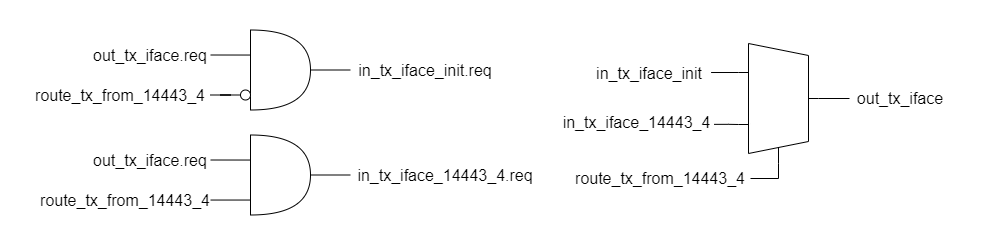
\includegraphics[width=1.0\textwidth]{./img/routing_tx.drawio}
  \caption{La ruta de transmisión en el módulo \textbf{routing}.}
  \label{fig:routing_tx}
\end{figure}

El banco de prueba por este módulo simplemente fija las señales de control en los modos definidos abajo, cambia todas las entradas aleatoriamente y verifica que todas las salidas son como esperadas. Este proceso es repetido diez mil veces por cada uno de estos modos:

\begin{itemize}
  \item Rx solo a \textbf{initialisation}, Tx desde \textbf{initialisation}.
  \item Rx solo a \textbf{iso14443\_4a}, Tx desde \textbf{iso14443\_4a}.
  \item Rx a \textbf{initialisation} y \textbf{iso14443\_4a}, Tx desde \textbf{initialisation}.
  \item Rx a \textbf{initialisation} y \textbf{iso14443\_4a}, Tx desde \textbf{iso14443\_4a}.
\end{itemize}

El informe de cobertura da el DUT un resultado de 100\%.

% initialisation
\FloatBarrier
\subsubsection{initialisation}
\label{sec:initialisation}

Este módulo es el primero que actúa sobre las tramas recibidas y genera las respuestas requeridas por la norma. Las tramas soportadas son las de inicialización y anticolisión: REQA, WUPA, ANTICOLLISION, SELECT, y HLTA. Las salidas y entradas son descritas en el \tabref{tab:ports_initialisation}. Este es un módulo parametrizado, cuyos parámetros son descritos en el \tabref{tab:params_initialisation}.

\begin{table}[htb]
  \centering
  \tablezebra
  \begin{tabulary}{\linewidth}{l|l|L}
    \textbf{Nombre}&\textbf{Dirección}&\textbf{Descripción} \\
    \hline
    clk&Entrada&Reloj. \\
    rst\_n&Entrada&Reset activo bajo. \\
    uid\_variable&Entrada&Bits menos significativos del UID. \\
    rx\_iface&Entrada&Sumidero de bytes por la \textit{rx\_interface}. \\
    rx\_iface\_bits&Entrada&Sumidero de bits por la \textit{rx\_interface}. \\
    rx\_crc\_ok&Entrada&Los últimos dos bytes de la trama recibida son un CRC válido. \\
    tx\_iface&Salida&Fuente de bytes por la \textit{tx\_interface}. \\
    tx\_append\_crc&Salida&La respuesta debe tener un CRC agregado. \\
    iso14443\_4a\_deselect&Entrada&El bloque ISO/IEC 14443-4A recibió el bloque estándar S(DESELECT). \\
    iso14443\_4a\_rats&Entrada&El bloque ISO/IEC 14443-4A recibió el mensaje RATS. \\
    iso14443\_4a\_tag\_active&Salida&La PICC está en el estado ACTIVE. \\
    route\_rx\_to\_initialisation&Salida&Tramas de recepción deberían estar dirigidas a este módulo. \\
    route\_rx\_to\_14443\_4a&Salida&Tramas de recepción deberían estar dirigidas al módulo \textbf{iso14443\_4a}. \\
    route\_tx\_from\_14443\_4a&Salida&El módulo \textbf{iso14443\_4a} es la fuente de las respuestas (valor ‘1’), o este módulo es la fuente (valor ‘0’). \\
  \end{tabulary}
  \caption{Entradas y Salidas del módulo \textbf{initialisation}.}
  \label{tab:ports_initialisation}
\end{table}

\begin{table}[htb]
  \centering
  \tablezebra
  \begin{tabulary}{\linewidth}{l|l|L}
    \setcounter{rownum}{0}
    \textbf{Nombre}&\textbf{Tipo}&\textbf{Descripción} \\
    \hline
    UID\_SIZE&UIDSize (enum)&La PICC tiene un UID simple, doble o triple. \\
    UID\_INPUT\_BITS&int&El ancho de la entrada \textit{uid\_variable}. \\
    UID\_FIXED&logic [] (un vector)&Bits más significativos del UID. \\
  \end{tabulary}
  \caption{Parámetros del módulo \textbf{initialisation}.}
  \label{tab:params_initialisation}
\end{table}

Cómo descrito en la \secref{sec:introduction_iso14443-3}{ISO/IEC 14443-3}, durante el proceso de inicialización hay un lazo de anticolisión, dónde el UID es dividido en hasta tres partes y el PCD tiene que realizar el proceso de anticolisión y enviar una trama SELECT para cada parte del UID en turno para que la PICC transiciona al estado READY o READY*. Esto es conocido como los niveles cascadas.

El UID de la PICC es la concatenación del parámetro \textit{UID\_FIXED} y la entrada \textit{uid\_var\-iable}, el número de bits total y el número de niveles cascadas dependen en el parámetro \textit{UID\_SIZE}:

\begin{description}[labelwidth=3.8cm]
    \item [UIDSize\_SINGLE:] 32 bits, 1 nivel cascada.
    \item [UIDSize\_DOUBLE:] 56 bits, 2 niveles cascadas.
    \item [UIDSize\_TRIPLE:] 80 bits, 3 niveles cascadas.
\end{description}

Un bloque “generate” es usado para partir el UID y agregar las tags cascadas al tiempo de elaboración, de la forma que muestra la \figref{fig:cascade_levels}. Hay una señal \textit{current\_cascade\_level} que indica en qué lazo de anticolisión la PICC está actualmente. Usando esa señal y un mux, una señal \textit{current\_cascade\_uid\_data} está asignada con los datos correspondientes para el nivel de cascada actual. Finalmente cada nivel de cascada termina con un byte BCC (Block Check Character), lo que es el XOR de los últimos cuatros bytes, este valor es calculado e incluido en la señal \textit{current\_cascade\_uid\_data}. Esta señal es usada con las tramas: ANTICOLLISION y SELECT para comparar el UID enviado en la trama con lo de esta PICC. En el caso de la trama ANTICOLLISION, esta señal también es usada para armar la respuesta. La \figref{fig:init_cascade_levels} muestra el circuito implementado para una PICC con UID doble.

Las tramas recibidas desde el PCD son guardadas en un buffer. La trama más larga es la SELECT lo que tiene siete bytes más dos bytes de CRC. Debido a que el CRC es verificado en el módulo \textbf{framing}, no es necesario guardar el CRC en el buffer, así el tamaño del buffer implementado es siete bytes. Si la señal \textit{in\_rx\_iface\_bytes.error} indica un error los demás datos de la trama son ignorados.

La implementación de este módulo incluye una máquina de estados basada en la especificación de la parte tres de la norma. Esta máquina de estados se muestra en la \figref{fig:14443-3-state-machine}. Debido a que las tramas: RATS, y S(DESELECT) son procesadas en el módulo \textbf{iso14443\_4a}, las transiciones correspondientes son realizadas cuando ese módulo indica la recepción de esas tramas mediante las entradas: \textit{iso14443\_4a\_rats} y \textit{iso14443\_4a\_deselect}. En el estado ACTIVE si la PICC recibe cualquier trama menos una RATS, esa trama es tratada como un error, y se transiciona al estado IDLE o HALT.

\begin{figure}[htb]
  \centering
  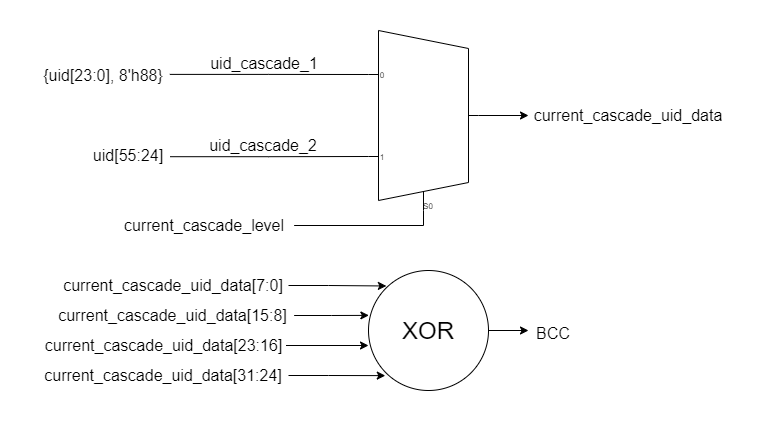
\includegraphics[width=1.0\textwidth]{./img/initialisation_uid.drawio}
  \caption{La implementación de los niveles cascadas por una PICC con UID doble en el módulo \textbf{initialisation}.}
  \label{fig:init_cascade_levels}
\end{figure}

Las respuestas son construidas en un buffer de cinco bytes. Cuando la máquina de estados determina que una respuesta es necesaria, el buffer es llenado con los datos de la respuesta,  y la salida \textit{tx\_iface.data\_valid} se fija en ‘1’ para indicar al sumidero que una respuesta está lista para transmitir. Después, cada vez que la señal \textit{tx\_iface.req} está pulsada, el buffer es desplazado un byte, para transmitir el próximo byte. Cuando no hay más bytes a enviar, la señal \textit{tx\_iface.data\_valid} vuelve a ‘0’ para indicar el fin de la trama. Hay tres respuestas posibles:

\begin{itemize}
  \item ATQA: respuesta a REQA / WUPA. Tiene dos bytes que solo dependen del parámetro: \textit{UID\_SIZE}.
  \item SAK: respuesta a SELECT. Tiene un byte, que depende de si el nivel de cascada actual es la última.
  \item ANTICOLLISION: respuesta a ANTICOLLISION. Tiene entre un bit y cinco bytes del UID, que corresponden a la parte no enviada en la solicitud.
\end{itemize}

\newpage

La \figref{fig:anticollision} muestra la solicitud y la respuesta por la trama ANTICOLLISION. El PCD envía parte de un UID y todas las PICCs quienes UIDs corresponden, responden con los de más de sus UIDs. La trama SELECT es igual a una ANTICOLLISION pero el PCD envía el UID entero y un CRC es agregado. Para determinar si el UID en la solicitud corresponde con el UID de esta PICC es necesario implementar un circuito digital que puede comparar entre cero y cinco bytes y en el caso de que el último byte es un byte parcial, entre 1 y 7 bits de ese byte. El circuito necesario para hacer esa comparación de forma combinatoria es un circuito grande. Una opción mejor y que es usada en esta implementación es comparar cada bit del UID en turno en el momento que es recibido. La entrada \textit{rx\_iface\_bits} existe por esta razón. Después de haber recibido dos bytes de una trama mediante la entrada \textit{rx\_iface\_bytes} como normal, si la data indica que la trama es una ANTICOLLISION o una SELECT, el diseño comienza comparando cada bit recibida sobre la \textit{rx\_iface\_bits} con su UID. Otra ventaja de este método es que se puede construir la respuesta usando un registro de desplazamiento iniciado con el UID completo para el nivel de cascada actual, y desplazándolo con cada bit recibido.

El banco de prueba para este módulo consiste en:

\begin{itemize}
  \item El controlador \textbf{RxBitIfaceDriver} para simular tramas desde el PCD
  \item El módulo \textbf{deserialiser} para convertir la trama de bits a una trama de bytes, esto permite el envío de la misma transacción sobre las dos \textit{rx\_interfaces}.
  \item El monitor \textbf{TxByteIfaceMonitor} para recibir las respuestas.
  \item El controlador de sumidero \textbf{TxByteIfaceSinkDriver} por la \textit{tx\_iface}.
  \item Una secuencia \textbf{InitCommsTbSequence}. Esta es una clase que extiende la secuencia \textbf{CommsTestsSequence}. Esta clase provee funcionalidades específicas (customisations) a este banco de prueba. Las funcionalidades incluyen:
  \begin{itemize}[label=$\circ$]
    \item Una tarea \textbf{do\_reset()}. Esta tarea resetea el DUT a un estado conocido.
    \item Antes de enviar una trama de recepción, actualiza la entrada \textit{rx\_crc\_ok} del DUT para indicar si el CRC de la trama es válido.
    \item Maneja las entradas \textit{iso14443\_4a\_rats} y \textit{iso14443\_4a\_deselect} para simular el módulo \textbf{iso14443\_4a} recibiendo una RATS y una S(DESELCT).
    \item Verifica que la salida \textit{tx\_append\_crc} del DUT es correcta durante el envío de una respuesta.
    \item Verifica el estado actual del DUT después del envío de cada trama.
  \end{itemize}
\end{itemize}

El banco de prueba ejecuta todas las pruebas diez veces, con UIDs diferentes. Dentro de este lazo cada prueba es repetida cien veces. Las pruebas ejecutadas son las pruebas de inicialización definidas en la secuencia \textbf{CommsTestSequence}, y se parten en cuatro grupos:

\begin{itemize}
  \item Pruebas de transiciones de estados. Estas pruebas verifican la implementación de la máquina de estados mostrado en la \figref{fig:14443-3-state-machine}. Cada prueba consiste en los pasos:
  \begin{itemize}
    \item Entra el estado inicial querido.
    \item Envía una trama.
    \item Verifica la respuesta o que no hay respuesta.
    \item Verifica que el DUT está en el estado esperado.
  \end{itemize}
  \item Pruebas con tramas de ANTICOLLISION y SELECT.
  \begin{itemize}
    \item Verifica que las tramas de ANTICOLLISION son procesadas correctamente cuando el UID enviado corresponde a la del DUT.
    \item Verifica que las tramas de ANTICOLLISION y SELECT son procesadas correctamente cuando el UID enviado no corresponde a la del DUT.
  \end{itemize}
  \item Pruebas con tramas que contienen errores de CRC. Verifica que el DUT no responde a tramas que contienen CRCs inválidos, y transiciona al estado IDLE o HALT como es esperado.
  \item Pruebas que verifican que las tramas definidas en la parte cuatro de la norma no son aceptadas cuando la PICC no está en el estado correspondiente. En los estados: IDLE, READY, HALT y READY*, la PICC no debería responder a ninguna de esas tramas, y deberían ser tratadas como errores. En los estados ACTIVE y ACTIVE*, se aplica lo mismo, salvo por la trama RATS.
\end{itemize}

No es posible verificar el comportamiento del diseño entero con una sola simulación. Esto se debe a que el DUT está parametrizado en el tamaño del UID y el valor de este parámetro determina qué circuito es implementado mediante un bloque “generate”. Por lo tanto el banco de prueba también es parametrizado en el tamaño del UID, y una simulación es ejecutada por cada tamaño de UID.

El informe de cobertura por estas tres simulaciones dan resultados por el DUT de: 94\%, 97\% y 97\% por UIDs simples, dobles y triples respectivamente. La diferencia es debido a que algunas partes del circuito no son usadas si solo hay uno o dos niveles cascadas. En el caso del UID triple las partes que faltan cobertura son mayormente casos imposibles de ocurrir (por ejemplo la parte fija del UID falta cobertura de toggle).

% ISO/IEC 14443-3A
\FloatBarrier
\subsubsection{ISO/IEC 14443-3A}

Este módulo instancia los módulos: \textbf{framing}, \textbf{routing} y \textbf{initialisation}, como se muestra en la \figref{fig:iso14443_3a}. Las entradas y salidas son descritas en el \tabref{tab:ports_iso14443_3a}.

\begin{table}[htb]
  \centering
  \tablezebra
  \begin{tabulary}{\linewidth}{l|l|L}
    \setcounter{rownum}{0}
    \textbf{Nombre}&\textbf{Dirección}&\textbf{Descripción} \\
    \hline
    clk&Entrada&Reloj. \\
    rst\_n&Entrada&Reset activo bajo. \\
    uid\_variable&Entrada&Bits menos significativos del UID. \\
    pause\_n\_synchronised&Entrada&Pausa, activa baja, sincronizada. \\
    rx\_iface\_from\_14443\_2a&Entrada&Sumidero de bits de la \textit{rx\_interface}, conectado al módulo \textbf{ios14443\_2a} \\
    tx\_iface\_to\_14443\_2a&Salida&Fuente de bits de la \textit{tx\_interface}, conectado al módulo \textbf{ios14443\_2a}. \\
    rx\_iface\_to\_14443\_4a&Salida&Sumidero de bytes de la \textit{rx\_interface}, conectado al módulo \textbf{ios14443\_4a}. \\
    rx\_crc\_ok&Salida&Indica que la última trama recibida tiene CRC válido, conectado al módulo \textbf{ios14443\_4a}. \\
    tx\_iface\_from\_14443\_4a&Entrada&Fuente de bytes de la \textit{tx\_interface}, conectado al módulo \textbf{ios14443\_4a}. \\
    tx\_append\_crc\_14443\_4a&Entrada&La respuesta enviada del módulo \textbf{ios14443\_4a} debe tener un CRC agregado. \\
    iso14443\_4a\_deselect&Entrada&El módulo \textbf{ios14443\_4a} recibió un S(DESELECT). \\
    iso14443\_4a\_rats&Entrada&El módulo \textbf{ios14443\_4a} recibió una trama RATS. \\
    iso14443\_4a\_tag\_active&Salida&La PICC está en el estado ACTIVE o ACTIVE*. \\
  \end{tabulary}
  \caption{Entradas y Salidas del módulo \textbf{iso14443\_3a}.}
  \label{tab:ports_iso14443_3a}
\end{table}

\begin{figure}[htb]
  \centering
  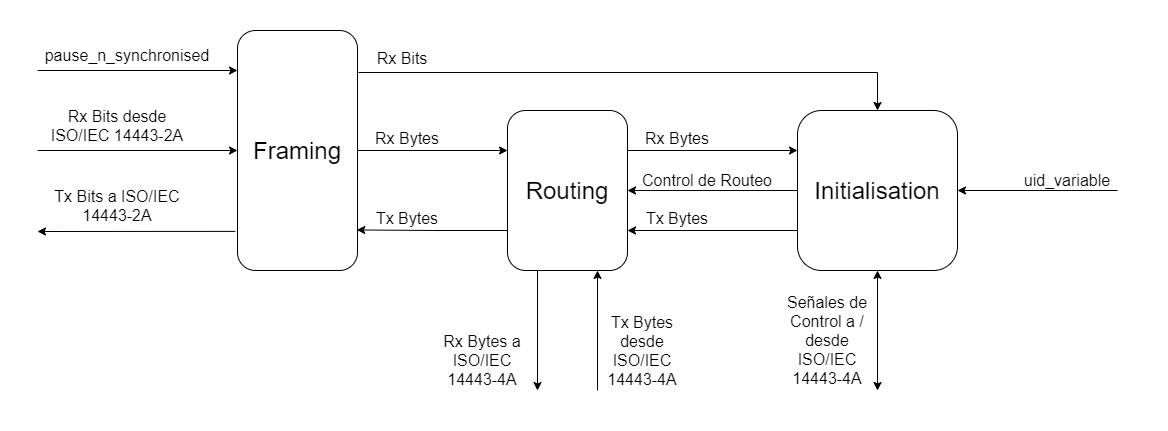
\includegraphics[width=0.95\textwidth]{./img/iso14443_3a.drawio}
  \caption{Diagrama en bloques del módulo \textbf{iso14443\_3a}.}
  \label{fig:iso14443_3a}
\end{figure}

Este módulo es parametrizado y los parámetros son descritos en el \tabref{tab:params_iso14443_3a}. Los parámetros del UID son pasados sin modificaciones al módulo \textbf{initialisation} y el parámetro \textit{FDT\_TIMING\_ADJUST} es pasado al módulo \textbf{framing}, también sin modificación.

\begin{table}[htb]
  \centering
  \tablezebra
  \begin{tabulary}{\linewidth}{l|l|L}
    \textbf{Nombre}&\textbf{Tipo}&\textbf{Descripción} \\
    \hline
    UID\_SIZE&UIDSize (enum)&La PICC tiene un UID simple, doble o triple. \\
    UID\_INPUT\_BITS&int&El ancho de la señal \textit{uid\_variable}. \\
    UID\_FIXED&logic [] (un vector)&Bits más significativos del UID. \\
    FDT\_TIMING\_ADJUST&int&Específica retardos en las rutas de recepción y transmisión externas a este módulo. \\
  \end{tabulary}
  \caption{Parámetros del módulo \textbf{iso14443\_3a}.}
  \label{tab:params_iso14443_3a}
\end{table}

\FloatBarrier

El banco de prueba para este módulo es muy parecido a lo del módulo \textbf{initialisation}. Las diferencias son:

\begin{itemize}
  \item No usa una \textbf{deserialiser}, ya que eso está incluido en el DUT.
  \item Usa un monitor \textbf{TxBitIfaceMonitor} en vez de \textbf{TxByteIfaceMonitor}, porque el DUT incluye el módulo \textbf{serialiser} que convierte las respuestas a bits.
  \item Tiene un monitor \textbf{RxByteIfaceMonitor} para la salida \textit{rx\_iface\_to\_14443\_4a}.
  \item Tiene un controlador \textbf{TxByteIfaceSourceDriver} para la entrada \textit{tx\_iface\_from\_14443\_4a}.
  \item El FDT es verificado de la misma manera que en el banco de prueba del módulo: \textbf{framing}.
  \item La clase \textbf{CommsTestsSequence} es extendida por \textbf{ISO14443\_3aTbSequence}, que incluye funcionalidades específicas por este banco de prueba. Mayormente las diferencias entre esta clase y la usada por el módulo \textbf{initialisation} son relacionadas con la verificación de las señales al módulo \textbf{iso14443\_4a}.
\end{itemize}

Como en el banco de prueba del módulo \textbf{initialisation}, este banco de prueba es ejecutado tres veces, una vez para cada tamaño de UID. El informe de cobertura por estas simulaciones dan resultados por el DUT de: 91\%, 92\% y 92\% por UIDs simples, dobles y triples respectivamente. Esos valores son para el DUT y sus submódulos. El DUT solo tiene 100\% cobertura en cada caso. Aunque unos de los submódulos faltan cobertura acá, todos tienen un porcentaje de cobertura alta en sus propios bancos de pruebas.

% ISO/IEC 14443-4A
\FloatBarrier
\subsection{ISO/IEC 14443-4A}

En este bloque de la implementación, solo hay un módulo \textbf{iso14443\_4a}, que es responsable para recibir, actuar sobre, y responder a las tramas definidas en la parte cuatro de la norma. Esas tramas son: RATS, PPS, y bloques estándares. El protocolo de nivel aplicación es encapsulado un campo de información en bloques estándares de tipo I. Ese campo es reenviado a la aplicación, y las respuestas de la aplicación son empaquetadas y enviadas hacia el PCD. Las salidas y entradas son descritas en el \tabref{tab:ports_iso14443_4a}.

\begin{table}[htb]
  \centering
  \tablezebra
  \begin{tabulary}{\linewidth}{l|l|L}
    \setcounter{rownum}{0}
    \textbf{Nombre}&\textbf{Dirección}&\textbf{Descripción} \\
    \hline
    clk&Entrada&Reloj. \\
    rst\_n&Entrada&Reset activo bajo. \\
    power&Entrada&Señal desde el AFE para indicar si la potencia recibida es apta. \\
    rx\_iface&Entrada&Sumidero para la \textit{rx\_interface}, conectado al módulo \textbf{iso14443\_3a}. \\
    rx\_crc\_ok&Entrada&La última trama recibida tiene CRC válido. \\
    tx\_iface&Salida&Fuente para la \textit{tx\_interface}, conectada al módulo \textbf{iso14443\_3a}. \\
    tx\_append\_crc&Salida&Indica que la respuesta debe tener CRC agregado. \\
    tag\_active&Entrada&La PICC está en el estado ACTIVE. \\
    rx\_rats&Salida&Indica que la trama RATS fue recibida. \\
    rx\_deselect&Salida&Indica que la trama S(DESELECT) fue recibida y la respuesta fue enviada. \\
    app\_rx\_iface&Salida&Fuente para la \textit{rx\_interface}, conectada a la aplicación. \\
    app\_tx\_iface&Entrada&Sumidero para la \textit{tx\_interface}, conectado a la aplicación. \\
    app\_resend\_last&Salida&La aplicación debe enviar su última respuesta de nuevo. \\
  \end{tabulary}
  \caption{Entradas y Salidas del módulo \textbf{iso14443\_4a}.}
  \label{tab:ports_iso14443_4a}
\end{table}

Cuándo una PICC recibe la trama SELECT con su UID, se transiciona al estado ACTIVE o ACTIVE*. En estos estados para terminar el proceso de inicialización el PCD envía una RATS. Cuando este módulo recibe esa trama mientras la entrada \textit{tag\_active} está en ‘1’, pulsa su salida \textit{rx\_rats}. El módulo \textbf{initialisation} usa esa señal para transicionar al estado PROTOCOL. La trama RATS contiene dos campos:

\begin{itemize}
  \item CID (Card Identifier): El PCD asigna un CID a la PICC para poder direccionar tramas a esta PICC si hay más de una inicializada. Este campo es cuatro bits, con el valor 15 reservado para uso futuro. El CID asignado es válido hasta que la PICC es desactivada.
  \item FSDI: Una codificación de 4 bits que representa el tamaño máximo de tramas que el PCD puede recibir. Este campo es ignorado porque todas las tramas usadas en este trabajo tienen tamaños menores que lo mínimo que los PCDs tienen que soportar.
\end{itemize}

La respuesta a RATS es ATS que consiste en al menos un byte, pero hay algunos campos de bytes opcionales. Estos bytes opcionales no son implementados en este trabajo, los argumentos presentes en estos bytes tienen valores por defectos adecuados para este trabajo.

Después de la RATS y ATS, el PCD opcionalmente puede enviar la trama PPS para cambiar las tasas de transmisión y recepción. El PCD solo es permitido enviar la PPS inmediatamente después de la recepción de la respuesta ATS, por lo tanto la PICC ignora tramas PPS en cualquier otro momento. Debido a que este trabajo no soporta otras tasas de bits, este módulo solo responde a la PPS si las tasas de bits especificadas son: $\nicefrac{f_c}{128}$ en cada dirección.

Un bloque estándar comienza con una cabecera de entre uno y tres bytes:

\begin{description}
  \item[PCB:] \hfill \\ Contiene: el tipo del bloque (I, R, o S), unos campos específicos del tipo de bloque, y dos indicadores que especifican si los campos de CID y NAD están presentes.
  \item[CID:] \hfill \\ Usado para direccionar una trama a una PICC en particular. Este campo en las tramas enviadas desde la PICC también contiene dos bits que indican si la PICC está recibiendo suficiente potencia desde el campo electromagnético. Estos bits son asignados al valor de la entrada \textit{power}, que es controlado por el AFE.
  \item[NAD (Node Address):] \hfill \\ Una PICC puede contener más de una aplicación y este campo permite el PCD direccionar tramas a una en particular. Este trabajo no soporta este campo, bloques estándares con una NAD son ignorados, como se especifica la norma.
\end{description}

Un objetivo de este trabajo es tomar muestras de múltiples de sensores discretos, así que es necesario tener más de una PICC activada a la vez, por lo tanto este diseño soporta CIDs. Una PICC que soporta el campo CID debe aceptar un bloque estándar que contiene su CID, y en el caso que su CID está 0, debe también aceptar bloques estándares que no contienen un CID. Otras tramas deben ser ignoradas~\cite{iso14443-4}. Este módulo incluye lógica combinatoria que determina si una trama es direccionada a esta PICC o no.

Bloques estándares de tipo I pueden contener un campo de información después de la cabecera. Esta información es un mensaje de nivel de aplicación. Cuándo este módulo recibe un bloque estándar tipo I, el campo de información es reenviado a la aplicación sobre la \textit{app\_rx\_iface}. La respuesta de la aplicación es recibida sobre la \textit{app\_tx\_iface}. Este módulo empaqueta la respuesta en un bloque estándar tipo I con los campos adecuados y envía la trama completa al PCD. Bloques estándares de tipo I pueden ser encadenados, esto permite el envío de tramas más grandes que el receptor soporta. La norma requiere que todos los PCDs y PICCs soporten tramas de al menos 16 bytes, y debido a que el protocolo de nivel aplicación de este trabajo solo usa tramas con tamaños menores que eso, bloques estándares encadenados no son soportados en esta implementación. Si este módulo recibe un bloque estándar tipo I encadenado, es ignorado.

Hay tres bloques estándares de tipo S definidos en la norma:

\begin{description}
  \item[S(DESELECT):] \hfill \\ La PICC debe transicionar al estado HALT. Este módulo pulsa la salida \textit{rx\_deselect} después de haber enviado la respuesta, que causa el módulo \textbf{initialisation} transicionar al estado HALT.
  \item[S(WTX):] \hfill \\ La PICC puede enviar esta respuesta a un bloque estándar tipo I si necesita más tiempo para procesar la solicitud. Este mensaje no es soportado en este trabajo debido a que todas las respuestas de nivel aplicación pueden ser calculado de forma inmediata.
  \item[S(PARAMETERS):] \hfill \\ El PCD puede usar este mensaje para cambiar la configuración de la PICC, por ejemplo para cambiar la tasa de bits. Este mensaje es opcional y no es soportado en esta implementación.
\end{description}

Bloques estándares de tipos I y R tienen un bit en el campo PCB que se llama el número de bloque. La PICC también tiene un registro de un bit que guarda un número de bloque. Cuándo la PICC envía un bloque estándar de tipo I o R, el número de bloque en la cabecera debe ser igual al valor en su registro. Las reglas de cómo manipular este registro en la PICC son:

\begin{displaycquote}[traducido de][]{iso14443-4}
  \begin{itemize}
    \item La PICC debe iniciar su número de bloque a ‘1’ cuando está activada.
    \item Cuando la PICC recibe un bloque estándar de tipo I, debe invertir el valor en su registro antes de enviar la respuesta.
    \item Cuando la PICC recibe un R(ACK) con número de bloque no igual a lo actual de la PICC, debe invertir el valor en su registro, antes de enviar la respuesta.
  \end{itemize}
\end{displaycquote}

Hay dos mensajes que usan bloques estándares de tipo R: R(ACK), y R(NAK). Las reglas de cómo la PICC debe responder a esos mensajes son:

\begin{displaycquote}[traducido de][]{iso14443-4}
  \begin{itemize}
    \item Cuando un R(ACK) o un R(NAK) es recibido, si el número de bloque [en la cabecera] es igual al número de bloque actual de la PICC, la PICC debe reenviar su última respuesta.
    \item Cuándo un R(NAK) es recibido, si el número de bloque [en la cabecera] no es igual al número de bloque actual de la PICC, la PICC debe responder con un R(ACK).
    \item Cuándo un R(ACK) es recibido, si el número de bloque [en la cabecera] no es igual al número de bloque actual de la PICC, y la última respuesta de la PICC fue encadenada, la PICC debe seguir con el siguiente bloque en la cadena.
  \end{itemize}
\end{displaycquote}

Este mecanismo es diseñado para facilitar el PCD recuperar después de la pérdida de una trama. Debido a que esta implementación no soporta bloques encadenados, solo las primeras dos reglas son implementadas, y los bloques R(ACK) son ignorados cuándo su número de bloque no es igual al valor guardado en la PICC. En el caso de recibir un R(ACK) o R(NAK) con el número de bloque igual al valor guardado en la PICC, la última respuesta es reenviada, y si la última respuesta fue un bloque estándar de tipo I, la salida \textit{app\_resend\_last} es pulsada para pedir la aplicación repetir su última respuesta también.

La ruta de recepción de tramas es parecida a la del módulo \textbf{initialisation}, la trama es guardada en un buffer. Después de la recepción de la cabecera, si este módulo determina que la trama es un bloque estándar tipo I direccionada a esta PICC, los bytes del campo de información son reenviados a la aplicación. El buffer de recepción tiene cinco bytes para poder guardar la trama de tamaño máximo: PPS. Aunque bloques estándares de tipo I pueden ser más largos, este módulo solo guarda los primeros dos bytes de la cabecera: PCB y CID.

La ruta de transmisión también es parecida a la del módulo \textbf{initialisation}. Un buffer de dos bytes es usado para construir las respuestas. Cuando una respuesta está lista para enviar, la salida \textit{tx\_iface.data\_valid} es fijada en ‘1’, y el primer byte de la respuesta es asignado a la salida \textit{tx\_iface.data}. Cuando el sumidero pide el próximo byte mediante la señal \textit{tx\_iface.req}, la salida \textit{tx\_iface.data} es actualizada con el próximo byte. En el caso de que la respuesta sea un bloque estándar tipo I, el buffer es llenado con la cabecera correspondiente. Después del envío de la cabecera este módulo actúa como un pass-through por la respuesta de la aplicación. Debido a que las respuestas: ATS, PPS y todos los bloques estándares tienen un CRC, la salida \textit{tx\_append\_crc} es un ‘1’ constante.

El banco de prueba para este módulo es parecido a los bancos de pruebas de los módulos \textbf{initialisation} y \textbf{iso14443\_3a}, pero ejecuta pruebas distintas que son diseñadas para verificar la parte cuatro de la norma. El banco de prueba incluye la clase \textbf{ISO14443\_4a\-TbSequence} que extiende \textbf{CommsTestSequence} para proveer funcionalidades específicas a este banco de prueba:

\begin{itemize}
  \item Verifica que los campos de información de bloques estándares de tipos I son reenviados a la aplicación, y que otras tramas no son reenviadas a la aplicación.
  \item Maneja las entradas \textit{rx\_crc\_ok}, \textit{power} y \textit{tag\_active} del DUT y verifica el comportamiento de sus salidas: \textit{rx\_rats}, \textit{rx\_deselect}, y \textit{rx\_app\_resend\_last}.
  \item Simula respuestas desde la aplicación.
  \item Sustituye las tareas \textbf{go\_to\_state\_*()}. La secuencia usa estas tareas para poner el DUT en el estado apto para cada prueba, pero en este caso el DUT no contiene la máquina de estados de la parte tres de la norma, por lo tanto las transiciones entre estos estados tienen que ser simuladas.
\end{itemize}

La parte cuatro de la norma especifica algunas reglas sobre el comportamiento de una PICC, las pruebas en este banco de prueba verifican que esas reglas se cumplen, entre otras cuestiones. Las pruebas ejecutadas son en la tarea \textbf{run\_all\_part4\_tests()} de la clase \textbf{CommsTestSequence}. Unos ejemplos de las pruebas son:

\begin{itemize}
  \item Verifica que cuando una PICC en el estado ACTIVE o ACTIVE* recibe una trama RATS con CID válido, envía la respuesta ATS esperada, y si la PICC es en otro estado o el CID asignado no es válido, la PICC no envía una respuesta.
  \item Verifica que el DUT solo responde a la trama PPS cuándo es la primera trama después del envío de la respuesta ATS.
  \item Verifica que cuando la PICC está en el estado PROTOCOL, los campos de información en los bloques estándares de tipo I, son enviados a la aplicación.
  \item Verifica que el DUT cumple con las reglas descritas arriba sobre los números de bloques.
\end{itemize}

El informe de cobertura da el DUT un resultado de 98\%. Las partes que faltan cobertura son situaciones imposibles de ocurrir, por ejemplo: la salida \textit{tx\_append\_crc} es un ‘1’ constante, por lo tanto falta cobertura de toggle.

% ISO/IEC 14443A
\FloatBarrier
\subsection{ISO/IEC 14443A}

Este módulo es el módulo más alto del núcleo IP. Debería ser instanciado en la aplicación y conectado a un AFE conforme con parte dos de la norma. El módulo simplemente instancia los módulos: \textbf{iso14443\_2a}, \textbf{iso14443\_3a}, \textbf{iso14443\_4a}, y los conecta de forma adecuada. Este módulo es parametrizado y los parámetros son descritos en el \tabref{tab:params_iso14443a}. Las salidas y entradas son descritas en el \tabref{tab:ports_iso14443a}.

\begin{table}[htb]
  \centering
  \tablezebra
  \begin{tabulary}{\linewidth}{l|l|L}
    \textbf{Nombre}&\textbf{Tipo}&\textbf{Descripción} \\
    \hline
    UID\_SIZE&UIDSize (enum)&La PICC tiene un UID simple, doble o triple. \\
    UID\_INPUT\_BITS&int&El ancho de la señal \textit{uid\_variable}. \\
    UID\_FIXED&logic [] (un vector)&Bits más significativos del UID. \\
    FDT\_TIMING\_ADJUST&int&Específica retardos en la ruta de recepción y transmisión externa a este módulo. \\
  \end{tabulary}
  \caption{Parámetros del módulo \textbf{iso14443a}.}
  \label{tab:params_iso14443a}
\end{table}

Los parámetros del UID son igual a los definidos en el módulo \textbf{iso14443\_3a}, y son pasados a ese módulo sin modificaciones. El parámetro \textit{FDT\_TIMING\_ADJUST} es usado para ajustar el comportamiento del módulo \textbf{FDT} para que cumpla con el FDT especificado en la norma. El módulo \textbf{iso14443\_2a} contiene tres ciclos de retardo en el envío de las respuestas. Por lo tanto, el módulo \textbf{iso14443\_3a} es instanciado con su parámetro \textit{FDT\_TIMING\_ADJUST} igual al valor del parámetro en este módulo más tres.

El banco de prueba para este módulo está basado en una mezcla de los bancos de pruebas de los módulos \textbf{iso14443\_3a} y \textbf{iso14443\_4a}. Este banco de prueba usa el modelo del AFE para generar el reloj y las pausas. El FDT es verificado, midiendo el tiempo entre el último flanco ascendente de la señal \textit{pause\_n\_synchronised} y el primer flanco ascendente de la señal \textit{lm\_out}. Las pruebas ejecutadas son las pruebas de inicialización y las de la parte cuatro de la norma. Esas pruebas son repetidas diez veces con la parte variable del UID diferente cada vez.

\begin{table}[htb]
  \centering
  \tablezebra
  \begin{tabulary}{\linewidth}{l|l|L}
    \textbf{Nombre}&\textbf{Dirección}&\textbf{Descripción} \\
    \hline
    clk&Entrada&Reloj. \\
    rst\_n&Entrada&Reset, activo bajo. El flanco ascendente debe ser sincronizado al reloj. \\
    uid\_variable&Entrada&Bits menos significativos del UID. \\
    power&Entrada&Señal desde el AFE que indica si la potencia recibida es apta. \\
    pause\_n\_synchronised&Entrada&Pausa, activa baja, sincronizada. \\
    lm\_out&Salida&Salida al modulador de carga para enviar respuestas. \\
    app\_rx\_iface&Salida&Fuente para la \textit{rx\_interface}, conectada a la aplicación. \\
    app\_tx\_iface&Entrada&Sumidero para la \textit{tx\_interface}, conectada a la aplicación. \\
    app\_resend\_last&Salida&Un indicador para pedir la aplicación reenviar su última respuesta. \\
    iso14443a\_version&Salida&La versión de este núcleo IP, debe ser constante. \\
  \end{tabulary}
  \caption{Entradas y Salidas del módulo \textbf{iso14443a}.}
  \label{tab:ports_iso14443a}
\end{table}

Como por el banco de prueba del módulo \textbf{initialisation}, este banco de prueba es ejecutado tres veces, una vez para cada tamaño del UID. El informe de cobertura por estas tres simulaciones dan resultados por el DUT de: 92\%, 93\% y 93\% por UIDs simples, dobles y triples respectivamente. Esos resultados son por el DUT y sus submódulos. El DUT solo, tiene 89\%, 93\% y 95\% cobertura en cada caso. Las partes que faltan cobertura son porque la salida \textit{iso14443a\_version} y la señal interna \textit{part4\_tx\_append\_crc} son constantes. Aunque algunos de los submódulos no poseen alta cobertura en esta prueba, todos tienen un alto porcentaje de cobertura en sus propios bancos de pruebas.

% Otros
\FloatBarrier
\subsection{Otros}

Hay algunos módulos extras que no son usados en este núcleo IP, son incluidos para uso en la aplicación si son necesarios.

% synchroniser
\FloatBarrier
\subsubsection{synchroniser}

Este módulo sincroniza una señal al dominio del reloj para prevenir metaestabilidad~\cite{synch_arb_in_digital_systems}. Este módulo es parametrizado y sus parámetros se describen en el \tabref{tab:params_synchroniser}. Las salidas y entradas son descritas en el \tabref{tab:ports_synchroniser}. La implementación es dos registros conectados como se muestra la \figref{fig:synchroniser}.

\begin{table}[htb]
  \centering
  \tablezebra
  \begin{tabulary}{\linewidth}{l|l|L}
    \textbf{Nombre}&\textbf{Tipo}&\textbf{Descripción} \\
    \hline
    WIDTH&int&Ancho de la señal a sincronizar. \\
    RESET\_VAL&logic [WIDTH-1:0]&Valor de la salida cuándo el módulo está en un estado de reset. \\
  \end{tabulary}
  \caption{Parámetros del módulo \textbf{synchroniser}.}
  \label{tab:params_synchroniser}
\end{table}

\begin{table}[htb]
  \centering
  \tablezebra
  \begin{tabulary}{\linewidth}{l|l|L}
    \textbf{Nombre}&\textbf{Dirección}&\textbf{Descripción} \\
    \hline
    clk&Entrada&Reloj. \\
    rst\_n&Entrada&Reset activo bajo. \\
    D&Entrada&Señal a sincronizar. \\
    Q&Salida&Señal sincronizada. \\
  \end{tabulary}
  \caption{Entradas y Salidas del módulo \textbf{synchroniser}.}
  \label{tab:ports_synchroniser}
\end{table}

\begin{figure}[htb]
  \centering
  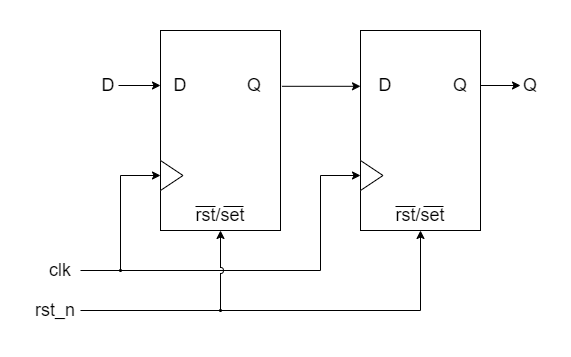
\includegraphics[width=0.6\textwidth]{./img/synchroniser.drawio}
  \caption{El circuito implementado en el módulo \textbf{synchroniser}.}
  \label{fig:synchroniser}
\end{figure}

Debido a la simplicidad de este módulo no hay un banco de prueba, el comportamiento debería ser verificado en los bancos de prueba de los módulos que lo usan.

% active_low_reset_synchroniser
\FloatBarrier
\subsubsection{active\_low\_reset\_synchroniser}

Este módulo es un sincronizador de reset para sincronizar el flanco ascendente de resets asincrónicos, activos bajos, para prevenir metaestabilidad cuándo el diseño sale del estado de reset. Las salidas y entradas se describe en el \tabref{tab:ports_active_low_reset_synchroniser}. La implementación simplemente es dos registros como se muestra la \figref{fig:active_low_reset_synchroniser}. Como en el caso del módulo synchroniser, no hay banco de prueba para este módulo.

\begin{table}[htb]
  \centering
  \tablezebra
  \begin{tabulary}{\linewidth}{l|l|L}
    \setcounter{rownum}{0}
    \textbf{Nombre}&\textbf{Dirección}&\textbf{Descripción} \\
    \hline
    clk&Entrada&Reloj. \\
    rst\_n\_in&Entrada&Reset a sincronizar, activo bajo. \\
    rst\_n\_out&Salida&Reset con su flanco ascendente sincronizado, activo bajo. \\
  \end{tabulary}
  \caption{Entradas y Salidas del módulo \textbf{active\_low\_reset\_synchroniser}.}
  \label{tab:ports_active_low_reset_synchroniser}
\end{table}

\begin{figure}[htb]
  \centering
  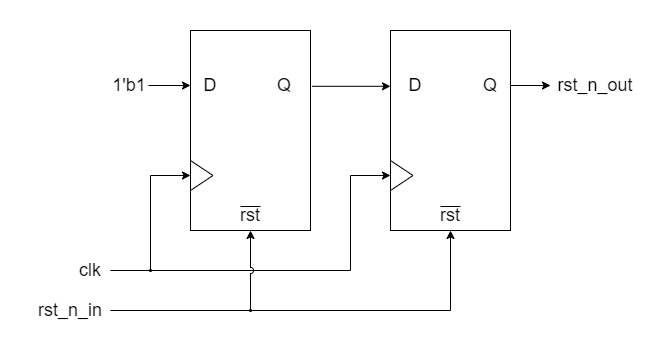
\includegraphics[width=0.8\textwidth]{./img/active_low_reset_synchroniser.drawio}
  \caption{El circuito implementado en el módulo \textbf{active\_low\_reset\_synchroniser}.}
  \label{fig:active_low_reset_synchroniser}
\end{figure}

% pause_n_latch_and_synchroniser
\FloatBarrier
\subsubsection{pause\_n\_latch\_and\_synchroniser}

En el caso de un AFE que produce un reloj que se detiene durante las pausas, si no se puede garantizar que haría al menos un flanco ascendente del reloj mientras la pausa está activa, sería necesario usar un circuito asincrónico para retener las pausas hasta que el reloj comience de nuevo. El circuito usado es un FFD (Flip Flop D) con un reset y un set asincrónicos, conectado como se muestra en la \figref{fig:pause_n_latch}. La entrada \textit{pause\_n\_async} es conectada a la reset asincrónica, así durante la pausa, la salida \textit{pause\_n\_latched} es ‘0’. La entrada D del FFD es un ‘1’ constante, así en el primer flanco ascendente del reloj después de la pausa, la salida \textit{pause\_n\_latched} vuelve a ‘1’. La entrada \textit{rst\_n} está conectada a la set asincrónica, así durante un reset la salida es ‘1’. Debido a que se usa un reset asincrónico el flanco descendente de la  \textit{pause\_n\_latched} es asincrónica al reloj, por lo tanto es necesario usar un sincronizador para prevenir metaestabilidad. La \figref{fig:pause_n_synch_and_latch} muestra el diseño final.

\begin{figure}[htb]
  \centering
  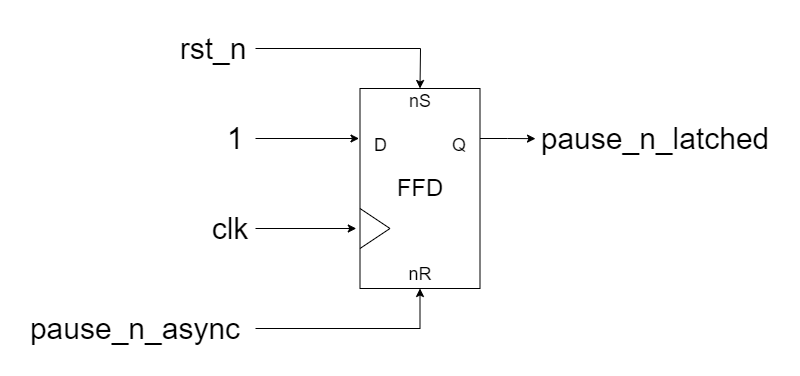
\includegraphics[width=0.6\textwidth]{./img/pause_latch_and_synch1_latching.drawio}
  \caption{Circuito asincrónico por la retención de pausas.}
  \label{fig:pause_n_latch}
\end{figure}

\begin{figure}[htb]
  \centering
  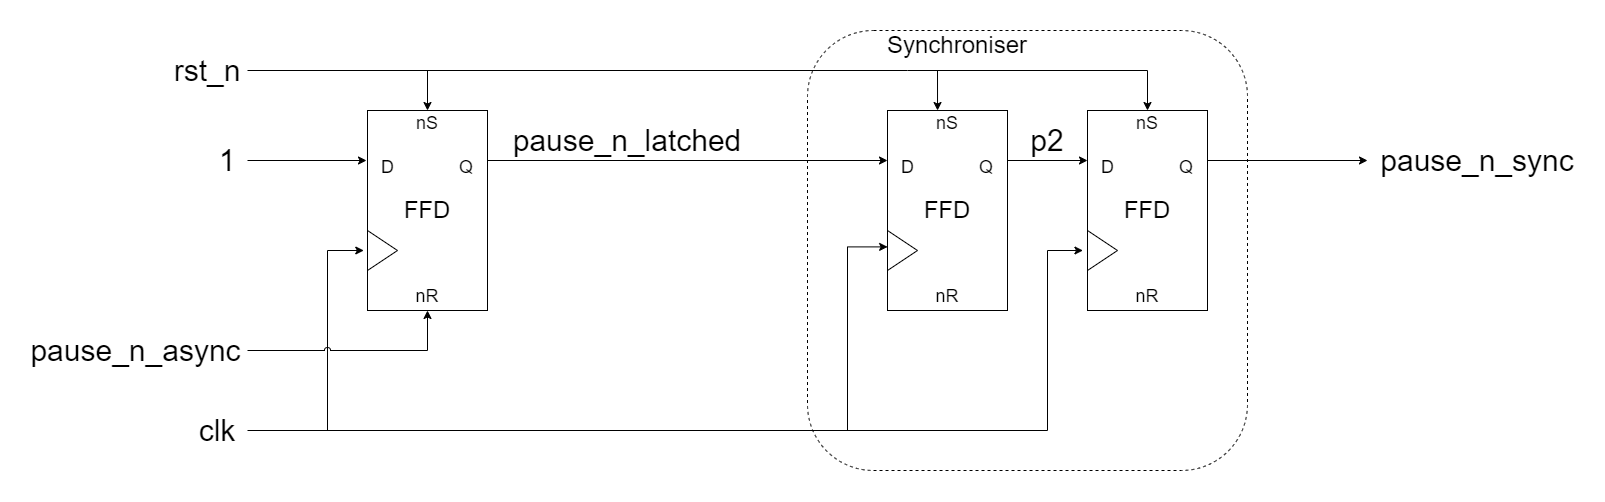
\includegraphics[width=1.0\textwidth]{./img/pause_latch_and_synch1_ffd.drawio}
  \caption{\small{El circuito implementado en el módulo \textbf{pause\_n\_latch\_and\_synchroniser}.}}
  \label{fig:pause_n_synch_and_latch}
\end{figure}

\FloatBarrier

Las salidas y entradas son descritas en el \tabref{tab:ports_pause_n_synch_and_latch}. La \figref{fig:pause_n_synch_and_latch_timing} muestra un diagrama de timing de este diseño cuándo el reloj está detenido durante la pausa entera.

\begin{table}[htb]
  \centering
  \tablezebra
  \begin{tabulary}{\linewidth}{l|l|L}
    \textbf{Nombre}&\textbf{Dirección}&\textbf{Descripción} \\
    \hline
    clk&Entrada&Reloj. \\
    rst\_n&Entrada&Reset activo bajo. \\
    pause\_n\_async&Entrada&Pausa, asincrónica, desde el AFE. \\
    pause\_n\_sync&Salida &Pausa retenida y sincronizada. \\
  \end{tabulary}
  \caption{Entradas y Salidas del módulo \textbf{pause\_n\_synch\_and\_latch}.}
  \label{tab:ports_pause_n_synch_and_latch}
\end{table}

\begin{figure}[htb]
  \centering
  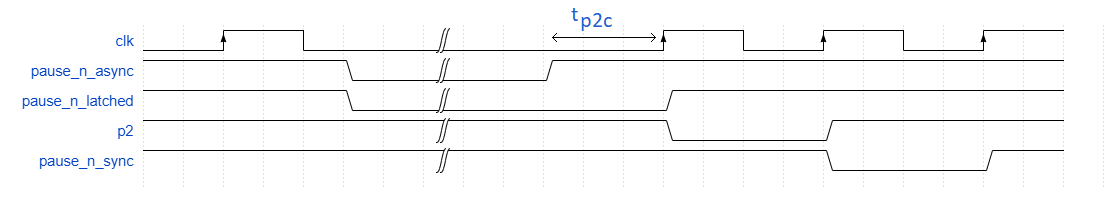
\includegraphics[width=1.0\textwidth]{./img/pause_latch_sync_dff_timing_1}
  \caption{Diagrama de timing de una pausa sin reloj.}
  \label{fig:pause_n_synch_and_latch_timing}
\end{figure}

Para cumplir con el FDT definida en la parte tres de la norma es necesario compensar por el retardo entre los flancos ascendentes de las señales \textit{pause\_n\_async} y \textit{pause\_n\_sync}. Este retardo es dos ciclos del reloj más $t_{p2c}$. En este trabajo el mecanismo para compensar por este retardo es con el parámetro \textit{FDT\_TIMING\_ADJUST} del módulo más alto del núcleo IP. Cualquier diseño que instancia este núcleo IP y usa este módulo para retener y sincronizar las pausas debe incluir estos retardos en la calculación del parámetro \textit{FDT\_TIMING\_ADJUST}.

Para verificar este módulo el modelo analógico: \textbf{analogue\_sim} es usado para enviar miles de pausas con la relación entre la señal \textit{pause\_n\_async} y el reloj elegido aleatoriamente por cada pausa. Unas aserciones son usadas para verificar los retardos entre la entrada y la salida. El informe de cobertura da un resultado de 100\% por el DUT.

% Aplicación - Interfaz con el sensor MOSFET de radiación y el ADC
% --------------------------------
\FloatBarrier
\section{Aplicación - Interfaz con el sensor y ADC}

La aplicación es el bloque principal de este trabajo, instancia el núcleo IP ISO/IEC 14443A, recibe, actúa sobre, y responde a los mensajes de nivel aplicación contenidos en bloques estándares de tipo I. El propósito de este bloque es proveer un método para manipular las salidas al sensor y al ADC, y para devolver la muestra al PCD. El \tabref{tab:sens_adc_signals} muestra las señales conectadas al sensor y al ADC:

\begin{table}[htb]
  \centering
  \tablezebra
  \begin{tabulary}{\linewidth}{l|l|L}
    \setcounter{rownum}{0}
    \textbf{Nombre}&\textbf{Dirección}&\textbf{Descripción} \\
    \hline
    sens\_config[2:0]&Salida&Configuración del sensor. \\
    sens\_enable&Salida&Activa el sensor. \\
    sens\_read&Salida&Lee el sensor. \\
    sens\_version[3:0]&Entrada&Versión del sensor. \\
    adc\_enable&Salida&Activa el ADC. \\
    adc\_read&Salida&Lee el ADC. \\
    adc\_conversion\_complete&Entrada&Indica que el ADC ha tomado la muestra. \\
    adc\_value[15:0]&Entrada&Dato muestreado. \\
    adc\_version[3:0]&Entrada&Versión del ADC. \\
  \end{tabulary}
  \caption{Señales en la interfaz con el sensor y el ADC.}
  \label{tab:sens_adc_signals}
\end{table}

La \figref{fig:sens_adc} muestra el proceso para tomar una muestra del sensor. Primero se fija \textit{sens\_config} con el valor deseado para elegir la configuración del sensor. Después las señales \textit{sens\_enable} y \textit{adc\_enable} son asignadas el valor ‘1’ para activar los dos componentes. Después de un tiempo ($t_1$) la señal \textit{sens\_read} debe ser asignado con el valor ‘1’ para pedir que el sensor comienza una lectura. Siguiente, después de un tiempo ($t_2$) la señal \textit{adc\_read} debe ser asignado con el valor ‘1’ para pedir que el ADC comience a tomar una muestra. Cuándo el ADC termina la lectura debe pulsar la señal \textit{adc\_conversion\_complete} por un ciclo del reloj para indicar que la señal \textit{adc\_value} es válida y estable. La interpretación de estas señales está a cargo del diseñador del sensor y del ADC, siendo que está fuera del alcance de este trabajo. El valor de \textit{sens\_config} y los valores de $t_1$ y $t_2$ pueden ser controlados por el PCD al tiempo de la lectura.

\begin{figure}[htb]
  \centering
  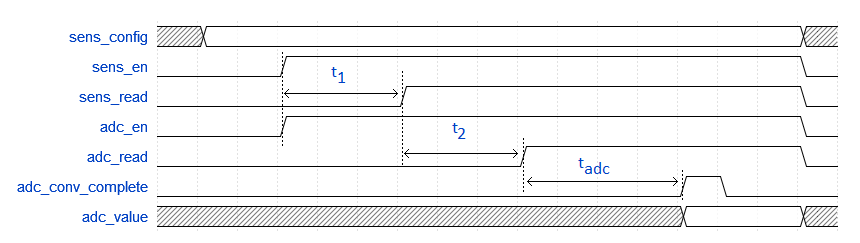
\includegraphics[width=0.9\textwidth]{./img/sens_adc}
  \caption{Diagrama de timing de una lectura del sensor.}
  \label{fig:sens_adc}
\end{figure}

% Sincronización del muestreo
\FloatBarrier
\subsection{Sincronización del muestreo}

Para cumplir con las metas del proyecto marco es requerido poder tomar muestras de múltiples de TAGs de forma sincronizada. Un método para sincronizar las muestras sería usar una trama broadcast para iniciar el proceso en cada PICC a la vez. Desafortunadamente la norma ISO/IEC 14443-4 no permite al PCD envíar bloques estándares de forma broadcast. Sería posible modificar el diseño del núcleo IP para permitir esto, por ejemplo con el CID 15 que es reservado para uso futuro en la norma. La desventaja de esto es que no conforme con la norma y significaría que el núcleo IP no sería una implementación genérica.

El método usado para sincronizar las muestras en este trabajo es parecido a como el FDT funciona para sincronizar las respuestas de las tramas de ANTICOLLISION. Todas las PICCs reciben las pausas mediante el mismo circuito, por lo tanto el flanco ascendente de la pausa debe ser recibido en todas las PICCs a aproximadamente el mismo momento. Además las PICCs recuperan sus relojes de la portadora, así todas las PICCs en el campo electromagnético de un PCD tienen relojes con exactamente la misma frecuencia. Estos hechos significan que si las PICCs tienen un contador que es reseteado a cero en cada flanco ascendente de la pausa, y en los otros ciclos del reloj incrementa su valor, los contadores estarían sincronizados dentro de un margen de error de unos ciclos del reloj. El margen de error exacto depende en la implementación del AFE.

Unos de los mensajes en el protocolo propietario diseñado por este trabajo tienen un campo de sincronización. Una PICC que recibe uno de esos mensajes no realiza la acción especificada hasta que su contador de sincronización ha llegado al valor especificado en ese campo. El PCD puede enviar el mismo mensaje a cada PICC activa en turno. Con un tiempo de sincronización suficientemente grande el PCD puede enviar la siguiente trama antes de que la acción sea realizada, reseteando los contadores en todas las PICCs. De esta manera se logra que todas las PICCs realizan la misma acción de forma sincronizada.

El tiempo de sincronización tiene que ser más grande que el tiempo entre el flanco ascendente de la última pausa de una trama enviada por el PCD y el flanco ascendente de la primera pausa en la próxima trama: $t_{synch} > t_{fdt1} + t_{respuesta} + t_{fdt2} + t_p$ como se muestra la \figref{fig:app_synch}. Los valores en ciclos del reloj son:

\begin{description}[font=\normalfont]
  \item[$t_{fdt1} = 1236$ ciclos:] \hfill \\ El FDT máximo entre el último flanco ascendente de una trama desde el PCD y el primer flanco de modulación de la respuesta, como definida en la norma~\cite{iso14443-3}.
  \item[$t_{respuesta} = 128 \left(B + 1\right)$ ciclos:] \hfill \\ El tiempo necesario para enviar la respuesta, dónde B es el máximo número de bits en la respuesta incluyendo la cabecera, el CRC y los bits de paridad. En el protocolo la respuesta más grande a un comando con sincronización es diez bytes, por lo tanto $B = \SI{90}{bits}$, y $t_{respuesta} = \SI{11648}{ciclos}$.
  \item[$t_{fdt2} = 1272$ ciclos:] \hfill \\ El FDT entre el último flanco de modulación en una respuesta y el primer flanco de la pausa de la próxima trama del PCD, como definida en la norma~\cite{iso14443-3}. Este valor es el mínimo requerido por la norma, el valor actual depende en la implementación del PCD.
  \item[$t_p \approx 32$ ciclos:] \hfill \\ La duración de una pausa.
\end{description}

Estos valores dan un resultado de $t_{sync} > \SI{14188}{ciclos}$ ($t_{sync} > \SI{1.0}{\milli\second}$).

\begin{figure}[htb]
  \centering
  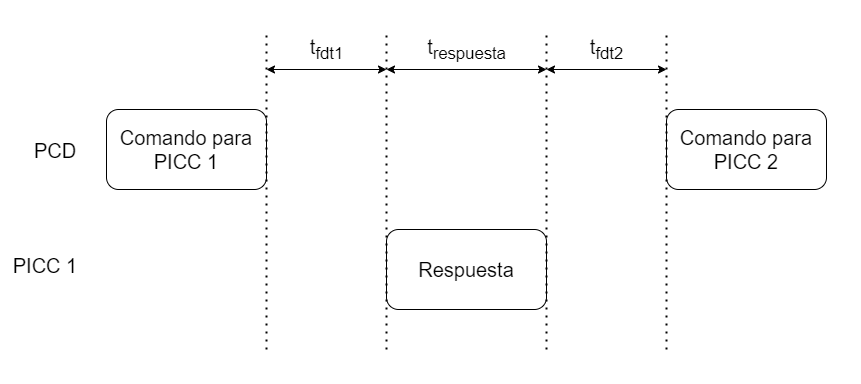
\includegraphics[width=0.7\textwidth]{./img/app_synch3.drawio}
  \caption{Timings para sincronizar acciones en más de una PICC.}
  \label{fig:app_synch}
\end{figure}

% Protocolo Propietario
\FloatBarrier
\subsection{Protocolo Propietario}

El protocolo de nivel aplicación es un protocolo propietario diseñado para este trabajo, el \appref{appendix:protocol_defs} contiene un header del lenguaje de programación C con definiciones y estructuras por este protocolo. Cada mensaje y respuesta comienzan con una cabecera de cinco bytes que consiste en un valor mágico de cuatro bytes, y un byte para indicar el tipo de comando. El valor mágico está presente porque la norma ISO/IEC 14443 no define un método para determinar qué protocolo de aplicación usa una PICC. Al comenzar cada mensaje y respuesta con un valor mágico provee un método para verificar que un PCD y una PICC son compatibles. Los comandos definidos son:

\begin{description}
  \item[IDENTIFY:] \hfill \\ Solicitud por las versiones de los bloques. El PCD puede usar la respuesta para determinar qué revisión de silicio usa una PICC. No lleva argumentos.
  \item[SET\_SIGNAL:] \hfill \\ Solicitud para cambiar las señales al sensor y al ADC. Esta acción puede ser sincronizada con otras PICCs. Lleva tres argumentos:
  \begin{itemize}
    \item \textit{sync[15:0]}: Tiempo de sincronización.
    \item \textit{mask[7:0]}: Máscara de bits para especificar qué señales cambiar. Los bits son:
    \begin{tabular}{r l}
      7-5: & \textit{sens\_config[2:0]} \\
      4: & \textit{sens\_enable} \\
      3: & \textit{sens\_read} \\
      2: & \textit{adc\_enable} \\
      1: & \textit{adc\_read} \\
      0: & reservado \\
    \end{tabular}
    %\begin{description}[labelwidth=2cm]
    %  \item[7-5:] \textit{sens\_config[2:0]} \\
    %  \item[4:] \textit{sens\_enable} \\
    %  \item[3:] \textit{sens\_read} \\
    %  \item[2:] \textit{adc\_enable} \\
    %  \item[1:] \textit{adc\_read} \\
    %  \item[0:] reservado \\
    %\end{description}
    \item \textit{value}: Valores nuevos de esas señales.
  \end{itemize}
  \item[AUTO\_READ:] \hfill \\ Solicitud para tomar una muestra del sensor automáticamente. Esta acción puede ser sincronizada con otras PICCs. Lleva tres argumentos, los argumentos \textit{timing1} y \textit{timing2} corresponden con el $t_1$ y $t_2$ mostrados en la \figref{fig:sens_adc}:
  \begin{itemize}
    \item \textit{sync[15:0]}: Tiempo de sincronización.
    \item \textit{timing1[31:0]}: Tiempo entre los flancos ascendentes de las señales \textit{sens\_enable} y \textit{adc\_enable}, y el flanco ascendente de la señal \textit{sens\_read}. El protocolo usa 32 bits para este argumento, pero solo los 25 bits menos significativos son usados.
    \item \textit{timing2[31:0]}: Tiempo entre el flanco ascendente de la señal \textit{sens\_read} y el flanco ascendente de la señal \textit{adc\_read}. El protocolo usa 32 bits para este argumento, pero solo los 25 bits menos significativos son usados.
  \end{itemize}
  \item[GET\_RESULT:] \hfill \\ Solicitud por el valor de la última muestra. No lleva argumentos.
  \item[ABORT:] \hfill \\ Solicitud para abandonar la acción concurrente, sea una AUTO\_READ o una SET\_SIGNAL. No lleva argumentos.
\end{description}

Las respuestas son:

\begin{description}
  \item [IDENTIFY\_REPLY:] \hfill \\ Respuesta al IDENTIFY, contiene:
  \begin{itemize}
    \item Versión de este protocolo.
    \item Versión de esta aplicación.
    \item Versión del núcleo IP ISO/IEC 14443A.
    \item Versión del sensor MOSFET de radiación.
    \item Versión del ADC.
  \end{itemize}
  \item [GET\_RESULT\_REPLY:] \hfill \\ Respuesta al GET\_RESULT, contiene el valor de la última muestra del sensor, y unas flags de estado:
  \begin{itemize}
    \item \textit{conv\_complete}: Indica que el ADC ha terminado una muestra después de la última vez que este flag fue enviado.
    \item \textit{already\_busy}: Indica que la PICC sigue ocupada, y no puede procesar esta solicitud.
    \item \textit{unexpected\_pause}: Indica que una pausa fue recibida durante los periodos de $t_1$, $t_2$, o $t_{adc}$ del proceso AUTO\_READ. Durante esos periodos el PCD debe quedarse quieto para que la PICC pueda tener un reloj continuo para medir los timings de forma precisa.
    \item \textit{error}: Indica que el último mensaje contuvo un error del protocolo, por ejemplo el comando no fue conocido, o el mágico fue inválido.
  \end{itemize}
  \item [STATUS\_REPLY:] \hfill \\ Respuesta a SET\_SIGNAL, AUTO\_READ y ABORT, contiene los mismos flags de estado de la respuesta GET\_RESULT\_REPLY.
\end{description}

% Ejemplos
\FloatBarrier
\subsection{Ejemplos}

Un ejemplo de la lectura de un único sensor mediante el comando SET\_SIGNAL. En este proceso los timings entre las etapas son controlados completamente por cuándo el PCD envía las tramas. El argumento \textit{sync} en todos casos debería ser cero.

\begin{enumerate}
  \item El PCD activa la PICC.
  \item El PCD envía el comando IDENTIFY y verifica la respuesta.
  \item El PCD envía el comando SET\_SIGNAL para fijar la señal \textit{sens\_config} como desea y las otras señales en ‘0’.
  \item El PCD envía el comando SET\_SIGNAL para fijar las señales \textit{sens\_enable} y \textit{adc\_enable} en ‘1’.
  \item El PCD espera por el $t_1$ deseado.
  \item El PCD envía el comando SET\_SIGNAL para fijar la señal \textit{sens\_read} en ‘1’.
  \item El PCD espera por el $t_2$ deseado.
  \item El PCD envía el comando SET\_SIGNAL para fijar la señal \textit{adc\_read} en ‘1’.
  \item El PCD espera por el $t_{adc}$, que depende en la implementación del ADC.
  \item El PCD envía el comando GET\_RESULT, verifica que la respuesta no indica un error, y guarda la muestra.
\end{enumerate}

Un ejemplo de la lectura de un único sensor mediante el comando AUTO\_READ. El argumento \textit{sync} en todos casos debería ser cero.

\begin{enumerate}
  \item El PCD activa la PICC.
  \item El PCD envía el comando IDENTIFY y verifica la respuesta.
  \item El PCD envía el comando SET\_SIGNAL para fijar la señal \textit{sens\_config} como desea y las otras señales en ‘0’.
  \item El PCD envía el comando AUTO\_READ, con los tiempos $t_1$ y $t_2$ deseados, y verifica la respuesta.
  \item El PCD espera por más que $t_1 + t_2 + t_{adc}$ para que el proceso se termine.
  \item El PCD envía el comando GET\_RESULT, verifica que la respuesta no indica un error, y guarda la muestra.
\end{enumerate}

Un ejemplo de la lectura de dos sensores de forma sincronizada mediante el comando AUTO\_READ. La \figref{fig:app_flow} muestra el mismo flujo de forma gráfica.

\begin{enumerate}
  \item El PCD activa las dos PICCs.
  \item El PCD envía el comando IDENTIFY a PICC 1 y PICC 2 por turnos, y verifica las respuestas.
  \item El PCD envía el comando SET\_SIGNAL a PICC 1 y PICC 2 por turnos, para fijar las señales \textit{sens\_config} como desea, y las otras señales en ‘0’. El argumento \textit{sync} debería ser cero, siendo que este comando no necesita ser sincronizado.
  \item El PCD envía el comando AUTO\_READ a PICC 1 y PICC 2 por turnos, especificando los mismos  $t_{sync}$, $t_1$ y $t_2$, en los dos mensajes.
  \item El PCD espera más que $t_{sync} + t_1 + t_2 + t_{adc}$ para que los procesos terminen.
  \item El PCD envía el comando GET\_RESULT a PICC 1 y PICC 2 por turnos, verifica las respuestas no indicas errores, y guarda las muestras.
\end{enumerate}

\begin{figure}[htb]
  \centering
  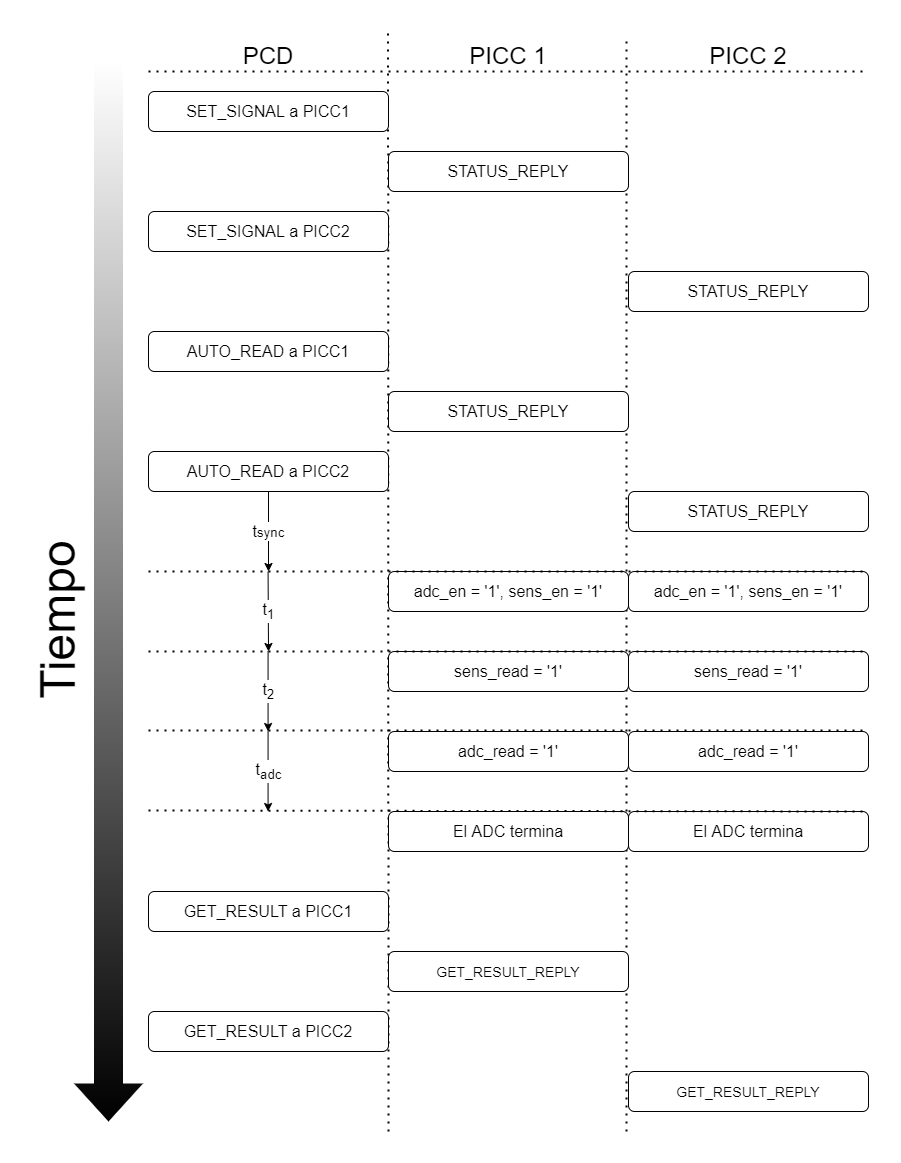
\includegraphics[width=1.0\textwidth]{./img/app_flow2.drawio}
  \caption{Ejemplo de la lectura de dos TAGs de forma sincronizada.}
  \label{fig:app_flow}
\end{figure}


% Marco de Verificación Extendido
\FloatBarrier
\subsection{Marco de Verificación Extendido}

El Marco de Verificación usado en el núcleo IP ISO/IEC 14443A es extendido para permitir la verificación de esta aplicación. Tres componentes extras son agregados.

\begin{itemize}
  \item Un paquete de SystemVerilog \textbf{ProtocolGenerator} que tienen funciones para generar colas de bytes por los mensajes de nivel aplicación.
  \item Una secuencia \textbf{AppCommsTestSequence} que extiende \textbf{CommsTestSequence}. Esta secuencia contiene unas pruebas adicionales para verificar el comportamiento de la aplicación. Estas pruebas son descritas dónde son usadas primero.
  \item Un modelo del ADC. Este modelo monitorea la señal \textit{adc\_read} por flancos ascendentes. Un número de ciclos después de la activación de esa señal, fija la señal \textit{adc\_value} en un valor aleatorio, y pulsa la señal \textit{adc\_conversion\_complete} por un ciclo. El retardo es elegido aleatoriamente entre un mínimo y un máximo que son parámetros del modelo.
\end{itemize}

% Implementación
\FloatBarrier
\subsection{Implementación}

Esta parte del diseño consiste en tres módulos:

\begin{itemize}
  \item \textbf{signal\_control}: Control de la interfaz con el sensor y el ADC.
  \item \textbf{adapter}: Procesa el protocolo propietario, realiza la acción pedido mediante el módulo \textbf{signal\_control}, y devuelve la respuesta.
  \item \textbf{radiation\_sensor\_digital\_top}: El módulo más alto de este trabajo.
\end{itemize}

% signal_control
\FloatBarrier
\subsubsection{signal\_control}

Este módulo es responsable de manejar la interfaz con el sensor y el ADC. Actúa sobre los comandos SET\_SIGNAL y AUTO\_READ para realizar el muestreo del sensor. \tabref{tab:ports_signal_control} muestra las entradas y salidas del módulo.

La implementación consiste en un contador y una máquina de estados con cinco estados: IDLE, SYNC, TIMING1, TIMING2 y WAIT\_FOR\_ADC. En los estados IDLE y SYNC, el contador es reseteado a cero cuándo se detecta un flanco ascendente en la entrada \textit{pause\_n\_synchronised}, e incrementa su valor en los otros ciclos. Si una pausa es detectada en cualquier otro estado la salida \textit{unexpected\_pause} es asignada a ‘1’, para avisarle al PCD que una pausa fue recibida durante el proceso del muestreo. Debido a que el reloj se detiene durante las pausas, una pausa en estos estados tiene dos implicaciones no deseadas:  por un lado que los timings no son precisos; y por otro que puede existir variaciones en la tensión VDD que impacten negativamente en  la precisión del muestreo.

\begin{table}[htb]
  \centering
  \tablezebra
  \begin{tabulary}{\linewidth}{l|l|L}
    \setcounter{rownum}{0}
    \textbf{Nombre}&\textbf{Dirección}&\textbf{Descripción} \\
    \hline
    clk&Entrada&Reloj. \\
    rst\_n&Entrada&Reset activo bajo. \\
    pause\_n\_synchronised&Entrada&Pausa, activa baja, sincronizada. \\
    sync\_timing&Entrada&Número de ciclos de sincronización. \\
    auto\_read\_timing1&Entrada&Número de ciclos por $t_1$. \\
    auto\_read\_timing2&Entrada&Número de ciclos por $t_2$. \\
    cmd&Entrada&Comando recibido \\
    set\_signals\_mask&Entrada&Máscara de bits en el comando SET\_SIGNAL \\
    set\_signals\_value&Entrada&Valor nuevo de las señales en el comando SET\_SIGNAL \\
    start&Entrada&Señal de habilitación. \\
    abort&Entrada&Abandona el proceso concurrente. \\
    result\_read&Entrada&Indica que la última muestra fue enviada al PCD. \\
    signals&Salida&Estructura conteniendo las salidas que conectan al sensor y al ADC. \\
    adc\_conversion\_complete&Entrada&Indica que la entrada \textit{adc\_value} contiene una muestra válida, desde el ADC \\
    adc\_value&Entrada&Dato muestreado. \\
    busy&Salida&Indica este módulo está ocupado. \\
    unexpected\_pause&Salida&Indica que una pausa fue recibida durante $t_1$, $t_2$ o $t_{adc}$. \\
    cached\_adc\_conversion\_complete&Salida&Indica que la salida \textit{cached\_adc\_value} es válida. \\
    cached\_adc\_value&Salida&Último dato muestreado. \\
  \end{tabulary}
  \caption{Entradas y Salidas del módulo \textbf{signal\_control}.}
  \label{tab:ports_signal_control}
\end{table}

En el estado IDLE, el módulo se transiciona al estado SYNC cuando \textit{start} está ‘1’. En el estado SYNC el módulo espera a que el contador tenga un valor mayor o igual que la entrada \textit{sync\_timing}. En este momento la acción realizada depende del tipo de comando:

\newpage

\begin{description}
  \item[SET\_SIGNAL:] \hfill \\ Las salidas al sensor y al ADC son asignado al resultado de:
  \begin{align*}
      \text{(\textit{signals} \& $\sim$\textit{set\_signals\_mask}) $\vert$ (\textit{set\_signals\_value} \& \textit{set\_signals\_mask})}
  \end{align*}
  Eso es decir que las señales especificadas en la máscara de bits se cambian a los valores nuevos, y las otras señales se quedan en su estado original. Si esta operación causa un flanco ascendente en la señal \textit{adc\_read}, se transiciona al estado WAIT\_FOR\_ADC, y si no, se vuelve al estado IDLE.
  \item[AUTO\_READ:] \hfill \\ Las señales \textit{sens\_enable} y \textit{adc\_enable} son asignados el valor ‘1’, el contador es reseteado a cero, y se transiciona al estado TIMING1.
\end{description}

En el estado TIMING1 el módulo espera por el contador a tener un valor igual que la entrada \textit{auto\_read\_timing1}, y entonces fija la señal \textit{sens\_read} a ‘1’, el contador es reseteado a cero, y se transiciona al estado TIMING2. En el estado TIMING2 el módulo espera por el contador a tener un valor igual que la entrada \textit{auto\_read\_timing2}, y entonces fija la señal \textit{adc\_read} a ‘1’, y se transiciona al estado WAIT\_FOR\_ADC. Finalmente, en el estado WAIT\_FOR\_ADC el módulo espera por la entrada \textit{adc\_conversion\_complete} estar ‘1’. Cuando esto ocurre, fija la salida \textit{cached\_adc\_conversion\_complete} en ‘1’ y asigna la entrada \textit{adc\_value} a la salida \textit{cached\_adc\_value}. Después se vuelve al estado IDLE.

En cualquier momento si la entrada \textit{abort} está en ‘1’, la máquina de estados vuelve al estado IDLE y las salidas son reseteadas a ‘0’. Cuándo la entrada \textit{result\_read} es ‘1’ para indicar que la última muestra fue enviada al PCD, la salida \textit{cached\_adc\_conversion\_complete} es asignada al valor ‘0’.

Para verificar este módulo, el banco de prueba contiene un bloque que monitorea las señales: \textit{pause\_n\_synchronised}, \textit{sens\_enable}, \textit{sens\_read}, \textit{adc\_enable} y \textit{adc\_read}. Los tiempos entre flancos de esas señales son medidos y comparados con los tiempos esperados calculados desde las entradas \textit{sync\_timing}, \textit{auto\_read\_timing1} y \textit{auto\_read\_timing2}. Además verifica que las señales cambian a los valores esperados. El modelo del ADC es usado para controlar las entradas al DUT \textit{adc\_value} y \textit{adc\_conversion\_complete}. Cada prueba es repetida mil veces con valores aleatorios. Las pruebas ejecutadas son:

\begin{itemize}
  \item Simula el comando SET\_SIGNAL, sin tiempo de sincronización.
  \item Simula el comando SET\_SIGNAL, con tiempo de sincronización, sin pausas.
  \item Simula el comando SET\_SIGNAL, con tiempo de sincronización, con pausas.
  \item Las últimas tres pruebas son repetidas por el comando AUTO\_READ.
  \item Simula el comando AUTO\_READ, con pausas durante los periodos $t_1$, $t_2$ y $t_{adc}$. Esta prueba verifica la salida: \textit{unexpected\_pause}.
  \item Simula los comandos SET\_SIGNAL y AUTO\_READ, pulsando la entrada \textit{abort} en el medio del proceso para abandonar la muestra.
\end{itemize}

Finalmente hay algunas aserciones:

\begin{itemize}
  \item Verifica las salidas cuándo el DUT está en reset.
  \item Verifica que la salida \textit{busy} está en ‘1’ el ciclo después de un pulso en la entrada \textit{start}, cuando la entrada \textit{cmd} es SET\_SIGNAL o AUTO\_READ.
  \item Verifica que las salidas son correctas después de un pulso en la entrada \textit{abort}.
  \item Verifica que un pulso en la entrada \textit{adc\_conversion\_complete} produce que la salida \textit{cached\_adc\_conversion\_complete} suba a ‘1’, y que la salida \textit{cached\_adc\_value} sea igual al resultado devuelto del modelo del ADC.
\end{itemize}

El informe de cobertura da un resultado de 96\% por el DUT. La mayoría de casos que faltan cobertura son situaciones imposibles de ocurrir. La única parte del DUT que falta cobertura es las entradas \textit{auto\_read\_timing1} y \textit{auto\_read\_timing2} son limitados a 19 bits en el banco de prueba en vez de los 25 bits en el DUT, por lo tanto esas entradas y los bits más significativos del contador faltan cobertura de toggle. Esto es para reducir la duración de la simulación.

% adapter
\FloatBarrier
\subsubsection{adapter}

Este módulo es un adaptador entre el núcleo IP y el módulo \textbf{signal\_control}. Recibe los mensajes del protocolo de nivel aplicación desde el núcleo IP, instancia el módulo \textbf{signal\_control}, manipula sus entradas, y envía las respuestas al núcleo IP por transmisión al PCD. El \tabref{tab:ports_adapter} muestra las entradas y salidas del módulo.

Cuando el núcleo IP recibe un bloque estándar de tipo I direccionada a esta PICC, envía el mensaje contenido en el campo de información a la aplicación. Este módulo recibe esas tramas en un buffer de quince bytes, lo que es el tamaño del mensaje más largo (AUTO\_READ). Después de haber recibido una trama entera, el valor mágico de la cabecera es verificado. En el caso que no sea válido, este módulo no envía una respuesta. Si el mágico es correcto, se arma la respuesta y si es un comando AUTO\_READ o SET\_SIGNAL, comienza la operación mediante el módulo signal\_control.

\begin{table}[htb]
  \centering
  \tablezebra
  \begin{tabulary}{\linewidth}{l|l|L}
    \setcounter{rownum}{0}
    \textbf{Nombre}&\textbf{Dirección}&\textbf{Descripción} \\
    \hline
    clk&Entrada&Reloj. \\
    rst\_n&Entrada&Reset, activo bajo. \\
    pause\_n\_synchronised&Entrada&Pausa, activa baja, sincronizada. \\
    rx\_iface&Entrada&Sumidero de la \textit{rx\_interface} \\
    tx\_iface&Salida&Fuente de la \textit{tx\_interface}. \\
    app\_resend\_last&Entrada&Pedido para reenviar la última respuesta. \\
    sens\_config&Salida&Configuración del sensor. \\
    sens\_enable&Salida&Activa el sensor. \\
    sens\_read&Salida&Lee el sensor. \\
    adc\_enable&Salida&Activa el ADC. \\
    adc\_read&Salida&Lee el ADC. \\
    adc\_conversion\_complete&Entrada&El ADC ha tomado la muestra. \\
    adc\_value&Entrada&Dato muestreado. \\
    const\_iso\_iec\_14443a\_digital\_version&Entrada&Versión del núcleo IP. \\
    const\_iso\_iec\_14443a\_AFE\_version&Entrada&Versión del AFE. \\
    const\_sensor\_version&Entrada&Versión del sensor. \\
    const\_adc\_version&Entrada&Versión del ADC. \\
  \end{tabulary}
  \caption{Entradas y Salidas del módulo \textbf{adapter}.}
  \label{tab:ports_adapter}
\end{table}

\FloatBarrier

La parte cuatro de la norma especifica que si la PICC recibe un bloque estándar R(ACK) o R(NAK), con número de bloque igual al de la PICC, la última respuesta debe ser reenviada~\cite{iso14443-4}. En este caso el núcleo IP pulsa su salida \textit{app\_resend\_last}, que está conectada a la entrada de este módulo. La respuesta es construida en un buffer de diez bytes que quedan constantes hasta que el próximo comando es recibido. Cuándo la entrada \textit{app\_resend\_last} es ‘1’, la respuesta en el buffer de transmisión es reenviado.

Para verificar este módulo el banco de prueba consiste en el controlador \textbf{RxByteIfaceDriver} por la \textit{rx\_iface}, y el monitor \textbf{TxByteIfaceMonitor} y el controlador \textbf{TxByteIfaceSinkDriver} por la \textit{tx\_iface}. Como en el banco de prueba del módulo: \textbf{signal\_control}, el modelo del ADC es instanciado, y hay lógica para verificar las salidas al sensor y al ADC funcionan correctamente. Finalmente hay una clase \textbf{AdapterTbSequence} que extiende la secuencia \textbf{AppCommsTestsSequence}, para proveer funcionalidades específicas (customisations) a este banco de prueba. Unos ejemplos de estas funcionalidades son:

\begin{itemize}
  \item Sustituya las tareas \textbf{go\_to\_state\_*()}. La secuencia usa estas tareas para poner el DUT en el estado de inicialización apto por cada prueba, pero en este caso el DUT solo soporta el protocolo de nivel aplicación, por lo tanto estas transiciones de estados tienen que ser simuladas.
  \item Sustituya la función \textbf{get\_identify\_reply\_args()} para devolver las versiones simuladas de los bloques para verificar la respuesta al IDENTIFY.
  \item Sustituya las tareas \textbf{send\_transaction()} y \textbf{verify\_trans()} para quitar la cabecera de los bloques estándares. Esto es necesario porque la secuencia usa tramas enteras pero el DUT solo soporta el protocolo de nivel aplicación contenido en el campo de información de los bloques estándares tipo I.
  \item Sustituya la tarea \textbf{send\_std\_i\_block()} para falsificar una pausa cuándo una transacción es enviada. Esto es necesario para verificar que el DUT detecta pausas durante los periodos $t_{sync}$, $t_1$, $t_2$, y $t_{adc}$.
\end{itemize}

Las pruebas ejecutadas son en la secuencia \textbf{AppCommsTestsSequence}. Unos ejemplos son:

\begin{itemize}
  \item Envía el comando IDENTIFY y verifica la respuesta.
  \item Envía los comando SET\_SIGNAL y AUTO\_READ con pausas en los periodos $t_{sync}$, $t_1$, $t_2$, y $t_{adc}$.
  \item Envía los comando SET\_SIGNAL y AUTO\_READ, y después abandonar el proceso con el comando ABORT.
  \item Realiza una lectura manualmente mediante los comandos SET\_SIGNAL y GET\_\-RESULT.
  \item Envía un comando con un mágico inválido, o un error de CRC.
  \item Envía un comando y después un R(ACK) / R(NAK) con número de bloque igual a lo de la PICC para verificar que la PICC retransmite su última respuesta.
\end{itemize}

El informe de cobertura da un resultado de 96\% por el DUT. El módulo \textbf{adapter} solo, sin su submódulo \textbf{signal\_control}, tiene un resultado de 97\%. Los casos que faltan cobertura son imposibles de ocurrir, por ejemplo el valor mágico de las respuestas es constante, dando como resultado la falta de covertura de toggle.

% radiation_sensor_digital_top
\FloatBarrier
\subsubsection{radiation\_sensor\_digital\_top}

Este módulo es el módulo más alto en el trabajo. Instancia el núcleo IP ISO/IEC 14443A, el módulo \textbf{adapter}, y unos sincronizadores. \tabref{tab:ports_radiation_sensor_digital_top} muestra las entradas y salidas del módulo.

Debido a que las entradas \textit{rst\_n\_async} y \textit{adc\_conversion\_complete\_async} son asincrónicas, los módulo \textbf{active\_low\_reset\_synchroniser} y \textbf{synchroniser} son instanciado para sincronizar el flanco ascendente del reset, y ambos flancos de la señal \textit{adc\_conversion\_\-complete\_async} al dominio del reloj. Además debido a que la entrada \textit{pause\_n\_async} también es asincrónica y que el reloj se detiene durante la pausa, el módulo \textbf{pause\_latch\_and\_synchrhoniser} es instanciado para retener la pausa, y sincronizarla al dominio del reloj.


\begin{table}[htb]
  \centering
  \tablezebra
  \begin{tabulary}{\linewidth}{l|l|L}
    \rowcolor{lightgray!35}
    \textbf{Nombre}&\textbf{Dirección}&\textbf{Descripción} \setcounter{rownum}{0} \\
    \hline
    \multicolumn{3}{c}{\textbf{AFE}} \\
    \hline
    clk&Entrada&Reloj. \\
    rst\_n\_async&Entrada&Reset, activo bajo, asincrónica. \\
    power&Entrada&Especifica si la potencia recibida del campo electromagnético es suficiente. \\
    pause\_n\_async&Entrada&Pausa, activa baja, asincrónica. \\
    lm\_out&Salida&Salida al modulador de carga. \\
    afe\_version&Entrada&Versión del AFE. \setcounter{rownum}{0} \\
    \hline
    \multicolumn{3}{c}{\textbf{UID Control}} \\
    \hline
    uid\_variable&Entrada&Bits menos significativos del UID. \setcounter{rownum}{0} \\
    \hline
    \multicolumn{3}{c}{\textbf{Sensor MOSFET de Radiación}} \\
    \hline
    sens\_config&Salida&Configuración del sensor. \\
    sens\_enable&Salida&Activa el sensor. \\
    sens\_read&Salida&Lee el sensor. \\
    sens\_version&Entrada&Versión del sensor. \setcounter{rownum}{0} \\
    \hline
    \multicolumn{3}{c}{\textbf{ADC}} \\
    \hline
    adc\_enable&Salida&Activa el ADC. \\
    adc\_read&Salida&Lee el ADC. \\
    adc\_conversion\_complete\_async&Entrada&Indicador asincrónico que el ADC ha terminado la muestra. \\
    adc\_value&Entrada&Dato muestreado. \\
    adc\_version&Entrada&Versión del ADC. \\
  \end{tabulary}
  \caption{Entradas y Salidas del módulo \textbf{radiation\_sensor\_digital\_top}.}
  \label{tab:ports_radiation_sensor_digital_top}
\end{table}


El UID elegido por este proyecto es un NUID simple de: 0xEFFEC70x, dónde los tres bits menos significativos son únicos por cada PICC. Estos bits son especificados con la entrada \textit{uid\_variable}. El núcleo IP es instanciado con parámetros que especifican el tamaño del UID, el número de bits variables y la parte constante del UID. El parámetro: \textit{FDT\_TIMING\_ADJUST} del DUT, es asignado el valor dos, para compensar por los dos circos de retardo de la pausa en el módulo \textbf{pause\_n\_latch\_and\_synchroniser}.

Para verificar este módulo el banco de prueba es una mezcla de los bancos de pruebas por los módulos \textbf{iso14443a} y \textbf{adapter}. Los modelos del AFE y del ADC son instanciados para generar el reloj, simular las pausas desde el PCD, y simular el comportamiento del ADC. Las salidas al sensor y al ADC son verificadas en la misma manera de en el banco de prueba del módulo \textbf{adapter}. El FDT es verificado en la misma manera de en el banco de prueba del módulo \textbf{iso14443a}. Finalmente la clase \textbf{RadSensDigTop\_TbSequence} extiende la secuencia \textbf{AppCommsTestSequence}, para proveer funcionalidades específicas (customisations) a este banco de prueba:

\begin{itemize}
  \item Sustituya la tarea: \textbf{send\_transaction()} para configurar aleatoriamente los timings en el modelo del AFE antes de enviar cada trama.
  \item Sustituya las tareas de transmisión de los comandos SET\_SIGNAL, AUTO\_READ y ABORT para determinar el comportamiento esperado de las salidas al sensor y al ADC.
\end{itemize}

Todas las pruebas son ejecutadas cuatro veces con un UID distinto cada vez. Dentro de este lazo, cada prueba es ejecutada cien veces. Las pruebas ejecutadas son la combinación de las en los bancos de pruebas de los módulos \textbf{iso14443a} y \textbf{adapter}. Estas son las pruebas de inicialización, las de parte cuatro de la norma, y las del protocolo propietario de nivel aplicación.

El informe de cobertura da un resultado de 92\% por el DUT. El DUT mismo, sin considerar sus submódulos también tiene 92\% cobertura debido a que la salida \textit{iso14443a\_version} del núcleo IP ISO14443A es constante.

% ---------------------------------------------
% Síntesis y Place & Route
% ---------------------------------------------

\FloatBarrier
\chapter{Síntesis y Place \& Route}

Síntesis y Place \& Route (PnR) es el proceso de convertir el diseño digital implementado en HDL a un conjunto de máscaras (layout) que el fabricante puede usar para fabricar el ASIC. Síntesis es el proceso de convertir el HDL a una netlist de nivel compuertas, la herramienta usada para síntesis en este trabajo es Synopsys Design Compiler. PnR es el proceso de convertir esa netlist a un conjunto de máscaras, la herramienta usada para PnR es Synopsys IC Compiler 2. Estas herramientas son controladas con scripts TCL diseñados para este proyecto.

El proceso de fabricación utilizado en este trabajo es XFAB XH018, que es una tecnología CMOS de 180 nm. El fabricante (XFAB) provee un PDK (Process Design Kit) que contiene bibliotecas de celdas estándares compuestas por compuertas, registros y otros componentes necesarios para implementar un circuito integrado digital. Existen diferentes bibliotecas optimizadas para usos específicos. Las usadas en este proyecto son: D\_CELLS\_HD y D\_CELLS\_HDLL, las dos son celdas estándares de alta densidad de ruteo (HD). La biblioteca D\_CELLS\_HDLL es optimizada para bajo corriente de fuga (Low Leakage). Las herramientas eligen una celda HD o HDLL dependiendo en las optimizaciones elegidas y los constraints del diseño.

Minimizar el consumo de potencia estática es muy importante en este proyecto, porque la potencia es recibida inalámbricamente mediante el campo electromagnético, y durante las pausas el campo es reducido a menos de 5\% de su valor original. Por eso es necesario tener un capacitor en el AFE para mantener la tensión en el rail VDD, y el tamaño de ese capacitor depende en el consumo del ASIC durante las pausas. Debido a que el reloj es recuperado de la portadora del campo electromagnético, no hay reloj durante las pausas, lo que significa que no hay consumo de potencia dinámica tampoco. Así a minimizar el consumo de potencia estática implica que el capacitor en el AFE pueda ser más pequeño, reduciendo el área total del proyecto.

Estas celdas estándares HD y HDLL pueden funcionar con un rail de alimentación de \SI{1.2}{\volt} o \SI{1.8}{\volt}~\cite{xfab_dig_libs_overview}, este proyecto usa \SI{1.8}{\volt}. Las celdas estándares incluyen el layout de cada celda y caracterizaciones de timing y potencia. El PDK también contiene las reglas del diseño para el proceso, por ejemplo el ancho y pitch mínimo por cada capa. El proceso XFAB XH018 se permite elegir la cantidad de capas de metal a usar, en este trabajo la variación usada se llama “43” y tiene 6 capas de metal: MET1, MET2, MET3, MET4, METTP, METTPL.

% Síntesis
% --------------------------------
\FloatBarrier
\section{Síntesis}

El primer paso en síntesis con Design Compiler es construir una biblioteca milkyway, esto es un base de datos que Design Compiler usa para guardar el proyecto incluyendo información física de las celdas estándares, información de la tecnología, e información del diseño~\cite{milkyway_database_app_note}. Además Design Compiler toma datos de otras bibliotecas que no están guardadas en la biblioteca milkyway: información de timing y potencia para cada celda, e información de capacitancia y resistencia para la extracción RC de las rutas. Después los archivos RTL del diseño son leídos, analizados y convertidos a un formato intermedio independiente de la tecnología.

Los constraints (restricciones) de timing son una parte muy importante del diseño digital, especifican detalles del timing de los relojes, las entradas y las salidas en el diseño. Esta información es necesaria para que las herramientas puedan realizar análisis de timing sobre todas las rutas y asegurar que el diseño va a funcionar con el reloj especificado. Debido a que no hay una implementación del AFE ni del ADC todavía para este proyecto, es necesario asumir algunas características sobre sus comportamientos, cuándo la implementación del proyecto entero esté finalizada estos constraints deberían ser revisados. Los constraints son:

\begin{itemize}
  \item El reloj tiene una frecuencia de \SI{13.5}{\mega\hertz}, con incertidumbre de 20\% para el análisis de Setup y \SI{50}{\pico\second} por análisis de Hold. Estos valores son basados en las recomendaciones de XFAB~\cite{dig_imp_guidelines}. La norma ISO/IEC 14443-2 define la frecuencia de la portadora~\cite{iso14443-2}: $f_c = \SI{13.56}{\mega\hertz} \pm \SI{7}{\kilo\hertz}$. Una incertidumbre de 20\% es más que suficiente para cobrar la \SI{7}{\kilo\hertz} (0,05\%) de variación.
  \item Las entradas: \textit{afe\_version}, \textit{adc\_version}, y \textit{sens\_version} son constantes, por lo tanto no es necesario realizar análisis de timing sobre estas rutas. Para especificar esto las rutas son cortadas mediante el constraint set\_false\_path.
  \item La entrada: \textit{uid\_variable} también es constante, y las rutas son cortadas. El nombre indica que es la parte del UID que es única para cada PICC. Esta señal debería ser fija mientras el diseño está fuera de reset.
  \item La entrada: \textit{rst\_n\_async} es asincrónica, el diseño contiene un sincronizador de reset para sincronizar el flanco ascendente, por lo tanto no es necesario realizar análisis de timing sobre esta ruta.
  \item Las salidas al sensor y al ADC: \textit{sens\_config}, \textit{sens\_enable}, \textit{sens\_read}, \textit{adc\_enable} y \textit{adc\_read}, son asincrónicas también. Si el sensor o el ADC necesita recibir esas señales de forma sincrónica estos bloques deben sincronizar esas señales al dominio del reloj internamente.
  \item Las entradas desde el ADC: \textit{adc\_value} y \textit{adc\_conversion\_complete}, son asíncronas y no es necesario realizar análisis de timing sobre estas rutas. En el RTL \textit{adc\_conversion\_complete} pasa por un sincronizador para prevenir metaestabilidad. Además un requisito del ADC es que \textit{adc\_value} es estable antes del pulso en \textit{adc\_conversion\_complete}. Esto significa que cuándo el pulso ocurre en la versión sincronizada de \textit{adc\_conversion\_complete}, es seguro usar \textit{adc\_value} sin arriesgar metaestabilidad. En realidad estas señales van a ser sincrónicas, pero sin conocer como son ruteados y la relación de latencia entre el reloj llegando a este bloque y al ADC, es imposible escribir constraints más precisos.
  \item La entrada \textit{power} desde el AFE es asincrónica. Un requisito del diseño del AFE es que esa señal debe ser constante durante la recepción de una trama y por hasta 512 ciclos después de la última pausa. Este requisito asegura que la señal estará estable cuándo es muestreado, por lo tanto no es necesario sincronizar esta señal.
  \item La entrada \textit{pause\_n\_async} y la salida \textit{lm\_out} son asincrónicas también, \textit{pause\_n\_async} pasa por un sincronizador en el RTL. A diferencia de las otras señales asincrónicas, estas rutas no son cortadas. Al cortar una ruta significa que las herramientas no intentan optimizar el tiempo de propagación interno de la ruta. Debido a que el requisito del FDT es estricto, es deseado minimizar el retardo de propagación en estas rutas. Para cumplir esto el constraint set\_max\_delay es usado, especificando un retardo de propagación máximo de \SI{5}{\nano\second}.
  \item Debe ser asumido que todas las entradas son manejadas por un inversor de tamaño mínimo, y que todas las salidas tienen carga de \SI{0.4}{\pico\farad} lo que es equivalente de aproximadamente \SI{2}{\milli\meter} de ruteo en la tecnología XH018. Estos valores son especificados en la documentación del PDK~\cite{dig_imp_guidelines}.
\end{itemize}

En un circuito digital el tiempo de propagación de una compuerta depende principalmente en tres factores conocido como el PVT~\cite{sta_for_nm_designs}:

\begin{itemize}
  \item Proceso: Cada chip CMOS fabricado posee diferencias debido a la variabilidad del proceso de fabricación.
  \item Voltaje: La tensión de alimentación $V_{DD}$.
  \item Temperatura: La temperatura del chip.
\end{itemize}

En análisis de timing, un corner se refiere a ciertas condiciones PVT de operación. El PDK provee bibliotecas con caracterizaciones de timing para varios corners del PVT, que pueden ser usados para verificar el timing de un diseño. En este trabajo se utiliza el análisis BCWC (best case, worst case). El worst case corner genera las condiciones que causan el retardo máximo, lo cual ocurre con el proceso más lento, la tensión más baja y la temperatura más alta. El best case corner genera las condiciones que causan el retardo mínimo, lo cual ocurre con el proceso más rápido, la tensión más alta y la temperatura más baja. Las herramientas usan el worst case corner por análisis de Setup, y el best case corner por análisis de Hold. Los corners usados son:

\begin{description}[labelindent=1cm]
  \item [Best Case:] Rápido, 1,98V, -40°C.
  \item [Worst Case:] Lento, 1,62V, 125°C.
\end{description}

El diseñador del AFE debe asegurarse que su diseño siempre puede proveer un $V_{DD}$ entre esos extremos. La temperatura del chip debería mantenerse siempre dentro de los límites especificados, ya que este ASIC está diseñado para uso en contacto directo con humanos.

El consumo de potencia de un circuito digital puede ser dividido en tres categorías: estático, interno y dinámico. La potencia interna es consumida dentro de la celda cada vez que una entrada de la celda cambia, y la potencia dinámica es consumida dentro de la celda cada vez que la salida cambia. Para realizar análisis y optimización de potencia es necesario conocer a qué frecuencia cambian las señales. Esta información puede ser especificada mediante un archivo SAIF, lo que es producido mediante una simulación del diseño. El archivo SAIF contiene la duración de la simulación y tres parámetros principales por cada señal:

\begin{description}[labelindent=1cm]
  \item [T0:] Duración de la señal en ‘0’
  \item [T1:] Duración de la señal en ‘1’
  \item [TC:] Cantidad de veces que la señal cambió su estado.
\end{description}

Debido a que el archivo SAIF no contiene información sobre cuándo ocurren los cambios, las herramientas solo pueden obtener una frecuencia promedio por cada señal, lo que implica que la anàlisis de potencia produce una estimación de potencia promedio, y no incluye información sobre el consumo pico. En este trabajo el archivo SAIF fue generado con una simulación de nivel RTL, lo que significa que solo contiene información sobre las señales nombradas en el RTL, y no señales intermedias ni las señales dentro de las celdas. El otro problema con archivos SAIF es que su precisión depende del banco de prueba. Si el banco de prueba no es representativo del uso real la estimación de potencia no sería precisa. El banco de prueba que genera el SAIF para este proyecto es: \textbf{generate\_top\_saif\_tb}, es una copia modificada del banco de prueba del módulo \textbf{radiation\_sensor\_digital\_top}. Este banco de prueba simplemente realiza el proceso de inicialización definida en la norma ISO/IEC 14443 y después toma cinco muestras del sensor mediante los comandos AUTO\_READ y GET\_RESULT, lo que debería ser representativa del uso real. Este archivo SAIF es leído en Design Compiler antes de la compilación del diseño.

Compilación es el proceso que convierte el diseño a un netlist de nivel de compuertas. Design Compiler puede realizar este proceso controlado por requerimientos de área, timing y potencia, que significa que intenta producir un netlist con área mínima, potencia mínima y que cumple con timing adecuado. Una optimización que se usa para reducir el consumo de potencia es Clock Gating, una técnica dónde el reloj de un registro es desactivado cuándo el valor del registro no cambia de estado. Esta optimización reduce la potencia interna del registro porqué evita el cambio de estado del reloj dentro de la celda. La \figref{fig:clock_gating} muestra esta técnica. Esta optimización puede impactar el timing de las rutas involucradas, y el área del diseño. Sin embargo puede reducir el área del diseño, porque puede reemplazar un multiplexor en la entrada de cada registro en un banco, con un solo Clock Gate compartido entre todo el banco. La estimación de consumo de potencia reportado al final de la síntesis es reducido 63\% desde \SI{454.0}{\micro\watt} a \SI{169.5}{\micro\watt}, y el área total de las celdas es reducido 2\% desde \SI{56307}{\micro\meter\squared} a \SI{55348}{\micro\meter\squared} al aplicar el método de Clock Gating.

\begin{figure}[htb]
  \centering
  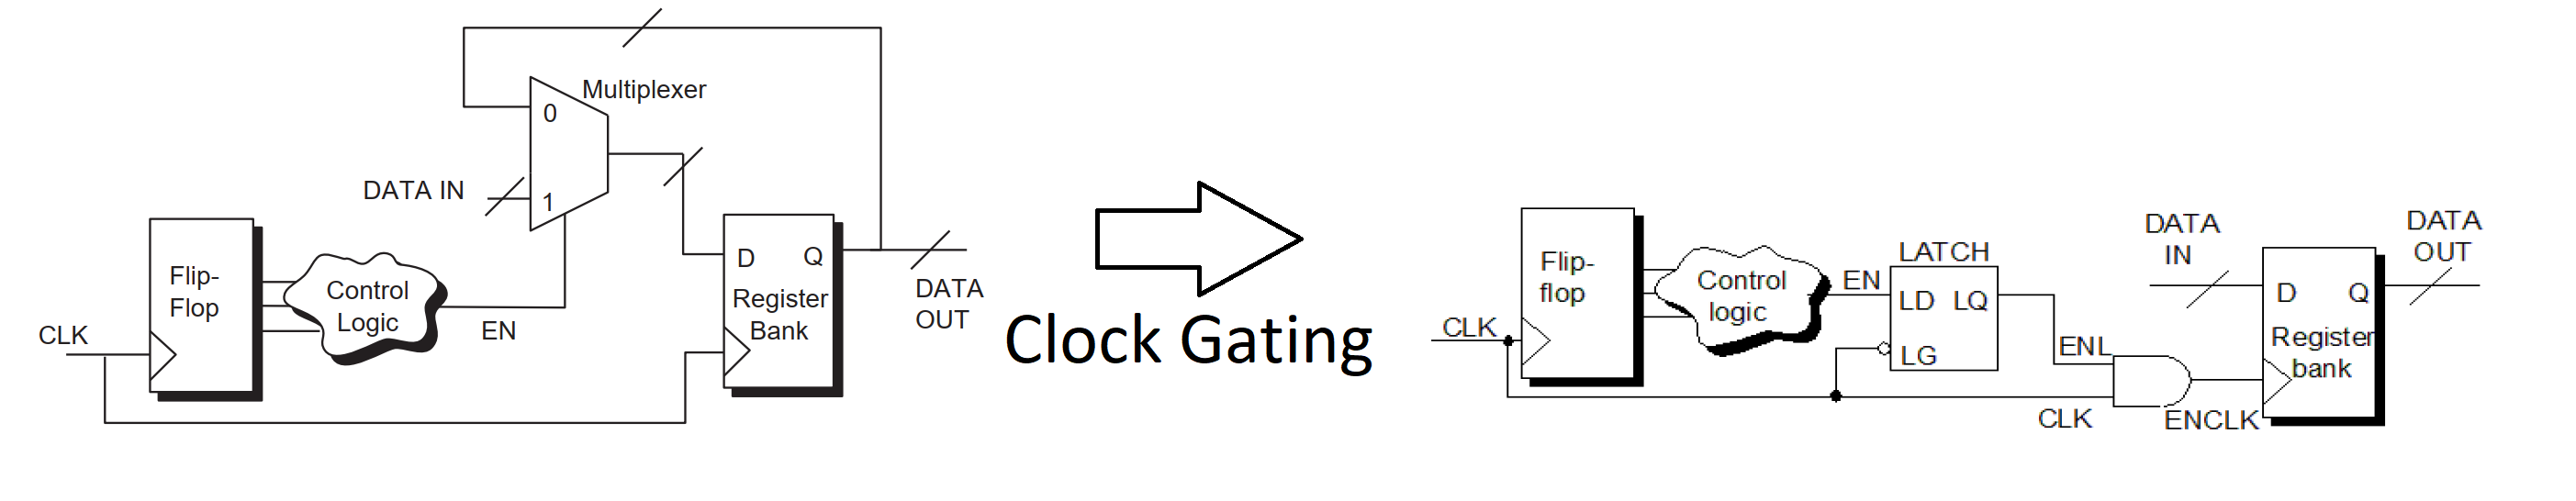
\includegraphics[width=1.0\textwidth]{./img/clock_gating}
  \caption{Optimización de potencia interna mediante la técnica de Clock Gating~\cite[Adaptado de][]{power_compiler_ug}.}
  \label{fig:clock_gating}
\end{figure}

Al final de la síntesis se obtiene el netlist de nivel compuertas el cual es procesado con IC Compiler 2 para realizar el PnR. A partir de los reportes de síntesis se obtienen los siguientes resultados: el área total de las celdas es \SI{55348}{\micro\meter\squared}, y la estimación de consumo de potencia es \SI{169.5}{\micro\watt}.

Después del script de síntesis se usa la herramienta Formality de Synopsys para verificar formalmente la equivalencia entre la lógica representada en el RTL y en el netlist de post síntesis. Este proceso es realizado mediante métodos formales y no requiere vectores de simulación~\cite[traducido de][]{formality_ug}. Design Compiler produce un archivo SVF que contiene información de orientación sobre los cambios realizados en el proceso de síntesis, por ejemplo: el renombramiento de registros, o el agregado de celdas de Clock Gating. En el proceso conocido como Matching, Formality usa este archivo para encontrar puntos de comparación comunes entre los dos diseños. Un punto de comparación puede ser una salida del diseño o un registro. Desde un punto de comparación Formality determina un cono lógico moviendo atrás que incluye toda la lógica que conecta a ese punto, hasta llegar a otro punto de comparación o una entrada del diseño. La \figref{fig:logic_cones} muestra un cono lógico. Después en el proceso de verificación Formality compara formalmente los conos de los dos diseños por cada punto de comparación.

\begin{figure}[htb]
  \centering
  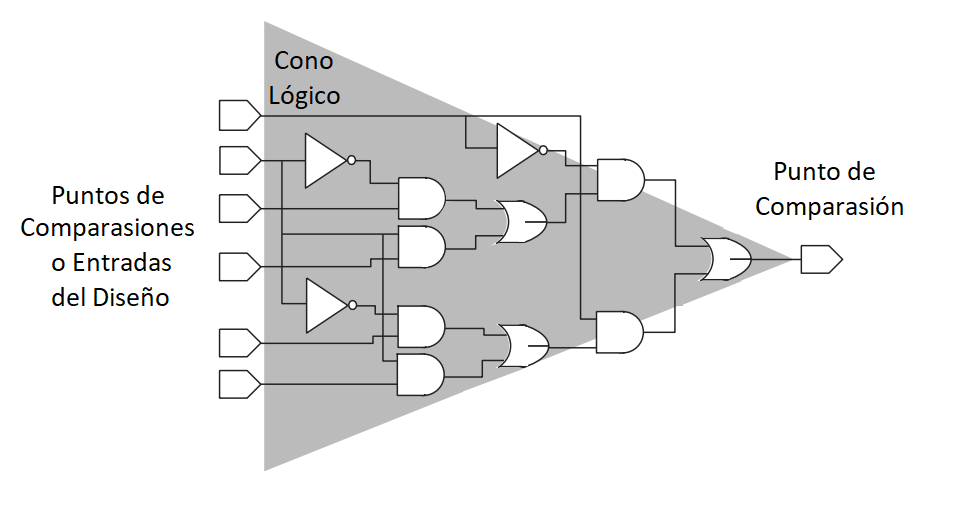
\includegraphics[width=1.0\textwidth]{./img/logic_cones}
  \caption{Un cono lógico~\cite[Adaptado de][]{formality_ug}.}
  \label{fig:logic_cones}
\end{figure}

% Preparación de librerías
% --------------------------------
\FloatBarrier
\section{Preparación de librerías}

IC Compiler 2 requiere las CLIBs (Cell Libraries) en el formato NDM (New Data Model). Al tiempo de realizar este trabajo XFAB no tenía disponible bibliotecas en el formato NDM por el proceso XH018. Por lo tanto es necesario convertir las bibliotecas provistas al formato NDM. Este proceso es realizado mediante la herramienta Library Manager de Synopsys. Cada celda en un NDM contiene información de timing, potencia, lógica, el layout físico y las reglas de la tecnología. En las CLIBs provistas por XFAB, esa información es contenido en bibliotecas de varios formatos:

\begin{itemize}
  \item TF: Las reglas de la tecnología.
  \item TLU: Información sobre parásitos.
  \item GDS: El layout de las celdas.
  \item LEF: Información sobre el layout de las pines y obstrucciones, e información sobre los propiedades antena de las celdas.
  \item DB: Información sobre timing, potencia y la lógica de las celdas.
\end{itemize}

Un script TCL fue diseñado para cargar todas esas bibliotecas y combinar la información a tres CLIBs en el formato NDM para uso con IC Compiler 2. Las tres CLIBs son:

\begin{itemize}
  \item tech\_only.ndm: Contiene información sobre la tecnología, esta incluye: las reglas de la tecnología, los parasíticos y las direcciones del ruteo en cada capa de metal (Horizontal o Vertical).
  \item d\_cells\_hd.ndm: Contiene información sobre las celdas estándares de D\_CELLS\_HD.
  \item d\_cells\_hdll.ndm: Contiene información sobre las celdas estándares de D\_CELLS\_\-HDLL.
\end{itemize}

El proceso para producir las CLIBs por las celdas estándares es: leer los archivos: TF, GDS, LEF y DB, y arreglar las discrepancias entre las descripciones de las celdas en cada formato. Por ejemplo: Los archivos GDS usan los nombres: vdd! y gnd! para los rails de alimentación, pero los archivos LEF usan los nombres: vdd y gnd.

% Design Planning
% --------------------------------
\FloatBarrier
\section{Design Planning}

Design Planning (DP) es un paso inicial de la implementación de un IC. En este trabajo el script de DP es principalmente usado para construir un floorplan (la forma y las dimensiones físicas del bloque), elegir ubicaciones por los pines que conectan a las otros bloques (el AFE, el Sensor MOSFET de radiación, y el ADC), y armar los anillos, mallas y rails de alimentación.

El floorplan posee las dimensiones físicas del diseño, en este caso del circuito digital. Luego los diferentes bloques del proyecto serán instanciados en un top cell el cual requerirá el ruteo manual entre los mismos, los pines de entrada/salida y los pads de prueba. El área del floorplan por el circuito digital debe ser al menos suficiente para contener las celdas, y los anillos de potencia, pero frecuentemente es necesario dejar más espacio en el núcleo para evitar congestión de ruteo. El área de las celdas es calculada desde el netlist producido en síntesis, para este proyecto esto es: \SI{55347}{\micro\meter\squared}. El núcleo del floorplan es el área que contiene las celdas, y la tasa de utilización del núcleo es la proporción del núcleo que contiene esas celdas. Usando un proceso iterativo se determinó que la tasa de utilización del núcleo máxima para que el diseño cumple con timing es 75\%. Así el núcleo debería tener un área de \SI{73796}{\micro\meter\squared}, lo que se corresponde con una región cuadrada de lado \SI{272}{\micro\meter}. La documentación del PDK especifica que los anillos de alimentación deben tener un ancho de \SI{5}{\micro\meter}, con separación de \SI{2.5}{\micro\meter}~\cite{dig_imp_guidelines}. Hay un anillo de VDD y uno de GND, así se necesita \SI{12.5}{\micro\meter} alrededor del núcleo. Esto significa que el floorplan tiene dimensiones de \SI{297}{\micro\meter} por \SI{297}{\micro\meter}, y un área total de \SI{88209}{\micro\meter\squared}. Debido a la forma de las celdas, la herramienta eligió las dimensiones: \SI{295.68}{\micro\meter} por \SI{294.0}{\micro\meter} dando un área de \SI{86930}{\micro\meter\squared}.

Este bloque está diseñado para ser conectado con los otros bloques del diseño internamente al IC, por eso es necesario agregar un pin por cada entrada y salida alrededor del núcleo. Esas pines son agregadas en las capas de metal: MET3 y MET4. Se ha considerado los siguientes criterios por los pines de interfaz con los bloques circuitales periféricos:

\begin{itemize}
  \item Señales desde / hacia el AFE están en el borde superior, en MET4.
  \item Señales hacia el Sensor están en la mitad inferior del borde derecho, en MET3.
  \item Señales desde / hacia el ADC están en la mitad superior del borde derecho, en MET3.
  \item Las entradas del UID están juntas pero no son constrained a un borde en particular. La herramienta eligió el borde izquierdo en MET3.
\end{itemize}

Las celdas estándares provistas en el PDK son diseñadas para tener la misma altura, con un rail de alimentación en el borde superior y un rail de tierra en el borde inferior, los dos en la primera capa de metal: MET1. La \figref{fig:xor_cell} muestra un ejemplo de una celda XOR con los rails de alimentación nombrados. Las celdas son fijadas en filas cruzando el núcleo del diseño, cada fila adicional se instancia de forma espejada para que compartan los rails. Es necesario conectar estos rails a los anillos y mallas de VDD y GND, mientras minimizando la caída de tensión debido a la resistencia parásita de las metalizaciones (caída IR). Los anillos rodean el núcleo, las mallas consisten en stripes (tiras) que cruzan el núcleo y los rails conectan las celdas con las mallas y anillos. La documentación del PDK~\cite{dig_imp_guidelines} específica que los anillos y mallas deben colocarse en las capas de metal superiores: METTP y METTPL, con ancho mínimo de 5 um, y separación máximo entre mallas de 350 um. METTP debe ser usado por las rutas horizontales y METTPL por las rutas verticales. Debido a que este bloque tiene dimensiones menores que 350 um por 350 um, las mallas de VDD y GND solo consisten en un stripe vertical y uno horizontal cruzando el centro del núcleo por las dos mallas. La \figref{fig:floorplan_pg} muestra el floorplan generado con las rutas de potencia y los pines de las entradas y salidas.

\begin{figure}[htb]
  \centering
  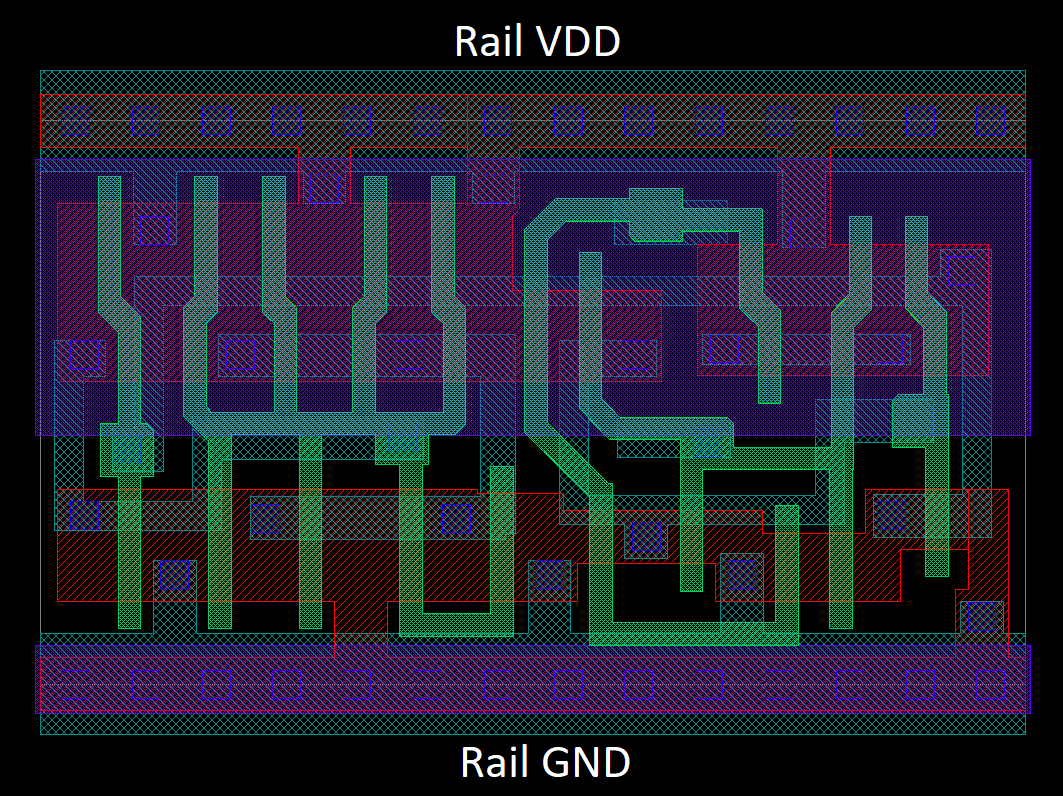
\includegraphics[width=0.8\textwidth]{./img/xor_cell}
  \caption{Una celda XOR de la biblioteca D\_CELLS\_HD.}
  \label{fig:xor_cell}
\end{figure}

Para poder conectar VDD y GND a la fuente de potencia en el AFE, es necesario agregar terminales. Debido a que los otros pines que conectan al AFE están en el borde superior, los terminales son colocados en el medio del borde superior de los anillos. La documentación del PDK~\cite{dig_imp_guidelines} específica que la caída de tensión máxima entre los anillos y los stripes debe ser menor que \SI{100}{\milli\volt}. Esto es verificado con las herramientas realizando un análisis de caída IR. Asumiendo un consumo de potencia máxima de \SI{400}{\micro\watt} lo que es casi doble la estimación de potencia final, los resultados de este análisis son: por VDD la caída IR máximo es \SI{34}{\micro\volt}, y por GND es \SI{38}{\micro\volt}. Estos resultados son aproximadamente 0,036\% de la máxima especificada en el PDK. La \figref{fig:ir_drop} muestra un mapa de calor del análisis de IR Drop para VDD.

\begin{figure}[htb]
  \centering
  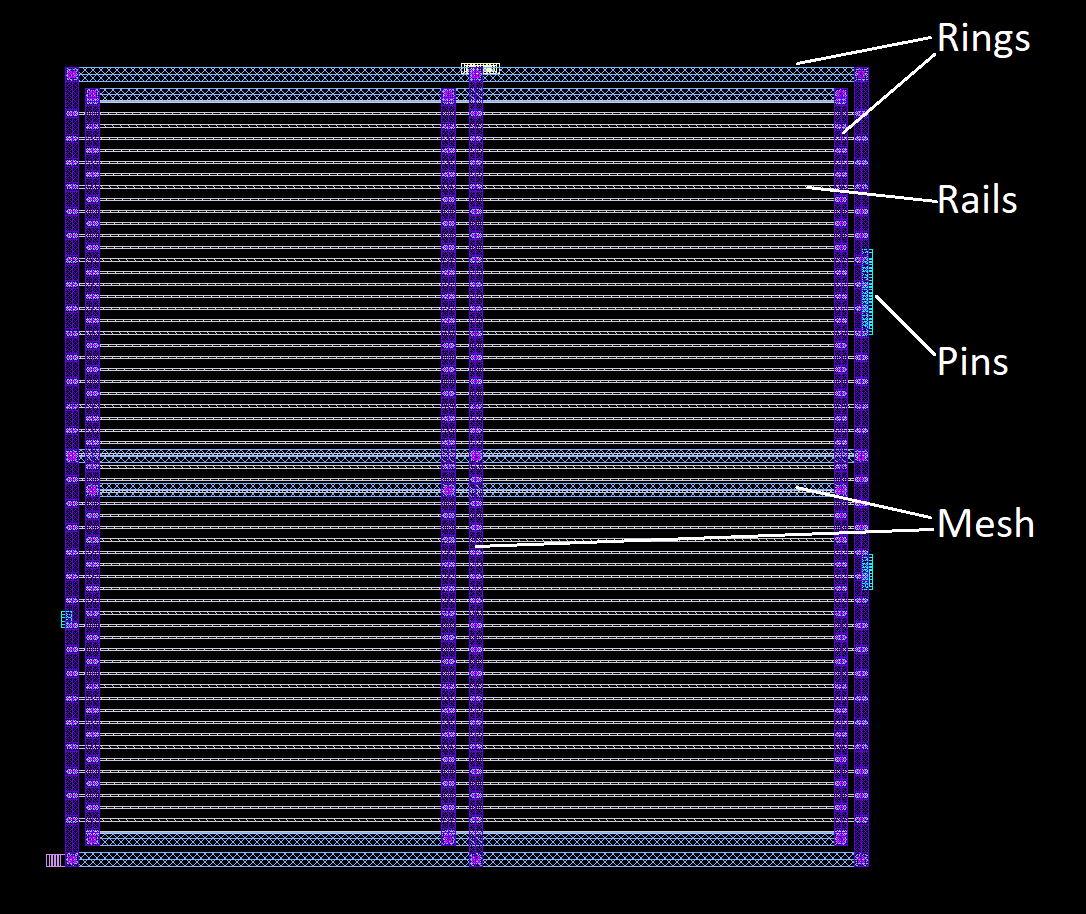
\includegraphics[width=0.9\textwidth]{./img/floorplan}
  \caption{El floorplan del diseño con las rutas de potencia y los pines IO.}
  \label{fig:floorplan_pg}
\end{figure}

\begin{figure}[htb]
  \centering
  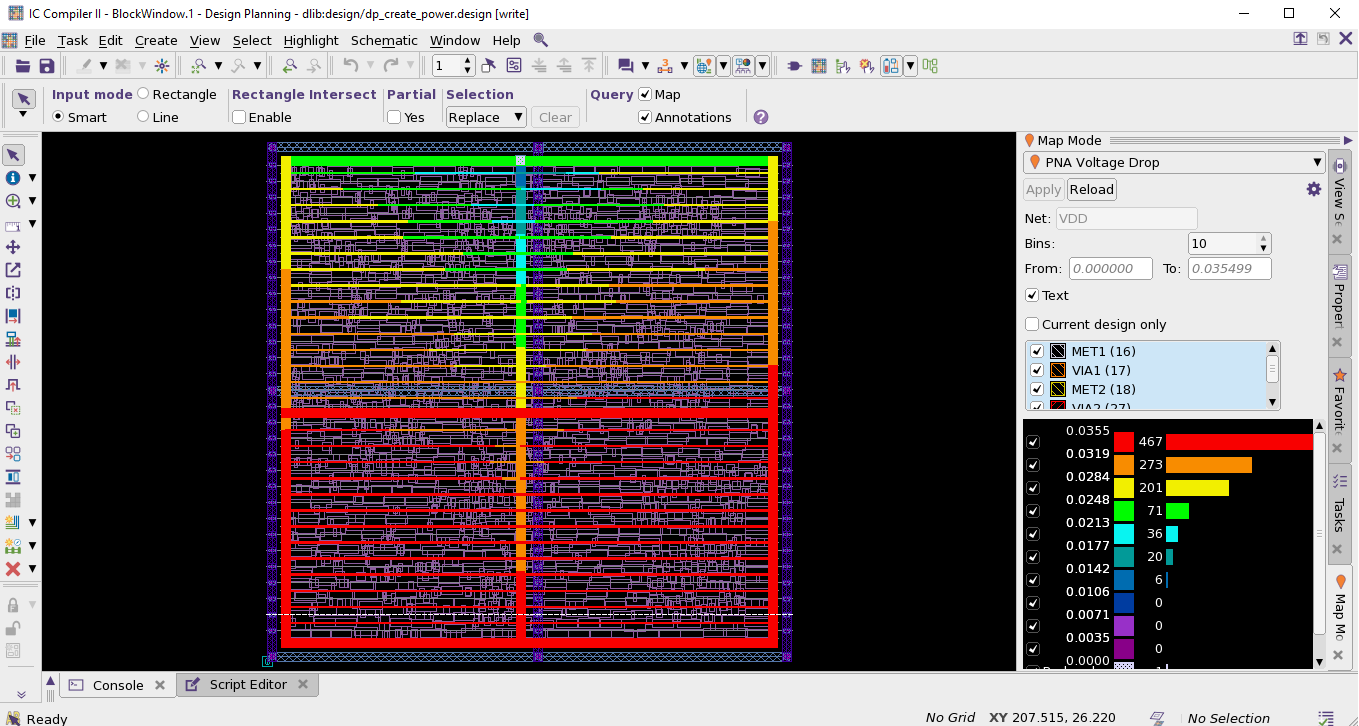
\includegraphics[width=0.9\textwidth]{./img/dp_create_power_ir_drop}
  \caption{Mapa de calor del análisis de caída IR sobre la ruta de alimentación VDD.}
  \label{fig:ir_drop}
\end{figure}


% Place & Route
% --------------------------------
\FloatBarrier
\section{Place \& Route}

El script de PnR comienza con la importación de los resultados de los script de Design Planning y de síntesis. Después las celdas son colocadas en el núcleo, este proceso es iterativo con múltiples de pasos para optimizar la ubicación de las celdas. Primero las celdas son colocadas de forma aproximada. Después las ubicaciones son ajustadas para optimizar por timing, área, consumo de potencia, y congestión. Después de cada paso los errores de DRC son arreglados.

La próxima operación es CTS (Clock Tree Synthesis), el proceso de construir y rutear árboles de relojes balanceados mediante buffers. Es necesario usar un árbol porqué el fanout del net del reloj es grande, ya que tiene que conectar a cada registro en el dominio del reloj. Tiene que ser balanceado para minimizar el skew en el reloj entre cada registro. Los reportes especifican que el skew máximo después de CTS es \SI{1.59}{\nano\second} en el análisis de Setup, y \SI{1.77}{\nano\second} en el análisis de Hold, los que son respectivamente 2,1\% y 2,4\% del periodo del reloj.

Durante el ruteo de los nets en el diseño es necesario tener cuidado sobre el largo de cada segmento de metal en la ruta, para evitar efectos de antenas. Synopsys define el problema de antenas como:

\begin{displaycquote}[traducido de][]{icc2_imp_ug}
  En la fabricación de circuitos integrados, el óxido de gate puede ser dañado fácilmente por descargas electrostáticas. La carga estática que es acumulada en las rutas de metal durante el proceso de metalización puede dañar el dispositivo o terminar con un fallo del chip entero.
\end{displaycquote}

El PDK contiene reglas de antenas que especifican los ratios máximos entre las áreas de los segmentos de metal y de los gates de los transistores de que se conectan~\cite{xh018_design_rules}. Si un diseño cumple con esas reglas, no debería tener problemas de antena. Una forma de arreglar estos problemas es cortar segmentos de metal grandes con un segmento en una capa de metal superior cercana al gate. Otra forma es colocar diodos cercanos a los gates. Cuándo las reglas de antena son agregadas, IC Compiler 2 intenta rutear el diseño evitando problemas de antenas, si siguen existiendo violaciones de antenas las celdas de diodos presentes en el PDK pueden ser agregadas.

La operación de ruteo también es un proceso iterativo, en el cual, en cada paso, se intenta arreglar las violaciones de DRC o de timing del paso anterior. Al final de este proceso el slack de Setup es \SI{2.6}{\nano\second}, y el slack de Hold es \SI{0.0}{\nano\second}. Los reportes indican que no hay violaciones DRC, ni problemas de antena, tampoco hay rutas abiertas o cortocircuitos.

Después del ruteo vienen dos acciones conocidas juntas como Finishing. La primera acción es agregar vías redundantes dónde hay espacio, para mejorar las conexiones entre las capas, esto se hace con un script del PDK. Después se agregan celdas de relleno (filler cells) en los espacios vacíos, esto es para asegurar que los rails de alimentación están conectados a lo largo de la fila. Hay dos tipos de celdas de relleno: con capacitores de desacople, y sin capacitores de desacople. Las celdas con capacitores son usadas para ayudar a mantener las rails de alimentación de forma local durante periodos de alto consumo de corriente. Esas celdas son agregadas primero, y las que generan errores DRC son quitadas. Después, los sitios que se quedan vacíos son llenados con las celdas sin capacitores. Finalmente el proceso de ruteo es ejecutado de nuevo en caso que haya que arreglar violaciones DRC. La \figref{fig:pnr_out} muestra el layout después del finishing.

\begin{figure}[htb]
  \centering
  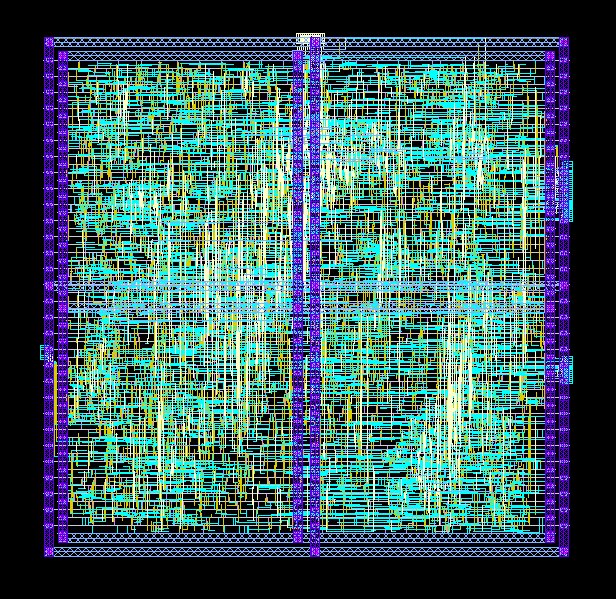
\includegraphics[width=0.8\textwidth]{./img/pnr_out}
  \caption{El layout del diseño después del finishing.}
  \label{fig:pnr_out}
\end{figure}

La próxima etapa es ICV In Design, esa etapa ejecuta unas acciones mediante la herramienta Synopsys IC Validator. La primera acción es verificar que no hay ninguna violación DRC en el diseño mediante un script provisto en el PDK, y si hay violaciones, intenta corregirlas. El próximo paso es el proceso de Metal Fill. Para reducir errores en el proceso de fabricación es necesario asegurar que la densidad de metal de cada capa está dentro de unos límites definidos en las reglas de diseño. Si la densidad de metal en una capa es demasiado baja, IC Validator puede agregar metal extra en los espacios libres. Después del metal fill, las pruebas DRC son ejecutadas de nuevo, pero esta vez activando una prueba opcional para verificar la densidad de metal.

El siguiente paso es escribir los resultados del PnR. El netlist final es exportado en dos formatos, uno para uso en LVS (Layout Vs Schematic) y uno para uso en el script de verificación de equivalencia con Formality. El layout final es guardado en el formato GDS~II.

La estimación de consumo de potencia final es \SI{256.0}{\micro\watt}, compuesta de: \SI{163.5}{\micro\watt} (64,0\%) potencia interna, \SI{91.6}{\micro\watt} (35,8\%) potencia dinámica, y \SI{623.8}{\nano\watt} (0,2\%) potencia estática. Análisis de timing indica que el mínimo Setup slack es \SI{1,59}{\nano\second} y el mínimo Hold slack es \SI{0.02}{\nano\second}. La \figref{fig:setup_hold_slack} muestra la distribución de slack de Setup y slack de Hold. Los dos rutas con menor Setup slack son 1) La ruta entre el registro de \textit{lm\_out} en el módulo \textbf{tx}, y la salida \textit{lm\_out} de este diseño. 2) La ruta entre la entrada \textit{pause\_n\_async} de este diseño y el primer registro en el módulo \textbf{pause\_n\_latch\_and\_synchroniser}. Estas rutas tienen slack bajo por los constraints: “set\_max\_delay 5.0”, los cuales están presentes para minimizar los retardos en la ruta del FDT.

\begin{figure}[htb]
  \centering
  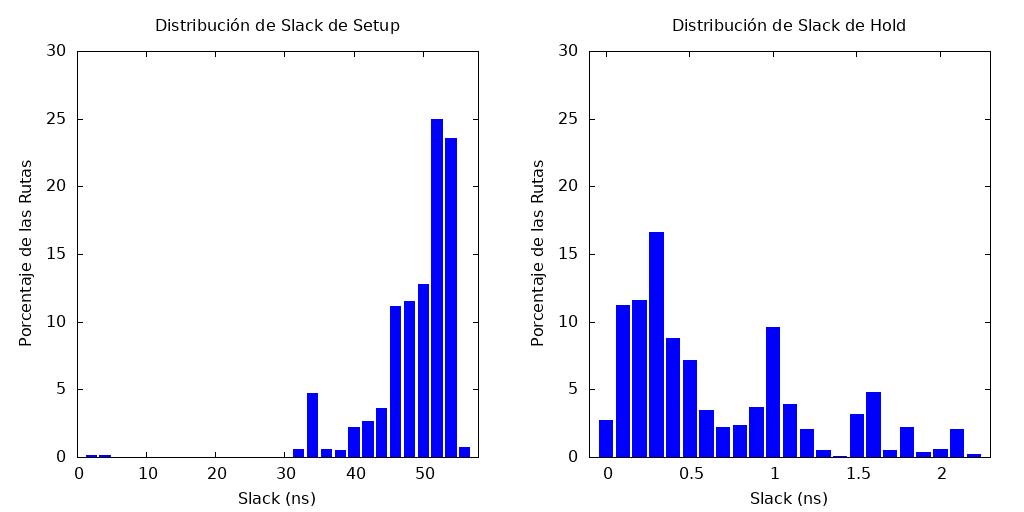
\includegraphics[width=0.8\textwidth]{./img/slack}
  \caption{Distribución de slack de Setup y de Hold en el diseño final.}
  \label{fig:setup_hold_slack}
\end{figure}

Finalmente la herramienta Formality es usada de nuevo para verificar formalmente la equivalencia de la lógica entre el RTL y el netlist de post implementación. Este proceso es equivalente del proceso hecho después de síntesis, salvo por que se usa los archivos SVF de coordinación generados en Design Planning y en Place \& Route, en adición a lo de síntesis.

% LVS / DRC
% --------------------------------
\FloatBarrier
\section{LVS / DRC}

En el script de Place \& Route el diseño fue analizado para verificar violaciones DRC, este paso es repetido en este punto pero usando el archivo GDS II e instanciando la herramienta IC Validator directamente. La ventaja de esto es que verifica que no haya errores DRC introducidos en el proceso de escribir el GDS II.

LVS (Layout Vs Schematic) es un análisis que compara la netlist final del diseño con el GDS II. La primera parte de esta operación es convertir el netlist de nivel compuertas escrito al final del script de PnR a un netlist de nivel SPICE mediante la herramienta nettran. Después IC Validator es ejecutado con un script provisto en el PDK para extraer los dispositivos y nets del layout en el archivo GDS II. Ese resultado es comparado con el netlist de nivel SPICE para confirmar que se corresponden.

% ---------------------------------------------
% Conclusión
% ---------------------------------------------

\FloatBarrier
\chapter{Conclusión}

En este trabajo un circuito digital fue implementado, verificado mediante simulaciones y preparado para fabricación con el proceso XFAB XH018. El circuito implementado permite la lectura de un sensor de forma inalámbrica mediante un protocolo propietario implementado encima del estándar ISO/IEC 14443A. En este caso el sensor es un dosímetro MOSFET de radiación ionizante para aplicación al control en tratamientos de radioterapia. Sin embargo el circuito digital diseñado no está limitado a esta aplicación y puede trabajar con diferentes sensores para otras aplicaciones sin necesidad de modificación alguna. Los bloques externos necesarios para este uso son: un AFE (Analogue Front End) conforme con ISO/IEC 14443-2A, un ADC de 16 bits, y el sensor propiamente dicho. La implementación del estándar ISO/IEC 14443A fue diseñado como un núcleo IP genérico, cuyo código RTL y los scripts de síntesis y PnR están disponibles en GitHUB de forma abierta bajo la licencia GNU v3.0. Esto significa que puede ser usado en otros proyectos académicos o comerciales, siempre que cumplan con las condiciones de la licencia.

En este proyecto, fue clave que el núcleo IP ISO/IEC 14443A sea genérico, para que funcione con AFEs distintas. Para ello las propiedades más importantes son el comportamiento del reloj y la pausa detectada. Por lo tanto:

\begin{itemize}
  \item El núcleo IP incluye un módulo asincrónico para la retención de pausas en el caso que el AFE no pueda garantizar que haya un flanco ascendente del reloj durante las pausas.
  \item El módulo \textbf{sequence\_decode} fue diseñado para decodificar las tramas correctamente aún cuando el reloj está detenido, hasta un máximo de 59 ciclos, durante las pausas, incluyendo el caso de un reloj continuo.
  \item El núcleo IP lleva un parámetro \textit{FDT\_TIMING\_ADJUST} que permite el ajuste del temporizador en el módulo \textbf{FDT} para compensar por los retrasos externos en la ruta del FDT.
\end{itemize}

Uno de los objetivos de esta tesis fue la posibilidad de tomar muestras de múltiples de PICCs de forma sincronizada. Para cumplir con este objetivo se propone una solución mediante el protocolo a nivel de aplicación. Este protocolo utiliza dos características del sistema: 1) Todas las PICCs extraen el reloj de la misma portadora y por lo tanto sus relojes son sincrónicos, 2) todas las PICC reciben las pausas en el mismo instante. Además se implementa una lectura del ADC y del sensor de manera automatizada y parametrizable. Aprovechando estas características es posible realizar la lectura sincrónica de todos los sensores que estén en el rango del PCD.

Todo el RTL implementado es verificado con una serie de bancos de pruebas exhaustivas, con 60 horas de simulaciones. Los bancos de pruebas contienen 187 aserciones que son ejecutados casi cien millones de veces en total, sin fallar siquiera una vez. Cada simulación genera un informe de cobertura y en todos los casos se observan resultados favorables. Además el modelo del AFE implementado permite la configuración de varias de sus propiedades para simular el comportamiento de diferentes AFEs. Finalmente el RTL se verifica formalmente, mediante una cadena de equivalencias: el RTL es equivalente al netlist post implementación, y a su vez este netlist es equivalente al layout del diseño.

Los reportes finales indican que:

\begin{itemize}
  \item El diseño contiene 595 registros (568 de esos son gated), 2017 compuertas combinacionales y 2706 nets.
  \item El consumo de potencia promedio estimado es \SI{256}{\micro\watt}, compuesto de: \SI{163}{\micro\watt} potencia interna, \SI{92}{\micro\watt} potencia dinámica, y \SI{624}{\nano\watt} potencia estática. Esta estimación está basada en una simulación de la inicialización de la PICC y cinco muestras del sensor.
  \item El área total del diseño es \SI{86930}{\micro\meter\squared} = \SI{0.087}{\milli\meter\squared} (\SI{295.68}{\micro\meter}, \SI{294.00}{\micro\meter}).
  \item No hay slack negativo de Setup. El menor slack de Setup es \SI{1.59}{\nano\second} y ocurre en la ruta entre el registro de \textit{lm\_out} en el módulo \textbf{tx}, y la salida \textit{lm\_out} del diseño entero. Esa ruta tiene un slack bajo por el constraint: “set\_max\_delay 5.0 -to [get\_ports lm\_out]”, el cual está presente para minimizar los retardos en la ruta del FDT. El mínimo slack de setup que corresponde a una ruta sin un constraint de set\_max\_delay tiene un valor de \SI{32.26}{\nano\second}.
  \item No hay slack negativo de hold. El slack mínimo es \SI{0.02}{\nano\second}.
  \item El diseño pasa sin errores las verificaciones de DRC y LVS.
  \item La lógica en el netlist post-implementación es equivalente a la del RTL.
\end{itemize}

Todos estos resultados dan una excelente confianza en el diseño. Debido a las suposiciones asumidas sobre otros bloques aún no diseñados, es altamente recomendable revisar el correcto funcionamiento del sistema completo antes de su fabricación, para verificar la correcta interoperabilidad entre todos los bloques.

% Requisitos para los otros bloques
% --------------------------------
\FloatBarrier
\section{Requisitos para los otros bloques}

Para asegurar el funcionamiento correcto de un ASIC que incluya el diseño elaborado en esta tesis, los otros bloques presentes deben cumplir con algunos requisitos. El sensor y el ADC deben operar de forma que se puede tomar una muestra mediante la operación mostrado en la \figref{fig:sens_adc}. Los valores de $t_1$ y $t_2$ requeridos para tomar una muestra correcta deben ser menor que $\SI{33554431}{ciclos} \approx \SI{2.47}{\second}$. El AFE debe cumplir con los siguientes requisitos:

\begin{itemize}
  \item Debe ser conforme con la norma ISO/IEC 14443-2A.
  \item Debe recuperar el reloj desde la portadora transmitida por el PCD. El reloj recuperado debe ser monótono y no tener glitches. Si se detiene durante las pausas debe hacerlo por un tiempo menor a 59~ciclos, aunque se recomienda que el tiempo sea menor a 56~ciclos, de esta manera el sistema tolera hasta $\pm 3$~ciclos de jitter en la detección de la pausa.
  \item Para minimizar el retardo en la ruta del FDT, el reloj debe comenzar de nuevo lo antes posible y el fin de la pausa también debe ser detectado lo antes posible. Además debe minimizarse el retardo de propagación entre la salida \textit{lm\_out} de este diseño y el modulador de carga.
  \item Cuándo la PICC entra en un campo electromagnético, la señal de reset \textit{rst\_n\_async} debe estar ‘0’ hasta que el rail de alimentación VDD y la entrada \textit{uid\_variable} de este diseño están estables.
  \item La salida \textit{afe\_version[3:0]} debe ser constante.
  \item La salida \textit{power[1:0]} debe ser estable durante 512 ciclos después de una pausa. Esto es para prevenir metastabilidad en el muestreo de esta señal.
\end{itemize}

El diseñador del AFE debe considerar las restricciones impuestas en la forma de la pausa especificadas en la norma ISO/IEC 14443-2A, y asegurarse que su diseño cumple con esos requisitos por cualquiera forma de la pausa válida.

% Recomendaciones para Trabajos Futuros
% --------------------------------
\FloatBarrier
\section{Recomendaciones para Trabajos Futuros}

A continuación se listan trabajos que quedan fuera del alcance de esta tesis pero serían necesarios para la fabricación del chip considerado en el proyecto marco:

\begin{itemize}
  \item Realizar una mejor estimación del consumo de potencia, incluyendo consumo pico. Esto es importante al momento de diseñar el AFE.
  \item Realizar simulaciones de nivel compuerta para verificar el diseño post síntesis y post PnR.
  \item Implementar el AFE, el ADC y el sensor en la tecnología XH018 de X-Fab.
  \item Agregar puntos de prueba al diseño para permitir realizar mediciones e inyectar señales de forma directa.
  \item Fabricar y medir el IC.
\end{itemize}

Además existen algunas características extras que podrían ser implementadas en el núcleo IP ISO/IEC 14443 para que sea adecuado para uso en un rango más amplio de proyectos:

\begin{itemize}
  \item Agregar soporte para tags de tipo B.
  \item Implementar las partes opcionales de la norma: soporte para las otras tasas de bits, NADs, bloques estándares encadenados, los bloques estándares S(PARAMETERS) y S(WTX), y bloques aumentados~\cite{iso14443-2}\cite{iso14443-4}.
\end{itemize}

% ---------------------------------------------
% Appendices
% ---------------------------------------------

\appendix

% Change the \chapter rules to use numbersr for the appendices
\titleformat{\chapter}[display]
{\normalfont\Huge\bfseries}{\chaptertitlename\ \thechapter:}{0.2em}{\huge}

% Repositorio de código fuente
% ----------------------------
\newpage
\chapter{Repositorio de Código Fuente}
\label{appendix:code_repo}

Todo el código RTL y los scripts usados en este trabajo están disponibles en un repositorio de GitHUB: \url{https://github.com/andrewparlane/fiuba_thesis}. El código y los scripts están disponible de forma abierta bajo la licencia GNU v3.0. Se puede clonar este repositorio con los comandos:

\begin{lstlisting}[language=bash,basicstyle=\small\ttfamily]
  git clone https://github.com/andrewparlane/fiuba_thesis.git
  git submodule update --init --recursive
\end{lstlisting}

La estructura del repositorio es:

\vspace{1em}

\dirtree{%
.1 fiuba\_thesis.
.2 hdl.
.3 components.
.4 iso\_iec\_14443A\DTcomment{Git Submodule del núcleo IP ISO/IEC 14443A}.
.3 rtl\DTcomment{RTL de la aplicación}.
.3 synth\_pnr\DTcomment{Scripts de síntesis y PnR}.
.3 verification.
.4 bfms\DTcomment{Clases y paquetes de verificación de la aplicación}.
.4 tb\DTcomment{Los bancos de pruebas de los módulos de la aplicación}.
.4 vcs\DTcomment{Contiene un Makefile para ejecutar las simulaciones}.
.5 reports\DTcomment{Logs e informes de cobertura de las simulaciones}.
.2 thesis\DTcomment{Fuente de este documento}.
}

La carpeta \textit{fiuba\_thesis/hdl/components} contiene un Git Submodule del repositorio del núcleo IP ISO/IEC 14443A: \url{https://github.com/andrewparlane/iso_iec_14443A}. También el código y los scripts están disponible de forma abierta bajo la licencia GNU v3.0. La estructura de este repositorio es:

\vspace{1em}

\dirtree{%
.1 iso\_iec\_14443A.
.2 rtl\DTcomment{RTL del núcleo IP}.
.2 verification.
.3 bfms\DTcomment{Clases y paquetes de verificación del núcleo IP}.
.3 tb\DTcomment{Los bancos de pruebas de los módulos del núcleo IP}.
.3 vcs\DTcomment{Contiene un Makefile para ejecutar las simulaciones}.
.4 reports\DTcomment{Logs e informes de cobertura de las simulaciones}.
}

% Definiciones del protocolo propietario
% ----------------------------
\newpage
\chapter{Definiciones del protocolo propietario}
\label{appendix:protocol_defs}

Este apéndice contiene un header del lenguaje de programación C con definiciones y estructuras del protocolo propietario de la aplicación.

% texcl=true means that comments (//) are treated as LaTeX. So we need a backslash before underscores or ampersands
\begin{lstlisting}[language=C, style=CStyle, texcl=true]
// La mágica y la versión del protocolo
#define PROTOCOL_MAGIC              0xF100BA00
#define PROTOCOL_VERSION            1

// Las mascaras de bits de las salidas al sensor / ADC
#define SIGNALS_MASK_SENS_CONFIG    0xE0
#define SIGNALS_MASK_SENS_ENABLE    0x10
#define SIGNALS_MASK_SENS_READ      0x08
#define SIGNALS_MASK_ADC_ENABLE     0x04
#define SIGNALS_MASK_ADC_READ       0x02

// Las mascaras de bits de los flags de estado
#define FLAGS_MASK_CONV_COMPLETE    0x80
#define FLAGS_MASK_ALREADY_BUSY     0x40
#define FLAGS_MASK_UNEXPECTED_PAUSE 0x20
#define FLAGS_MASK_ERROR            0x10

// Los mensajes definidos
enum Command
{
    Command_IDENTIFY    = 0,
    Command_SET_SIGNAL  = 1,
    Command_AUTO_READ   = 2,
    Command_GET_RESULT  = 3,
    Command_ABORT       = 4
};

// La cabecera
struct __attribute__((packed)) Header
{
    uint32_t    magic;  // PROTOCOL\_MAGIC
    uint8_t     cmd;    // enum Command, respuestas deben usar el mismo que el solicitud
};
// =============================================
// Solicitudes
// =============================================

// Comand\_IDENTIFY
struct __attribute__((packed)) IdentifyRequest
{
    struct Header   hdr;    // La cabecera
};

// Command\_SET\_SIGNAL
// Cambia las salidas al sensor / ADC:
//  nuevos = (anteriores \& $\sim$mask) $\vert$ (value \& mask);
// dónde nuevos, anteriores, mask, y value son mascaras de bits (SIGNALS\_MASK\_...)
struct __attribute__((packed)) SetSignalRequest
{
    struct Header   hdr;    // La cabecera
    uint16_t        sync;   // Tiempo de sincronización (t\_sync)
    uint8_t         mask;   // Mascara de bits
    uint8_t         value;  // Señales a cambiar
};

// Command\_AUTO\_READ
struct __attribute__((packed)) AutoReadRequest
{
    struct Header   hdr;        // La cabecera
    uint16_t        sync;       // Tiempo de sincronización (t\_sync)
    uint32_t        timing1;    // [24:0] Tiempo entre sens\_en/adc\_en y sens\_read
    uint32_t        timing2;    // [24:0] Tiempo entre sens\_read y adc\_read
};

// Comand\_GET\_RESULT
struct __attribute__((packed)) GetResultRequest
{
    struct Header   hdr;    // La cabecera
};

// Comand\_ABORT
struct __attribute__((packed)) AbortRequest
{
    struct Header   hdr;    // La cabecera
};


// =============================================
// Respuestas
// =============================================

// Command\_IDENTIFY
struct __attribute__((packed)) IdentifyReply
{
    struct Header   hdr;                    // La cabecera
    uint8_t         protocol_version;       // La versión de este protocolo
                                            // (PROTOCOL\_VERSION)
    uint8_t         adapter_version;        // La versión del adaptador (adapter.sv)
    uint8_t         iso_iec_14443a_version; // [7:4] versión del núcleo IP digital
                                            // [3:0] versión del AFE
    uint8_t         sensor_adc_version;     // [7:4] versión del sensor
                                            // [3:0] versión del ADC
};

// Command\_GET\_RESULT
struct __attribute__((packed)) GetResultReply
{
    struct Header   hdr;        // La cabecera
    uint8_t         flags;      // Flags de estado (FLAGS\_MASK\_...)
    uint16_t        adc_value;  // El último dato muestreado
};

// Respuesta a cualquier otro comando incluyendo los comandos inválidos.
struct __attribute__((packed)) StatusReply
{
    struct Header   hdr;    // La cabecera
    uint8_t         flags;  // Flags de estado (FLAGS\_MASK\_...)
};
\end{lstlisting}


% ---------------------------------------------
% Bibliography
% ---------------------------------------------

\FloatBarrier
\newpage

% Prevent overful hbox warning due to long titles
\emergencystretch=1em
\printbibliography
\emergencystretch=0em

\end{document}
